\documentclass[notheorems,compress,mathserif,table]{beamer}

\useoutertheme{tree}
\usecolortheme{whale}      % Outer color themes, 其他选择: whale, seahorse, dolphin . 换一个编译看看有什么不同.
\usecolortheme{orchid}     % Inner color themes, 其他选择: lily, orchid
\useinnertheme[shadow]{rounded} % 对 box 的设置: 圆角、有阴影.
\setbeamercolor{sidebar}{bg=blue!50} % sidebar的颜色, 50%的蓝色.
%\setbeamercolor{background canvas}{bg=blue!9} % 背景色, 9%的蓝色. 去掉下一行, 试一试这个.
\setbeamertemplate{background canvas}[vertical shading][bottom=white,top=structure.fg!25] %%背景色, 上25%的蓝, 过渡到下白.
\usefonttheme{serif}  % 字体. 个人偏好有轮廓的字体. 去掉这个设置编译, 就看到不同了.
\setbeamertemplate{navigation symbols}{}   %% 去掉页面下方默认的导航条.
%%------------------------常用宏包---------------------------------------------------------------------
%%注意, beamer 会默认使用下列宏包: amsthm, graphicx, hyperref, color, xcolor, 等等
%\usepackage{CJK}
\usepackage{ctex}
\usepackage{amsmath,amsthm,amsfonts,amssymb,bm}
\usepackage{mathrsfs}
\usepackage{subfigure} %%图形或表格并排排列
\usepackage{xmpmulti}  %%支持文中的 \multiinclude 等命令, 使 mp 文件逐帧出现. 具体讨论见 beamer 手册.
\usepackage{colortbl,dcolumn}     %% 彩色表格
%\logo{
\includegraphics[height=0.09\textwidth]{ajln.jpg}}   %左上角科大logo
%%%%%%%%%%%%%%%%%%%%%%%%%%%%%%%%%%%%%%重定义字体、字号命令 %%%%%%%%%%%%%%%%%%%%%%%%%%%%%%%%%%%%%%%%%%%%%%
%\newcommand{\songti}{\CJKfamily{song}}        % 宋体
%\newcommand{\fangsong}{\CJKfamily{fs}}        % 仿宋体
%\newcommand{\kaishu}{\CJKfamily{kai}}         % 楷体
%\newcommand{\heiti}{\CJKfamily{hei}}          % 黑体
%\newcommand{\lishu}{\CJKfamily{li}}           % 隶书
\newcommand{\youyuang}{\CJKfamily{you}}       % 幼圆
\newcommand{\sanhao}{\fontsize{16pt}{\baselineskip}\selectfont}     % 字号设置
\newcommand{\sihao}{\fontsize{14pt}{\baselineskip}\selectfont}      % 字号设置
\newcommand{\xiaosihao}{\fontsize{12pt}{\baselineskip}\selectfont}  % 字号设置
\newcommand{\wuhao}{\fontsize{10.5pt}{\baselineskip}\selectfont}    % 字号设置
\newcommand{\xiaowuhao}{\fontsize{9pt}{\baselineskip}\selectfont}   % 字号设置
\newcommand{\liuhao}{\fontsize{7.875pt}{\baselineskip}\selectfont}  % 字号设置
\newcommand{\qihao}{\fontsize{5.25pt}{\baselineskip}\selectfont}    % 字号设置
%%%%%%%%%%%%%%%%%%%%%%%%%%%%%%%%%%%%%%%%%%%%%%%%%%%%%%%%%%%%%%%%%%%%%%%%%%%%%%%%%%%%%%%%%%%%%%%%%%%%%%%%
%%----------------------- Theorems ---------------------------------------------------------------------
\newtheorem{theorem}{定理}
\newtheorem{definition}{定义}
\newtheorem{lemma}{引理}
\newtheorem{example}{例题}
\newtheorem{answer}{解:}
\newtheorem{dablock}{}
\newtheorem{jytg}{提纲}
\newtheorem{daproof}{证明}
\newtheorem{explain}{说明}
\newtheorem{summary}{小结}

\newtheorem{zhuyi}{注意}
\newtheorem{zhu}{注:}
\newtheorem{gongshi}{公式}
\newtheorem{shuoming}{说明}
\newtheorem{wenti}{问题}
\newtheorem{jielun}{结论}
\newtheorem{yinli}{引理}
%%----------------------------------------------------------------------------------------------------
\title{\heiti 第6章\quad  IIR数字滤波器的设计}
\author[\textcolor{blue}]{{\sihao\kaishu  笪邦友}}
\institute{\sihao\lishu  \textcolor{violet}{中南民族大学~~ 电子信息工程学院}}
\date{\fangsong\today} 

\begin{document}
	%  \begin{CJK*}{GBK}{kai}
	\kaishu
	\frame{ \titlepage }
	%%---------------------------------------------------------------------------------------------------
	\section*{目录}
	\frame[shrink]{\kaishu\frametitle{\kaishu 目录}\tableofcontents}
	
%\section{ 引言}
\section{6.1 滤波器概述}
%任意两行单列线表示一张ppt
%%---------------------------------------------------------------------------------------------------

%%%%%%%%%%%%%%%%%%%%%%%%%%%%%%%%%%%%%%%%%%%%%%%%%%%%%%%%%%%%%%%%%%%%%%%%%%%%%%%%%%%%%%%%%%%%%%
\subsection{6.1.1 滤波器的概念}
%%%%%%%%%%%%%%%%%%%%%%%%%%%%%%%%%%%%%%%%%%%%%%%%%%%%%%%%%%%%%%%%%%%%%%%%%%%%%%%%%%%%%%%%%%%%%%
\begin{frame}\frametitle{}%[allowframebreaks]6.1 滤波器概述
\textbf{\heiti 一、滤波器的概念}
\newline
滤波器是一种对信号频率具有选择性的系统。
\begin{figure}[h]
  \centering
  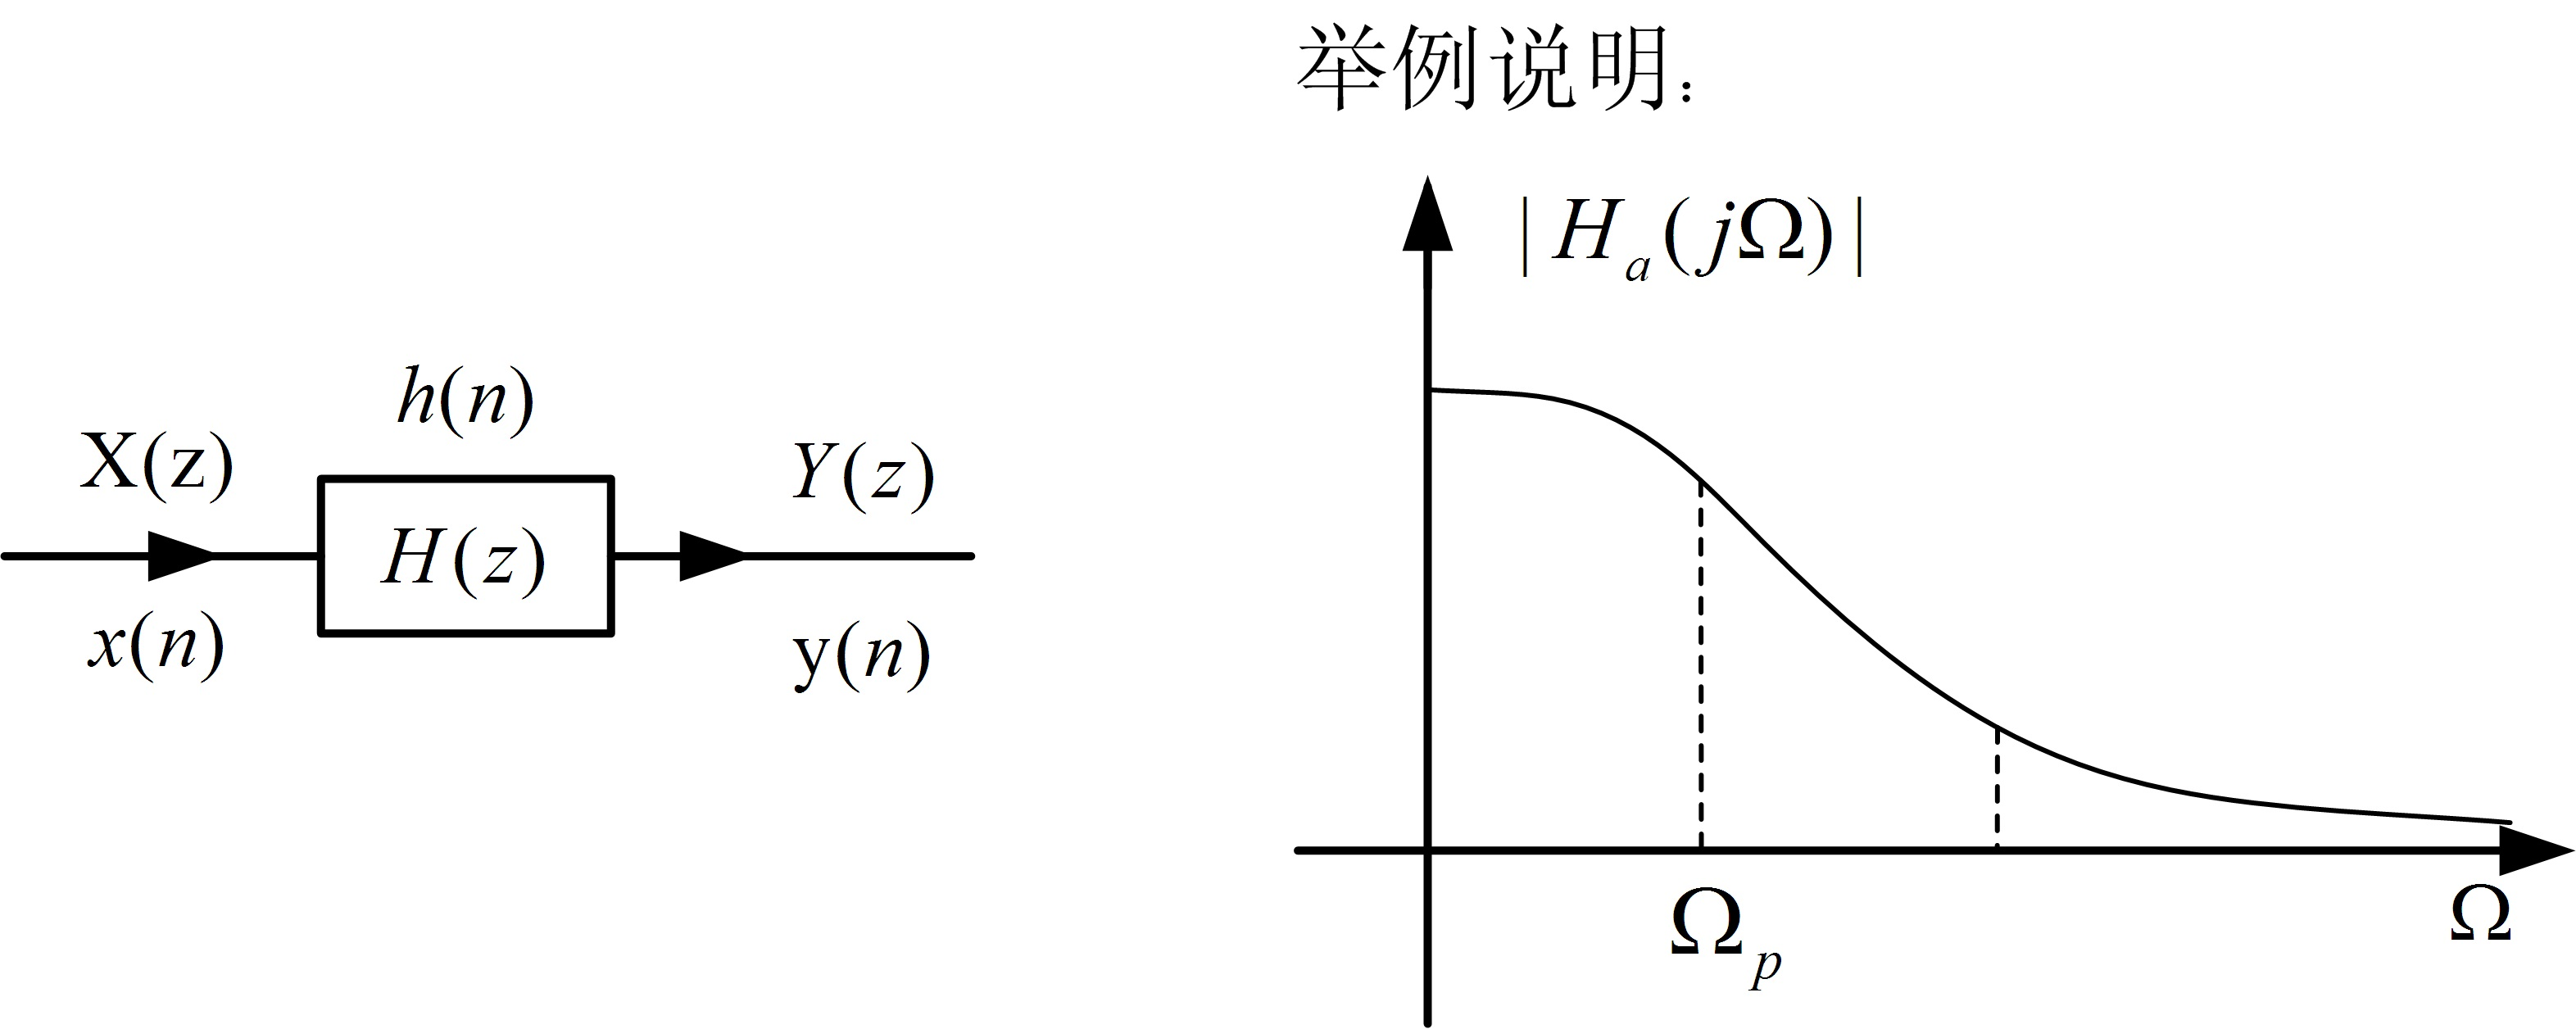
\includegraphics[width=0.9\textwidth]{fig1_lvboqigainian.jpg}
\end{figure}
\end{frame}

%%%%%%%%%%%%%%%%%%%%%%%%%%%%%%%%%%%%%%%%%%%%%%%%%%%%%%%%%%%%%%%%%%%%%%%%%%%%%%%%%%%%%%%%%%%%%%
%%%%%%%%%%%%%%%%%%%%%%%%%%%%%%%%%%%%%%%%%%%%%%%%%%%%%%%%%%%%%%%%%%%%%%%%%%%%%%%%%%%%%%%%%%%%%%
%\begin{frame}\frametitle{一、滤波器的概念}%[allowframebreaks]
%
%对线性时不变系统
%\end{frame}

%%%%%%%%%%%%%%%%%%%%%%%%%%%%%%%%%%%%%%%%%%%%%%%%%%%%%%%%%%%%%%%%%%%%%%%%%%%%%%%%%%%%%%%%%%%%%%

\subsection{6.1.2 理想滤波器与实际滤波器}
%%%%%%%%%%%%%%%%%%%%%%%%%%%%%%%%%%%%%%%%%%%%%%%%%%%%%%%%%%%%%%%%%%%%%%%%%%%%%%%%%%%%%%%%%%%%%%
\begin{frame}\frametitle{}%[allowframebreaks]
\textbf{\heiti 二、理想滤波器与实际滤波器}
$$\mbox{设}\quad\quad\quad\quad  H_{a}(j\Omega)=|H_{a}(j\Omega)|\cdot e^{jarg[H_{a}(j\Omega)]}$$

 (1) 理想滤波器
   $$|H_{a}(j\Omega)| = \left\{\begin{array}
         {r@{,\quad}l}
         1 &\mbox{$\Omega < \Omega_{p}$}\\
         0 &\mbox{$\Omega > \Omega_{p}$}
        \end{array} \right.
   $$

   \begin{figure}[h]
       \centering
       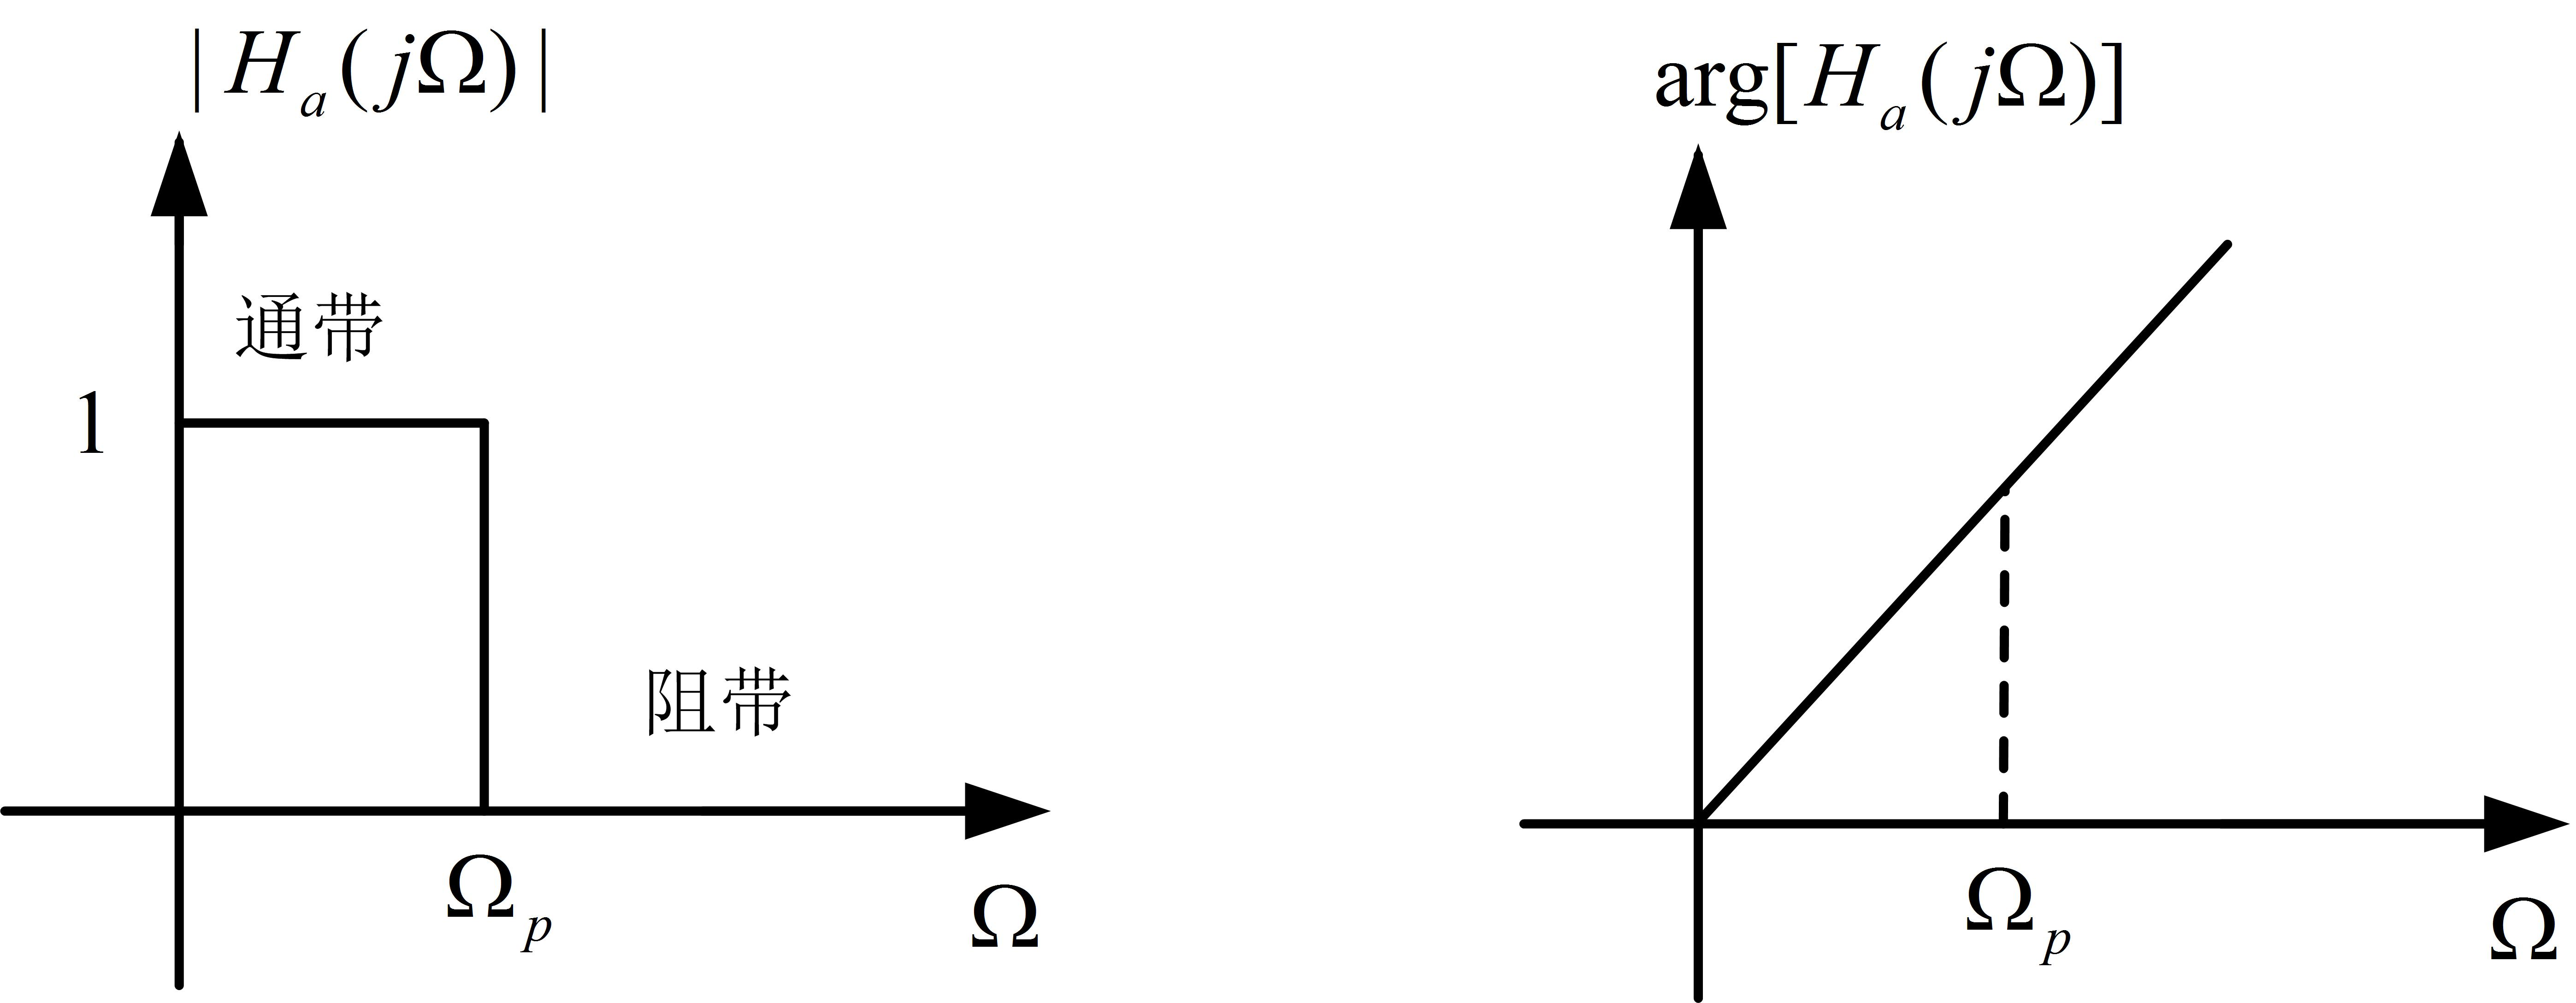
\includegraphics[width=0.7\textwidth]{fig2lxlbqtx.jpg}
       %\caption{理想滤波器的幅频特性与相频特性}
      %\label{}
   \end{figure}
  理想滤波器不可能用电子部件实现,因为其单位脉冲响应是非因果,且无限长。虽然其
   可在计算机上实现,但存在严重问题。

\end{frame}
%%%%%%%%%%%%%%%%%%%%%%%%%%%%%%%%%%%%%%%%%%%%%%%%%%%%%%%%%%%%%%%%%%%%%%%%%%%%%%%%%%%%%%%%%%%%%%
%%%%%%%%%%%%%%%%%%%%%%%%%%%%%%%%%%%%%%%%%%%%%%%%%%%%%%%%%%%%%%%%%%%%%%%%%%%%%%%%%%%%%%%%%%%%%%
\begin{frame}[shrink]\frametitle{}%[allowframebreaks]
(2)实际滤波器的形状
   \begin{enumerate}
     \item [1]实际滤波器不可能有理想的形状。
       \begin{figure}[h]
            \centering
            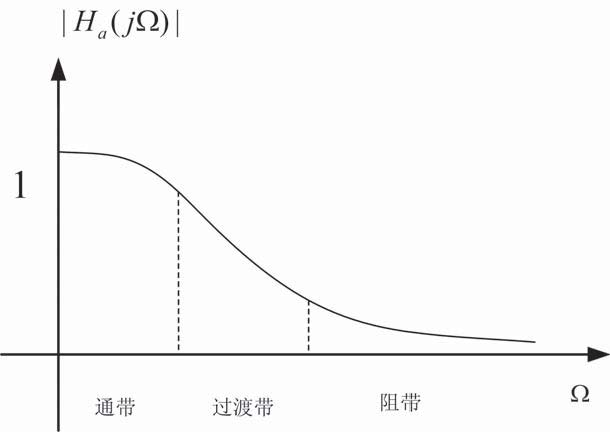
\includegraphics[width=0.7\textwidth]{fig3sjlbqtx.jpg}
            \caption{实际滤波器的幅频特性可能的形状}
        \end{figure}
     \item [2]三个概念
           \begin{enumerate}
             \item [(1)] 通带:滤波器中能使信号通过的频带;
             \item [(2)] 阻带:滤波器中不能使信号通过的频带;
             \item [(3)] 过渡带: 介于通带和阻带之间的频带。
           \end{enumerate}
  \end{enumerate}
\end{frame}

\subsection{6.1.3 滤波器的分类}
%%%%%%%%%%%%%%%%%%%%%%%%%%%%%%%%%%%%%%%%%%%%%%%%%%%%%%%%%%%%%%%%%%%%%%%%%%%%%%%%%%%%%%%%%%%%%%
\begin{frame}[shrink]\frametitle{}%[allowframebreaks]
\textbf{\heiti 三、滤波器的分类}

\begin{enumerate}
  \item[1]
     按处理信号的特性分:
      \begin{enumerate}
        \item [(1)] AF—模拟滤波器
        \item [(2)] DF—数字滤波器
      \end{enumerate}
      \par\quad%\newline
  \item[2]
       按通频带的的特性分:(选频数字滤波器)
      \begin{enumerate}
        \item [(1)] LP—低通滤波器
        \item [(2)] HP—高通滤波器
        \item [(3)] BP—带通滤波器
        \item [(4)] BS—带阻滤波器
      \end{enumerate}
\end{enumerate}
\end{frame}
%%%%%%%%%%%%%%%%%%%%%%%%%%%%%%%%%%%%%%%%%%%%%%%%%%%%%%%%%%%%%%%%%%%%%%%%%%%%%%%%%%%%%%%%%%%%%%
%%%%%%%%%%%%%%%%%%%%%%%%%%%%%%%%%%%%%%%%%%%%%%%%%%%%%%%%%%%%%%%%%%%%%%%%%%%%%%%%%%%%%%%%%%%%%%
\begin{frame}[shrink]\frametitle{}%[allowframebreaks]
\begin{dablock}\centering
选频滤波器示意图
\end{dablock}
\begin{figure}[h]
\centering
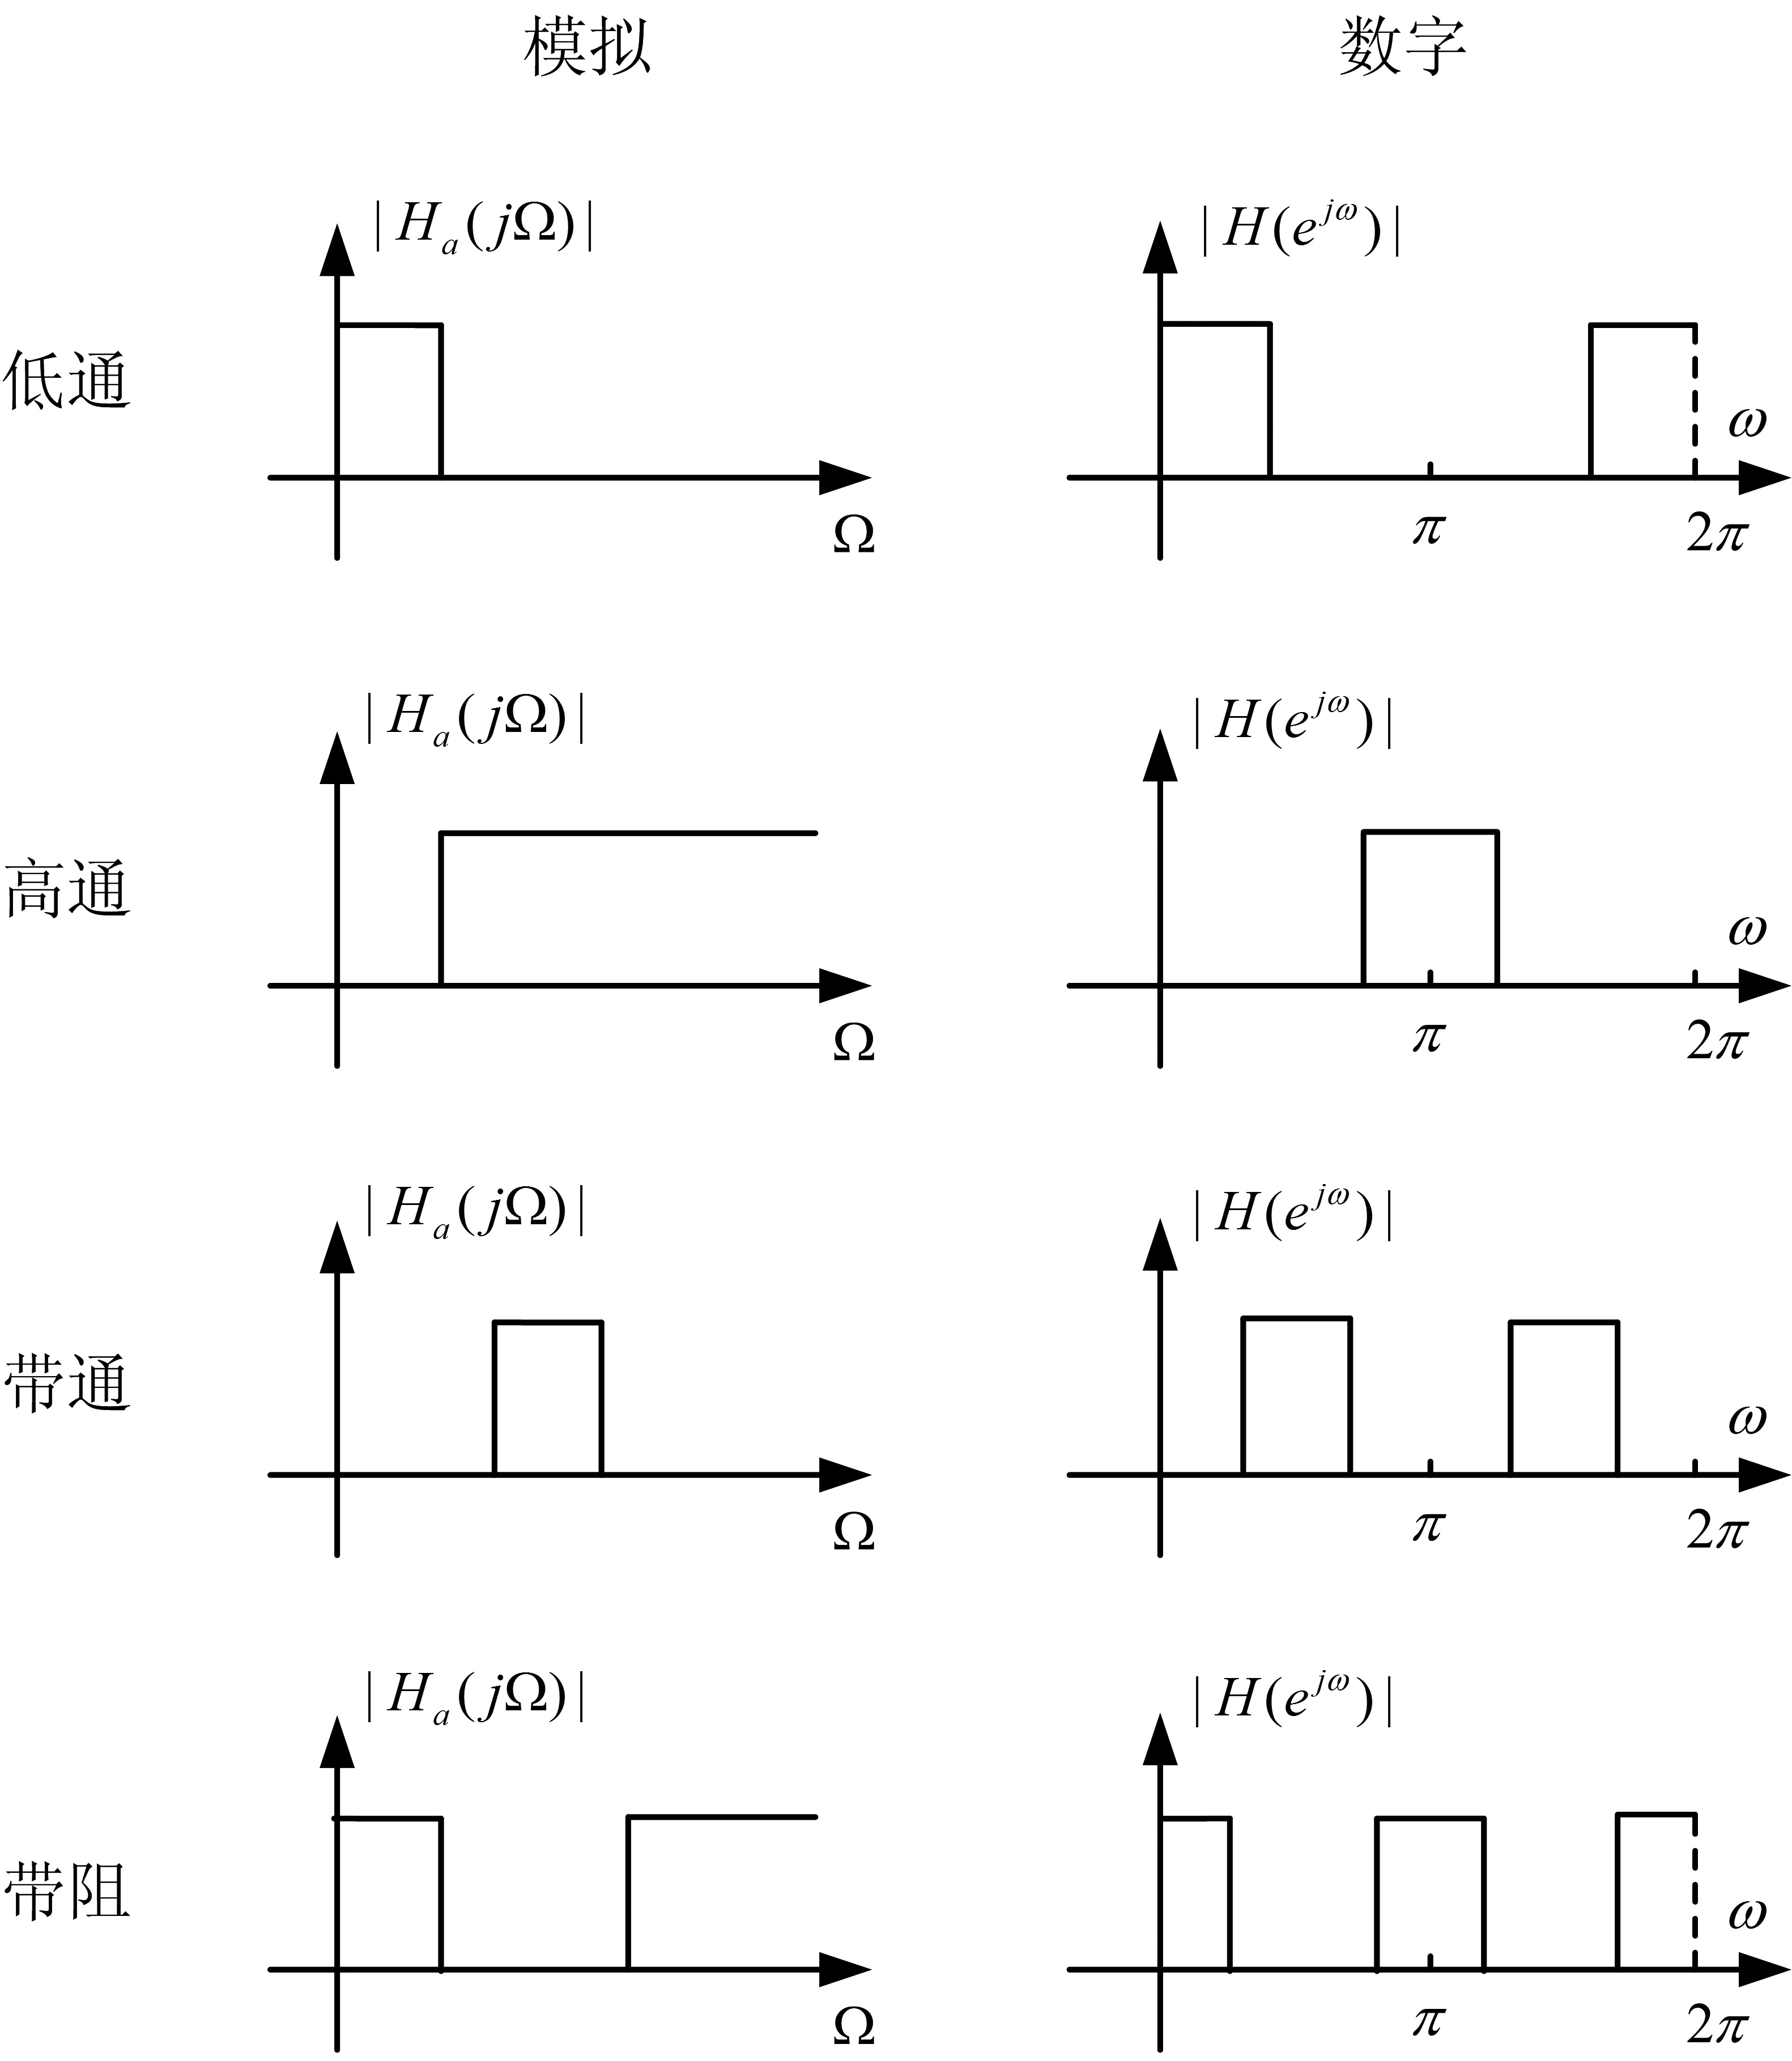
\includegraphics[width=0.8\textwidth]{fig4dtgtdtdz.jpg}
%\caption{不同类型选频滤波器的幅频特性}
\end{figure}
\end{frame}
\subsection{6.1.4 数字滤波器的设计}
%%%%%%%%%%%%%%%%%%%%%%%%%%%%%%%%%%%%%%%%%%%%%%%%%%%%%%%%%%%%%%%%%%%%%%%%%%%%%%%%%%%%%%%%%%%%%%%
\begin{frame}\frametitle{}%[allowframebreaks]
\textbf{\heiti 四、数字滤波器的设计}
\newline

1、直接法(不讲)
\begin{enumerate}
\item [(1)] 在时域中设计
\item [(2)] 在频域中设计
\end{enumerate}
2、从AF设计DF
\begin{enumerate}
\item [(1)]  根据$DF$技术指标要求设计模拟滤波器,得到$H_{a}(s)$(6.2节)
\item [(2)] 利用一种映射方法,将    $$H_{a}(s)\underrightarrow{\quad\quad\mbox{映射为}\quad\quad}
{\quad\quad}H(z)$$
映射方法
\begin{enumerate}
\item [(a)] 脉冲响应不变法 \quad (6.3节)
\item [(b)] 双线性变换法  \qquad (6.4节)
\end{enumerate}
\end{enumerate}
\end{frame}
%%%%%%%%%%%%%%%%%%%%%%%%%%%%%%%%%%%%%%%%%%%%%%%%%%%%%%%%%%%%%%%%%%%%%%%%%%%%%%%%%%%%%%%%%%%%%%
\section{6.2 模拟滤波器的设计方法}
\subsection{6.2.1 模拟低通滤波器的设计}
%%%%%%%%%%%%%%%%%%%%%%%%%%%%%%%%%%%%%%%%%%%%%%%%%%%%%%%%%%%%%%%%%%%%%%%%%%%%%%%%%%%%%%%%%%%%%%
\begin{frame}\frametitle{}%[allowframebreaks]6.2 模拟滤波器的设计方法
%\textbf{一、模拟选频滤波器}
\textbf{\heiti 一、模拟选频滤波器的概念}
\begin{enumerate}
       \item 模拟选频滤波器
        \begin{figure}[h]
            \centering
        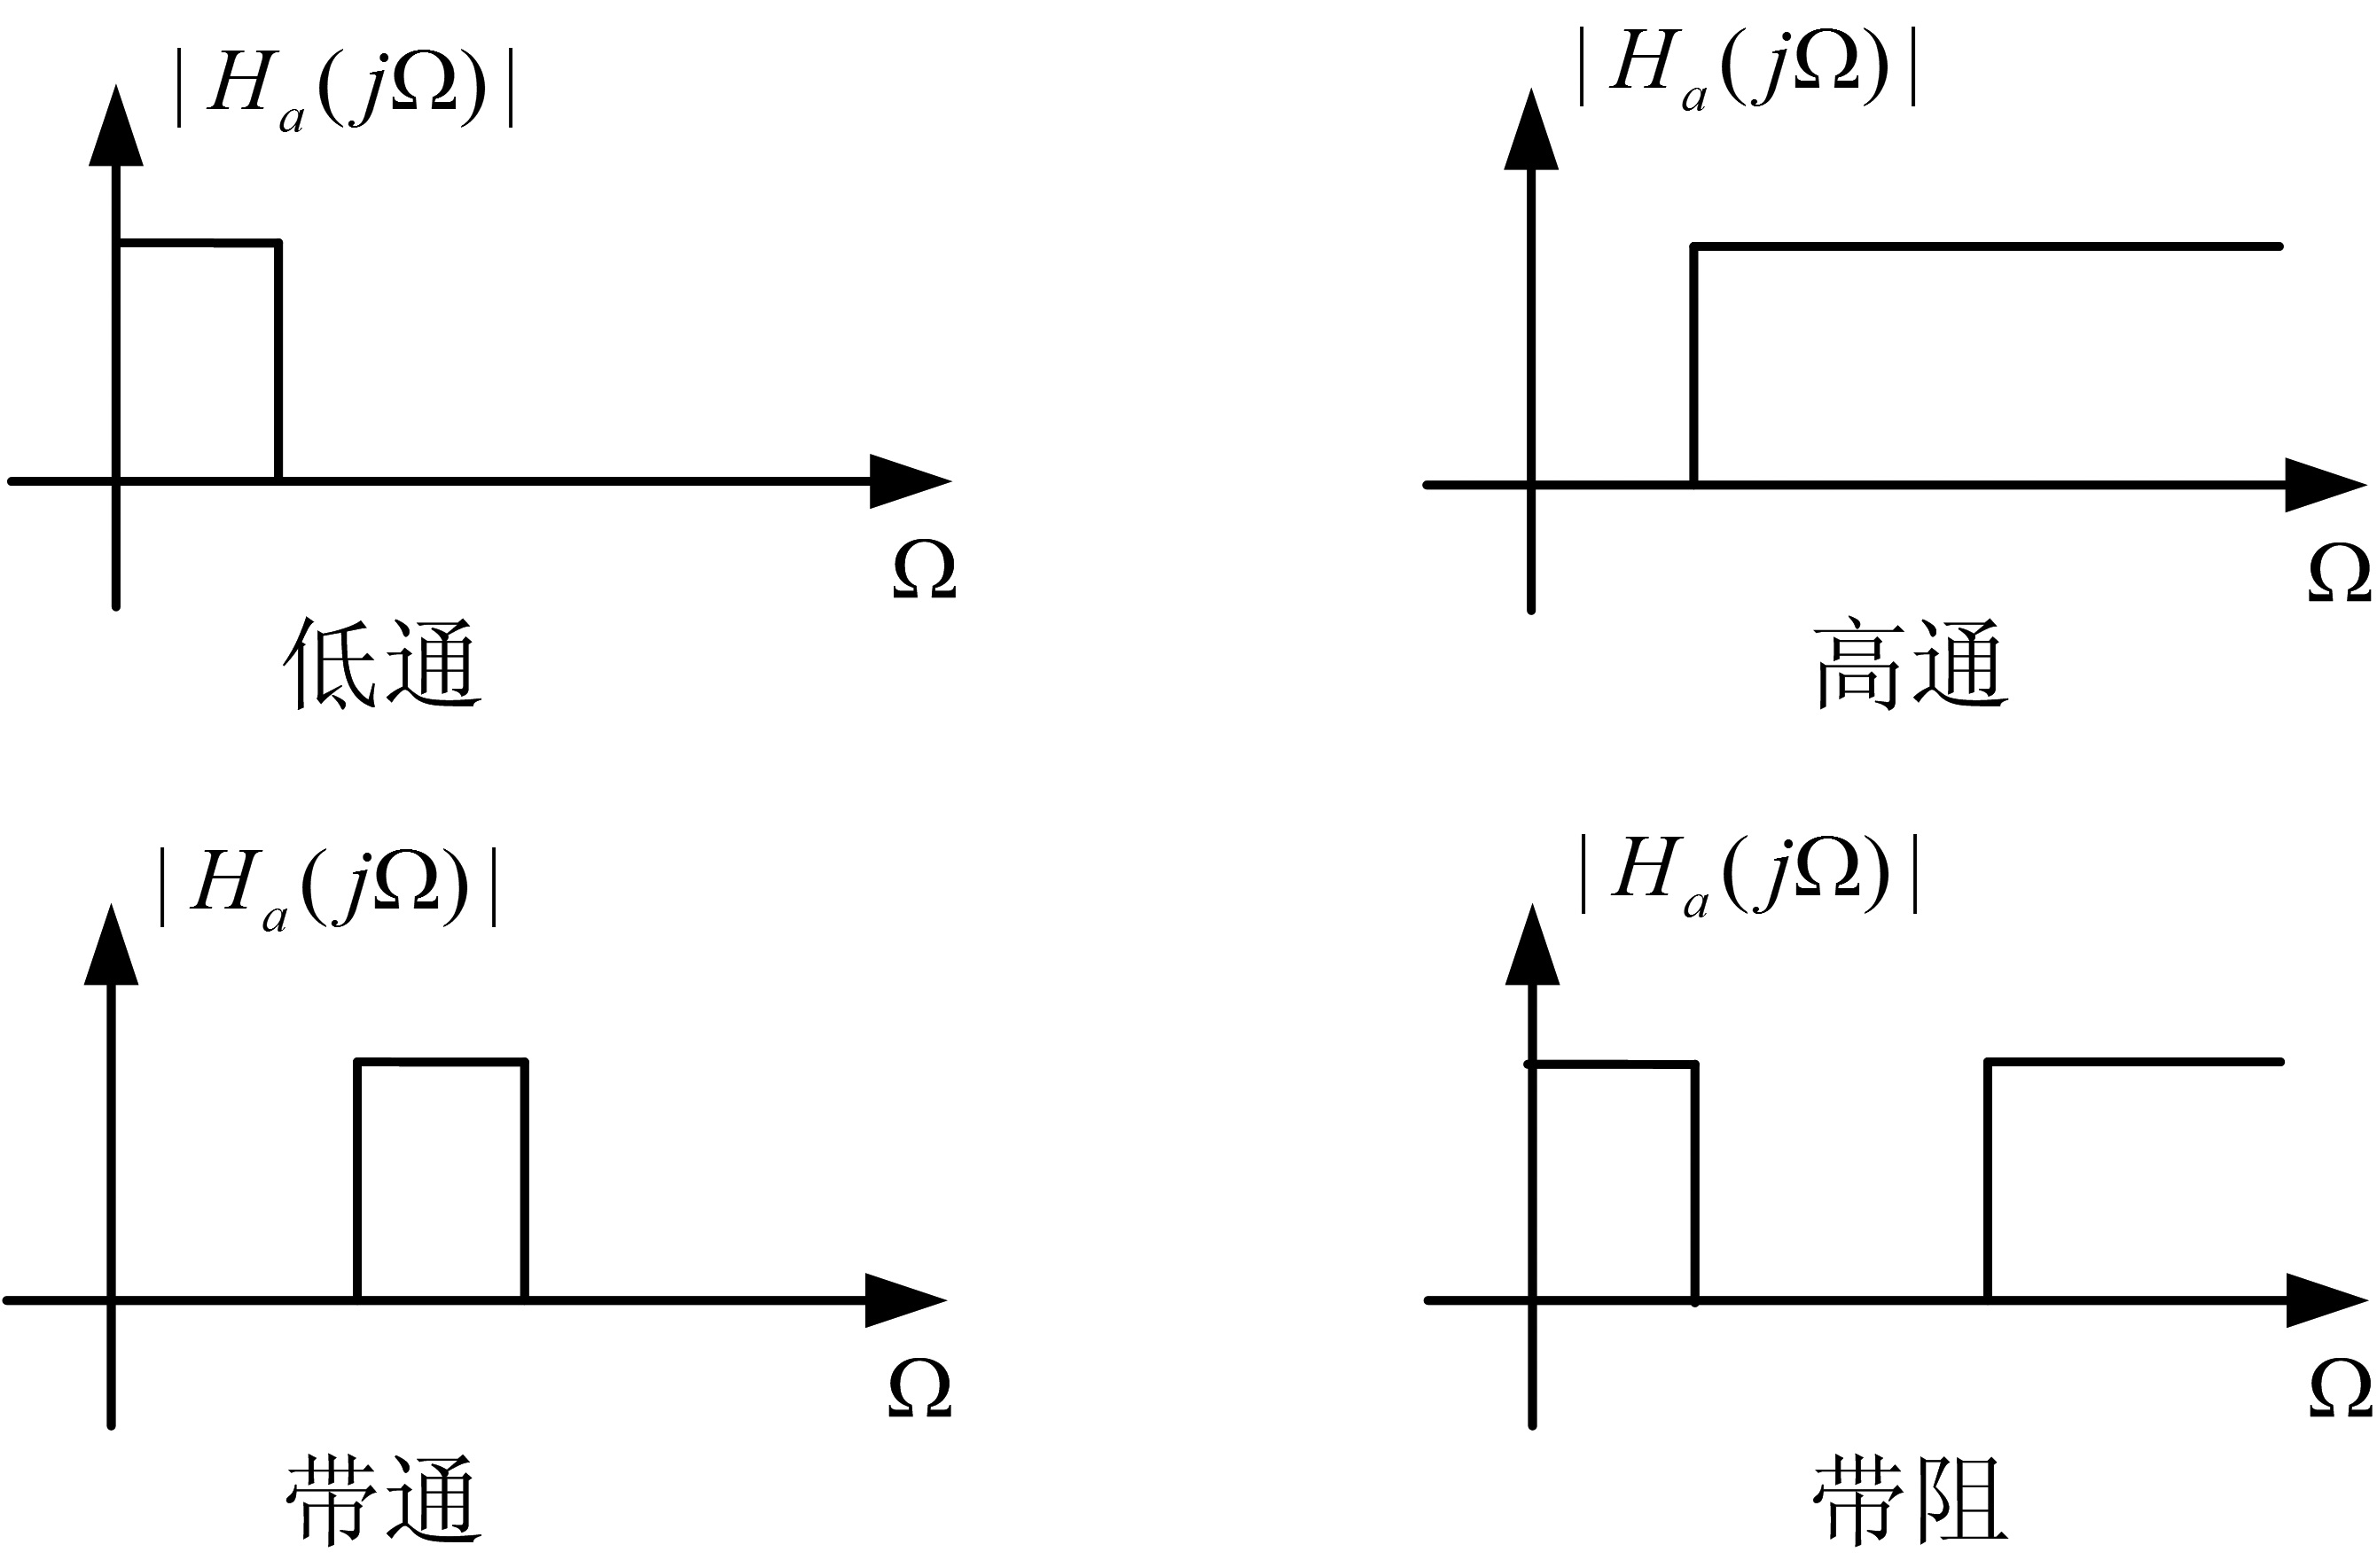
\includegraphics[width=0.6\textwidth]{fig5_mndtgtdtdz.jpg}
        %\caption{模拟选频滤波器图}
        \end{figure}
       \item
       低通滤波器的设计是关键,其他滤波器可通过频率变换,将低通滤波器转换
       为相应的模拟滤波器。
\end{enumerate}
\end{frame}
%%%%%%%%%%%%%%%%%%%%%%%%%%%%%%%%%%%%%%%%%%%%%%%%%%%%%%%%%%%%%%%%%%%%%%%%%%%%%%%%%%%%%%%%%%%%%%
\begin{frame}[shrink]\frametitle{}%[allowframebreaks]

\textbf{\heiti 二、设计方法(逼近法)}

\begin{enumerate}
      \item  [1]  理想滤波器无法用模拟滤波器实现
          \begin{enumerate}
            \item [(1)] 实际工作中,用实际滤波器$\quad\underrightarrow{\quad\mbox{逼近}
                \quad}\quad$理想滤波器。
            \item [(2)] 当所涉及的实际滤波器满足技术要求时,停止逼近。
          \end{enumerate}
          \par\quad%\newline
      \item  [2]   假设滤波器的响应函数为$H_{a}(j\Omega)$\quad (或$H_{a}(s)$)
          \par
%             显然有\quad\quad
%             $$H_{a}(s)= LT[h_{a}(t)] = \int_{-\infty}^{\infty}h_{a}(t)e^{-st}dt $$
%             $$H_{a}(j\Omega)= FT[h_{a}(t)] = \int_{-\infty}^{\infty}h_{a}(t)e^{-j\Omega t}dt$$
               \begin{itemize}
                 \item [(1)]设计指标由$|H_{a}(j\Omega)|$给出。
                     \begin{itemize}
                       \item 对于典型的滤波器,其相频特性是确定的
                     \end{itemize}

                 \item [(2)]滤波器由$H_{a}(s)$给出。
                     \begin{itemize}
                       \item 注意$h_a(t),H_a(j\Omega),H_a(s)$是对系统的等价描述
                     \end{itemize}
               \end{itemize}
\begin{dablock}
问题在于:
$$\mbox{如何由}\quad\quad \left|H_{a}(j\Omega)\right| \longrightarrow H_{a}(s)$$
\quad\newline\quad
\end{dablock}
\end{enumerate}
\end{frame}
%%%%%%%%%%%%%%%%%%%%%%%%%%%%%%%%%%%%%%%%%%%%%%%%%%%%%%%%%%%%%%%%%%%%%%%%%%%%%%%%%%%%%%%%%%%%%%
%%%%%%%%%%%%%%%%%%%%%%%%%%%%%%%%%%%%%%%%%%%%%%%%%%%%%%%%%%%%%%%%%%%%%%%%%%%%%%%%%%%%%%%%%%%%%%
\begin{frame}[allowframebreaks]\frametitle{}%[allowframebreaks]
\textbf{\heiti 三、实因果系统传输函数的设计}\\
\quad\\
\textbf{对于实因果系统,如何由$|H_a(j\Omega)|^2$得到$H_a(s)$。}

\quad\\
\begin{enumerate}
  \item [1] 特点:
      设某因果系统,$h_a(t)$为实函数,有:
      \begin{equation*} 
        \begin{split}
        H_{a}(j\Omega)&= FT[H_{a}(t)] = \int_{-\infty}^{\infty}h_{a}(t)e^{-j\Omega t}dt \\
         H_{a}(j\Omega)&=|H_{a}(j\Omega)|\cdot e^{jarg[H_{a}(j\Omega)]}\\
        \end{split}
      \end{equation*}
%      \quad\\
%      \quad\\
%      \quad\\
%      \quad\\
\begin{zhuyi}
\quad\qquad      注意: 此处,$H_a(j\Omega)$与$H_a(s)$可相互等价
\end{zhuyi}
   \newpage

      \textbf{重要结论(自证)}
      \begin{enumerate}
%        \item [(1)] $|H_{a}(j\Omega)|$ 是$\Omega$ 的偶函数。
%        \item [(2)] $arg[H_{a}(j\Omega)]$是$\Omega$ 的奇函数。
        \item  幅度平方函数  $\quad |H_{a}(s)|^{2}=H_{a}(s)H_{a}(-s)$
            $$|H_{a}(j\Omega)|^{2}=H_{a}(j\Omega)H_{a}(-j\Omega)\quad\quad\quad\quad\quad\quad\quad\quad\quad\quad\quad$$
            $$\quad |H_{a}(s)|^{2}=H_{a}(s)H_{a}(-s)  \quad\quad\quad\quad   \left(H_{a}(j\Omega)= H_{a}(s)|_{s=\j\Omega}\right)$$
            \textbf{说明:}
            $$|H_{a}(s)|^{2}=H_{a}(s)H_{a}^{*}(s)      \quad\quad\quad \mbox{只需证:}\quad\quad    H_{a}(-s)=H_{a}^{*}(s)  $$

      \end{enumerate}



  \item [2]  由
            \quad $|H_{a}(s)|^{2}\rightarrow H_{a}(s)$
            %\par(注:$H_{a}(j\Omega)= H_{a}(s)|_{s=\j\Omega}$)
            %$|H_{a}(j\Omega)|^{2}\rightarrow H_{a}(j\Omega)\quad$
            \newline
            \par 假设$|H_{a}(s)|^{2}$是{\heiti 全极点函数},有$2N$个极点,则可由幅度平方函数$|H_{a}(j\Omega)|^{2}$求出系统函数。

%      \texttt{分析:}
%        $$|H_a(s)|^{2} = H_a(s)H_a(-s)$$
%        \begin{enumerate}
%          \item [(1)]设$s_{k}$是$H_a(s)$的任意一个极点,则$-s_{k}$是$H_a(-s)$的一个极点。
%          $$ H(s_{k})=\infty\quad\quad \rightarrow \quad\quad H(-(-s_{k}))=\infty$$
%             $\therefore$ $-s_{k}$ 为 $H_a(-s)$ 的极点,极点关于原点对称。
%          \item [(2)]如$H_a(s)$有N个极点,$H_a(-s)$有N个极点,则$|H_a(s)|^{2}$有2N个极点。
%          \item [(3)]2N个极点中,S平面左右半平面各有一半。
%          \item [(4)]设系统因果稳定,则:
%            $$
%                \left\{ \begin{aligned}
%                \mbox{ } & \mbox{$H_a(s)$的$N$个极点全部在$S$的左半平面。} \quad\quad\quad\quad\quad\quad\quad\quad\quad\quad\quad\quad\\
%                \mbox{ } & \mbox{$H_a(-s)$的$N$个极点全部在$S$的右半平面。}
%                \end{aligned} \right.
%            $$
%            可由S左半平面的N个极点构造出$H_a(s)$.
%        \end{enumerate}
\end{enumerate}
\end{frame}
%%%%%%%%%%%%%%%%%%%%%%%%%%%%%%%%%%%%%%%%%%%%%%%%%%%%%%%%%%%%%%%%%%%%%%%%%%%%%%%%%%%%%%%%%%%%%%
\begin{frame}\frametitle{}%[allowframebreaks]
\texttt{分析:}
        $$|H_a(s)|^{2} = H_a(s)H_a(-s)$$
        \begin{enumerate}
          \item [(1)]设$s_{k}$是$H_a(s)$的任意一个极点,则$-s_{k}$是$H_a(-s)$的一个极点。
          $$ H(s_{k})=\infty\quad\quad \rightarrow \quad\quad H(-(-s_{k}))=\infty$$
             $\therefore$ $-s_{k}$ 为 $H_a(-s)$ 的极点,极点关于原点对称。
          \item [(2)]如$H_a(s)$有N个极点,$H_a(-s)$有N个极点,则$|H_a(s)|^{2}$有2N个极点。
          \item [(3)]2N个极点中,S平面左右半平面各有一半。
          \item [(4)]设系统$H_a(s)$因果稳定,则:
            $$
                \left\{ \begin{aligned}
                \mbox{ } & \mbox{$H_a(s)$的$N$个极点全部在$S$的左半平面。} \quad\quad\quad\quad\quad\quad\quad\quad\quad\quad\quad\quad\\
                \mbox{ } & \mbox{$H_a(-s)$的$N$个极点全部在$S$的右半平面。}
                \end{aligned} \right.
            $$
            可由S左半平面的N个极点构造出$H_a(s)$.
        \end{enumerate}
%\end{enumerate}
\end{frame}

%%%%%%%%%%%%%%%%%%%%%%%%%%%%%%%%%%%%%%%%%%%%%%%%%%%%%%%%%%%%%%%%%%%%%%%%%%%%%%%%%%%%%%%%%%%%%%

\subsection{6.2.2 模拟低通滤波器的技术要求及逼近方法}

\subsubsection*{LP-AF的技术要求(技术指标)}

%%%%%%%%%%%%%%%%%%%%%%%%%%%%%%%%%%%%%%%%%%%%%%%%%%%%%%%%%%%%%%%%%%%%%%%%%%%%%%%%%%%%%%%%%%%%%%
\begin{frame}\frametitle{LP-AF的技术要求}%[allowframebreaks]
{\heiti 一、LP-AF的技术要求(技术指标)}
\begin{figure}[h]
  \centering
  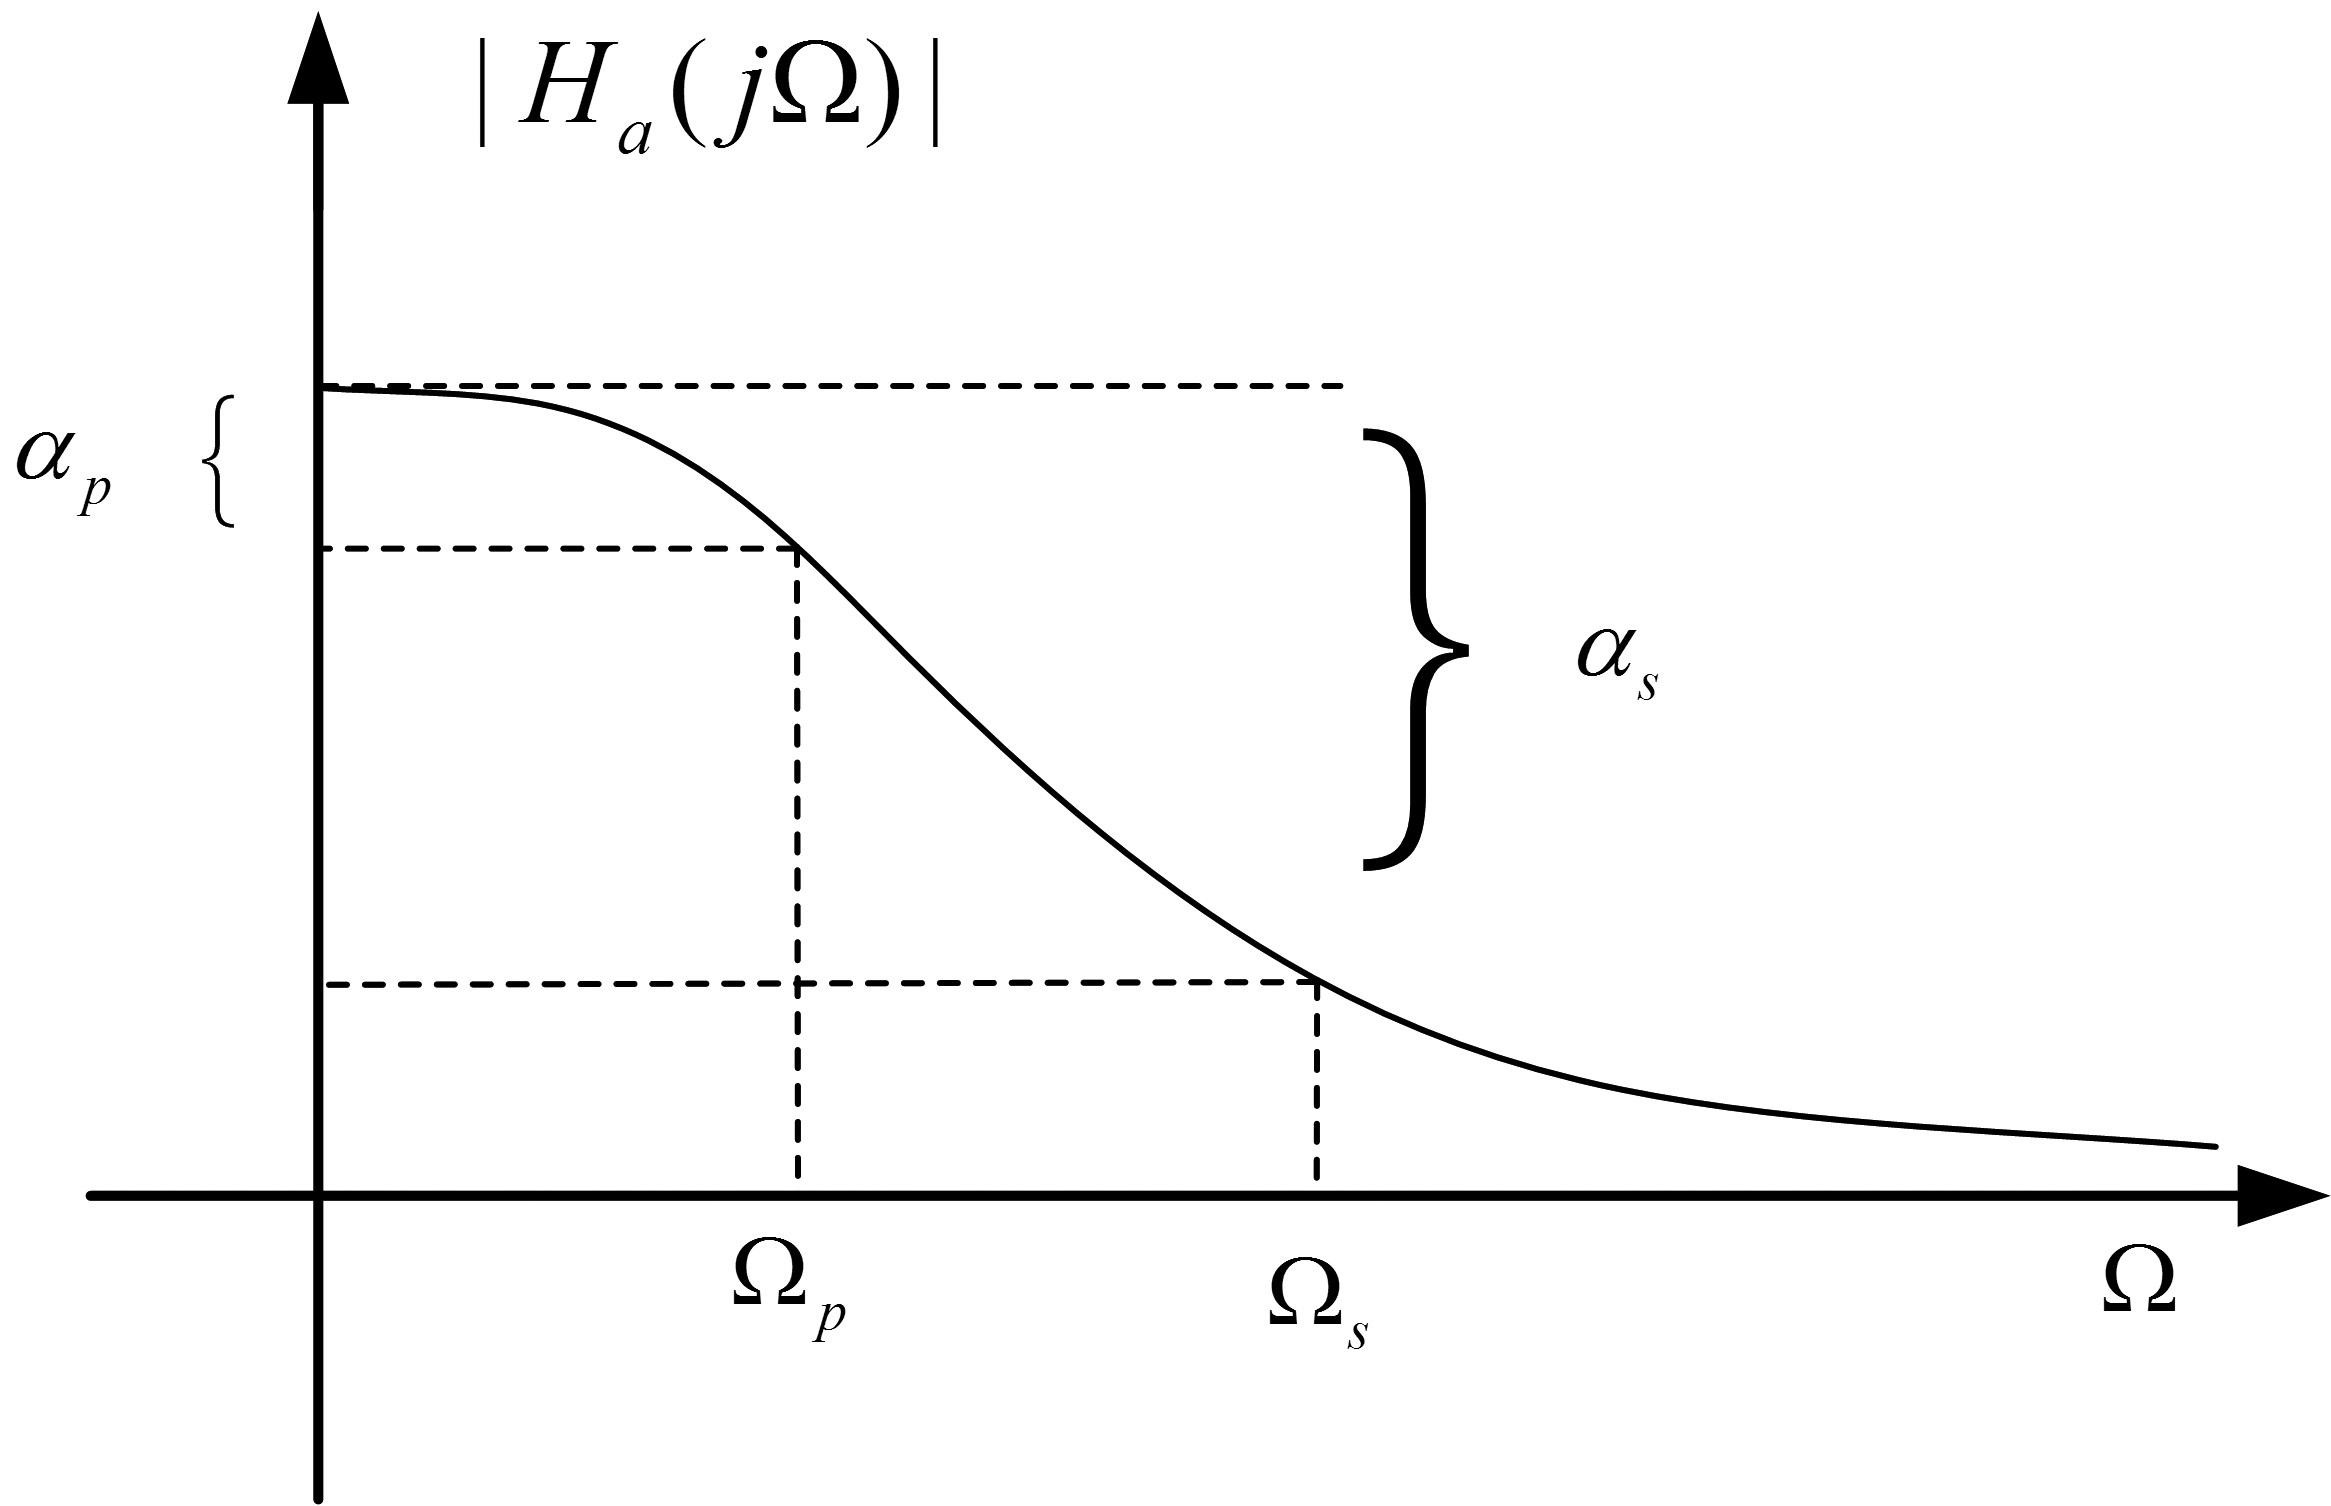
\includegraphics[width=0.55\textwidth]{fig6_lpafjszb.jpg}
\end{figure}
两对参数即可得到模拟滤波器的形状,也叫做片段常数特性。
\begin{enumerate}
  \item $\Omega_{p}$:通带边界频率
  \item $\alpha_{p}$:通带允许的最大衰减
  \item $\Omega_{s}$:阻带截止频率
  \item $\alpha_{s}$:阻带内允许的最小衰减
\end{enumerate}
\end{frame}
%%%%%%%%%%%%%%%%%%%%%%%%%%%%%%%%%%%%%%%%%%%%%%%%%%%%%%%%%%%%%%%%%%%%%%%%%%%%%%%%%%%%%%%%%%%%%%


%%%%%%%%%%%%%%%%%%%%%%%%%%%%%%%%%%%%%%%%%%%%%%%%%%%%%%%%%%%%%%%%%%%%%%%%%%%%%%%%%%%%%%%%%%%%%%
\begin{frame}\frametitle{}%[allowframebreaks]
\begin{enumerate}
\item [1]关于衰减的说明:
$$\mbox{有:}\quad\quad\quad\quad
\alpha(\Omega) = 10 lg\left(\frac{1}{|H_{a}(j\Omega)|^{2}}\right)= - 10 lg\left|H_{a}(j\Omega)\right|^{2}$$
\emph{ 简单证明:}
$$\alpha(\Omega)
= -20 lg\left(\frac{|H_{a}(j\Omega)|}{|H_{a}(j0)|}\right)\quad\quad$$
设$\quad\quad\quad\quad|H_{a}(j0)|=1 $
$$\mbox{则:}\quad\quad\alpha(\Omega)= 10 lg(\frac{1}{|H_{a}(j\Omega)|^{2}})
\quad\quad\mbox{(单位为$dB$)}$$
\end{enumerate}
\end{frame}
%%%%%%%%%%%%%%%%%%%%%%%%%%%%%%%%%%%%%%%%%%%%%%%%%%%%%%%%%%%%%%%%%%%%%%%%%%%%%%%%%%%%%%%%%%%%%%


%%%%%%%%%%%%%%%%%%%%%%%%%%%%%%%%%%%%%%%%%%%%%%%%%%%%%%%%%%%%%%%%%%%%%%%%%%%%%%%%%%%%%%%%%%%%%%
\begin{frame}[shrink]\frametitle{}%[allowframebreaks]

\begin{enumerate}
\item [2] 3dB截止频率$\Omega_{c}$\par

\par\quad

即当$|H_{a}(j\Omega)|$下降到零频分量的$\frac{\sqrt{2}}{2}$时对应的频率为$\Omega_{c}$,此时衰减约为$3dB$
$$\alpha(\Omega_{c})\thickapprox 3dB \quad\quad\Rightarrow\quad\quad
\frac{\big|H_{a}(j\Omega_{c})\big|}{\big|H_{a}(j0)\big|} = \frac{\sqrt{2}}{2} = 0.707$$
\emph{注意:}
    \begin{itemize}
        \item 事实上$\alpha(\Omega_{c})=10\cdot lg2 \approx 3.0103$,是约等于3。
        \item 另,$\Omega_{c}$与$\Omega_{p}$是不同的概念。
    \end{itemize}
\end{enumerate}

\end{frame}
%%%%%%%%%%%%%%%%%%%%%%%%%%%%%%%%%%%%%%%%%%%%%%%%%%%%%%%%%%%%%%%%%%%%%%%%%%%%%%%%%%%%%%%%%%%%%%


%%%%%%%%%%%%%%%%%%%%%%%%%%%%%%%%%%%%%%%%%%%%%%%%%%%%%%%%%%%%%%%%%%%%%%%%%%%%%%%%%%%%%%%%%%%%%%
\begin{frame}\frametitle{}%[allowframebreaks]
{\heiti 二、Butterworth逼近方法}
    \par\par\par 设$H_{d}(s)$是理想滤波器
\begin{enumerate}
   \item [1]
       \par\par\par 任务:

       设计一个实际的LP-AF,得到其系统函数$H_{a}(s)$,
       使得$|H_{a}(s)|\underrightarrow{\mbox{\quad 逼近\quad}}|H_{d}(s)|$
   \item [2] 具体思路:
        \begin{enumerate}
          \item [(1)] 用幅度平方函数作为逼近函数,即:
                    $$|H_{a}(s)|^{2}\underrightarrow{\quad\mbox{逼近}\quad} |H_{d}(s)|^{2}$$
          \item [(2)]逼近函数的表达式:
                    $$\left|H_{a}(j\Omega)\right|^2= \frac{1}{1+|k(j\Omega)|^{2}}$$
                    其中$|k(j\Omega)|^{2}$是以$\Omega^{2}$为自变量的N次有理多项式。
          \item [(3)] $|H_{a}(j\Omega)|^{2}\underrightarrow{\mbox{\quad 得到 \quad}} H_{a}(j\Omega)(\mbox{或}H_{a}(s))$
    \end{enumerate}
\end{enumerate}
\end{frame}
%%%%%%%%%%%%%%%%%%%%%%%%%%%%%%%%%%%%%%%%%%%%%%%%%%%%%%%%%%%%%%%%%%%%%%%%%%%%%%%%%%%%%%%%%%%%%%
\subsection{6.2.3 最平响应Butterworth Filter设计}

%%%%%%%%%%%%%%%%%%%%%%%%%%%%%%%%%%%%%%%%%%%%%%%%%%%%%%%%%%%%%%%%%%%%%%%%%%%%%%%%%%%%%%%%%%%%%%
\begin{frame}[shrink]\frametitle{最平响应Butterworth系统}%[allowframebreaks]

\textbf{\heiti 一、最平响应Butterworth系统}
$$|H_{a}(j\Omega)|^{2}= \frac{1}{1+C^{2}\Omega^{2N}}$$
$$  \mbox{两个未知参数C,N,确定之即可得$|H_{a}(j\Omega)|^{2}$} $$
\end{frame}
%%%%%%%%%%%%%%%%%%%%%%%%%%%%%%%%%%%%%%%%%%%%%%%%%%%%%%%%%%%%%%%%%%%%%%%%%%%%%%%%%%%%%%%%%%%%%%


%%%%%%%%%%%%%%%%%%%%%%%%%%%%%%%%%%%%%%%%%%%%%%%%%%%%%%%%%%%%%%%%%%%%%%%%%%%%%%%%%%%%%%%%%%%%%%
\begin{frame}[allowframebreaks]\frametitle{最平响应Butterworth滤波器设计}%[allowframebreaks]
\begin{enumerate}
  \item  [(1)] 得到$|H_{a}(j\Omega)|^2$
  \par  将$|H_{a}(j\Omega)|^{2}$代入衰减函数:
  $$\alpha(\Omega) = 10 lg(\frac{1}{|H_{a}(j\Omega)|^{2}})$$
  代入,得:
  $$\alpha(\Omega) = 10 lg(1+C^{2}\Omega^{2N})$$
  变换后可得:
  $$1+C^{2}\Omega^{2N}=10^{\frac{\alpha(\Omega)}{10}}
  \mbox{\quad\quad(可证明$C=\frac{1}{\Omega_{c}^{N}})$}$$
  \newpage
  即:
  $$\quad 1+(\frac{\Omega}{\Omega_{c}})^{2N}=10^{
    \frac{\alpha(\Omega)}{10}}
    \quad\quad\quad\quad\quad\quad$$
  我们知道,LP-AF由两对参数决定,即:
    $$
    \left\{
    \begin{aligned}
    \mbox{$\Omega_{p}$:} &\quad \mbox{通带边界频率} \quad\quad\quad\quad\quad\quad\quad\quad\quad\quad\quad\quad\\
    \mbox{$\alpha_{p}$:} &\quad \mbox{通带允许的最大衰减}
    \end{aligned}
    \right.
    $$
    $$
    \left\{
    \begin{aligned}
    \mbox{$\Omega_{s}$:} &\quad \mbox{阻带截止频率} \quad\quad\quad\quad\quad\quad\quad\quad\quad\quad\quad\quad\\
    \mbox{$\alpha_{s}$:} &\quad \mbox{阻带内允许的最小衰减}
    \end{aligned}
    \right.
    $$
%    $$\mbox{则:}\quad\quad 1+C^{2}\Omega^{2N}=10^{\frac{\alpha(\Omega)}{10}}
%     \quad\quad\quad\quad\quad\quad\quad\quad$$
     \newpage
    $$\mbox{对右边方程:}\quad 1+(\frac{\Omega}{\Omega_{c}})^{2N}=10^{
    \frac{\alpha(\Omega)}{10}}
    \quad\quad\quad\quad\quad\quad\quad\quad\quad\quad\quad$$

    代入$(\Omega_{p},\alpha_{p})$,$(\Omega_{s}\alpha_{s})$后可得:
    $$
    \left\{ \begin{aligned}
        1+\left(\frac{\Omega_{p}}{\Omega_{c}}\right)^{2N} &= 10^{\frac{\alpha_{p}}{10}}\\
        1+\left(\frac{\Omega_{s}}{\Omega_{c}}\right)^{2N} &= 10^{\frac{\alpha_{s}}{10}}
        \quad\quad\quad\quad\quad\quad\quad\quad\\
    \end{aligned} \right.
    $$
    两个方程,两个未知数,联立求解后可得$\Omega_{c}$,$N$。
    最后可得:
    $$|H_{a}(j\Omega)|^{2}= \frac{1}{1+(\frac{\Omega}{\Omega_{c}})^{2N}}$$
    \newpage
    \textbf{说明}
    \begin{enumerate}
      \item 算法相当简单,结果好。
      \item N与幅频特性函数$H_{a}(j\Omega)$的关系:N越大,形状越好。
        \begin{figure}[h]
          \centering
          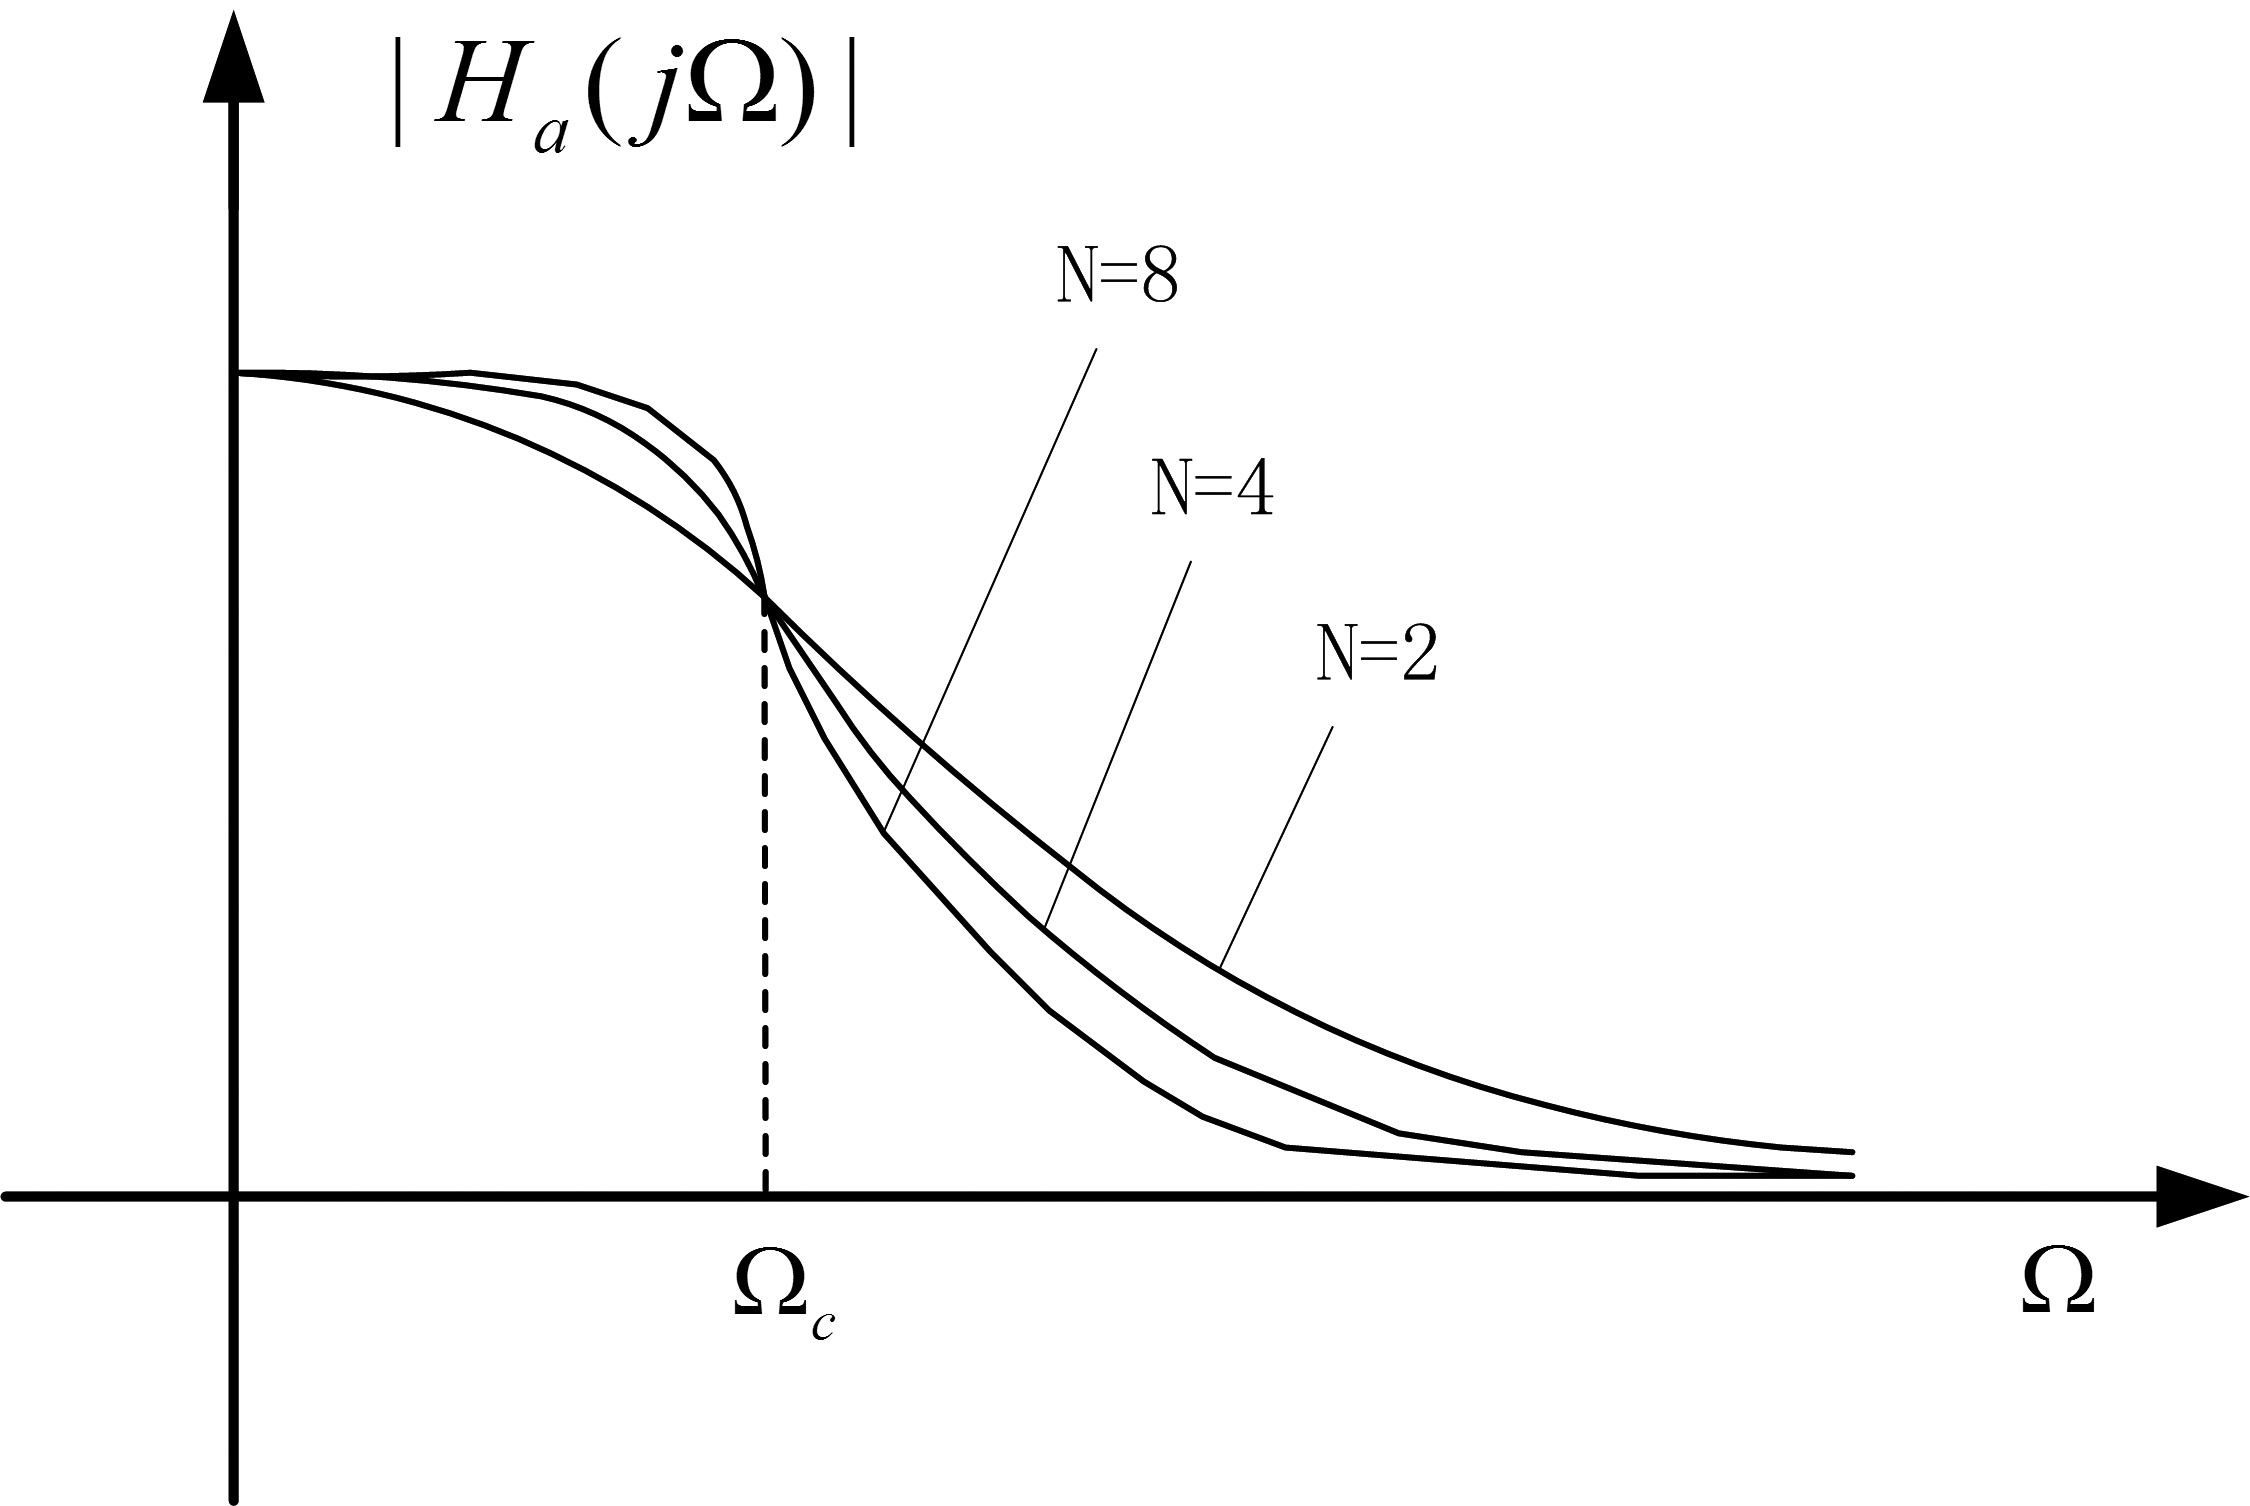
\includegraphics[width=0.5\textwidth]{fig7_btwsdtfdtx.jpg}
        \end{figure}
    \end{enumerate}
    \end{enumerate}
\end{frame}
%%%%%%%%%%%%%%%%%%%%%%%%%%%%%%%%%%%%%%%%%%%%%%%%%%%%%%%%%%%%%%%%%%%%%%%%%%%%%%%%%%%%%%%%%%%%%%


%%%%%%%%%%%%%%%%%%%%%%%%%%%%%%%%%%%%%%%%%%%%%%%%%%%%%%%%%%%%%%%%%%%%%%%%%%%%%%%%%%%%%%%%%%%%%%
\begin{frame}[allowframebreaks]\frametitle{}%[allowframebreaks]
\begin{enumerate}
  \item  [(2)] $\quad\quad\quad\quad\quad
      |H_{a}(s)|^{2}\underrightarrow{\quad\mbox{求得}\quad}H_{a}
      (j\Omega)\quad\quad(\mbox{或$H_a(s)$})$
       $$|H_{a}(j\Omega)|^{2}= \frac{1}{1+(\frac{\Omega}{\Omega_{c}})^{2N}}$$
      令$s=j\Omega$,则有:
      $$|H_{a}(s)|^{2}= \frac{1}{1+(\frac{s}{j\Omega_{c}})^{2N}}   =\frac{(j\Omega_{c})^{2N}}{s^{2N}+(j\Omega_{c})^{2N}}$$
      令分母为0,即$s^{2N}+(j\Omega_{c})^{2N}=0$,求极点。 有:
      $$s^{2N}=-(j\Omega_{c})^{2N}= e^{j(2k+1)\pi}(j\Omega_{c})^{2N}\quad   \quad k=0,1,...,(2N-1)$$
      $$s_{k}= e^{j\frac{(2k+1)}{2N}\pi}\cdot j\cdot \Omega_{c}\quad\quad   \mbox{注意$j=e^{j\frac{\pi}{2}}$} $$
      整理后有:
      $$s_{k}=\Omega_{c}\cdot e^{j\pi[\frac{1}{2}+\frac{2k+1}{2N}]}
      \quad\quad k=0,1,...,(2N-1)$$
      2N个极点等间隔分布在半径为$\Omega_{c}$的圆上。
      \par (该圆也叫Butterworth圆)


      前述已知:
      \begin{dablock}
      $$|H_{a}(s)|^{2}=H_{a}(s)\cdot H_{a}(-s)$$
      \par \quad\quad $|H_{a}(s)|^{2}$有2N个极点,且左右半平面各一半,其中:
      $$
        \left\{
        \begin{aligned}
        \mbox{\quad$H_{a}(s)$}&\quad \mbox{的N个极点全在左半平面;}\\
        \mbox{$H_{a}(-s)$}&\quad \mbox{的N个极点全在右半平面。}\\
        \end{aligned}
        \right.
      $$
      \end{dablock}
      则
      $s_{k}=\Omega_{c}\cdot e^{j\pi[\frac{1}{2}+\frac{2k+1}{2N}]}$
      的前N个极点全在S左半平面内。
     % \begin{dablock}
  \end{enumerate}
\end{frame}

%%%%%%%%%%%%%%%%%%%%%%%%%%%%%%%%%%%%%%%%%%%%%%%%%%%%%%%%%%%%%%%%%%%%%%%%%%%%%%%%%%%%%%%%%%%%%%


%%%%%%%%%%%%%%%%%%%%%%%%%%%%%%%%%%%%%%%%%%%%%%%%%%%%%%%%%%%%%%%%%%%%%%%%%%%%%%%%%%%%%%%%%%%%%%
\begin{frame}\frametitle{举例说明,以N=4为例}%[allowframebreaks]
举例说明,以N=4为例:
      $$
        \left\{
        \begin{aligned}
        \mbox{$k=0,$} &\quad\quad\quad\quad\mbox{$s_{0}= \Omega_{c}\cdot e^{j\frac{5}{8}\pi}$}\quad\quad\quad\quad\quad\quad\quad\quad\\
        \mbox{$k=1,$} &\quad\quad\quad\quad\mbox{$s_{1}= \Omega_{c}\cdot e^{j\frac{7}{8}\pi}$}\\
        \end{aligned}
        \right.
      $$
      $$
        \left\{
        \begin{aligned}
        \mbox{$k=2,$} &\quad\quad\quad\quad\mbox{$s_{2}= \Omega_{c}\cdot e^{j\frac{9}{8}\pi}$}\quad\quad\quad\quad\quad\quad\quad\quad\\
        \mbox{$k=3,$} &\quad\quad\quad\quad\mbox{$s_{3}= \Omega_{c}\cdot e^{j\frac{11}{8}\pi}$}\\
        \end{aligned}
        \right.
      $$
      $$
        \left\{
        \begin{aligned}
        \mbox{$k=4,$} &\quad\quad\quad\quad\mbox{$s_{4}= \Omega_{c}\cdot e^{j\frac{13}{8}\pi}$}\quad\quad\quad\quad\quad\quad\quad\quad\\
        \mbox{$k=5,$} &\quad\quad\quad\quad\mbox{$s_{5}= \Omega_{c}\cdot e^{j\frac{15}{8}\pi}$}\\
        \end{aligned}
        \right.
      $$
      $$
        \left\{
        \begin{aligned}
        \mbox{$k=6,$} &\quad\quad\quad\quad\mbox{$s_{6}= \Omega_{c}\cdot e^{j\frac{1}{8}\pi}$}\quad\quad\quad\quad\quad\quad\quad\quad\\
        \mbox{$k=7,$} &\quad\quad\quad\quad\mbox{$s_{7}= \Omega_{c}\cdot e^{j\frac{3}{8}\pi}$}\\
        \end{aligned}
        \right.
      $$
      \end{frame}
      %\newpage
\begin{frame}\frametitle{}%[allowframebreaks]
      极点分布图如下图所示:
      \begin{figure}[h]
          \centering
          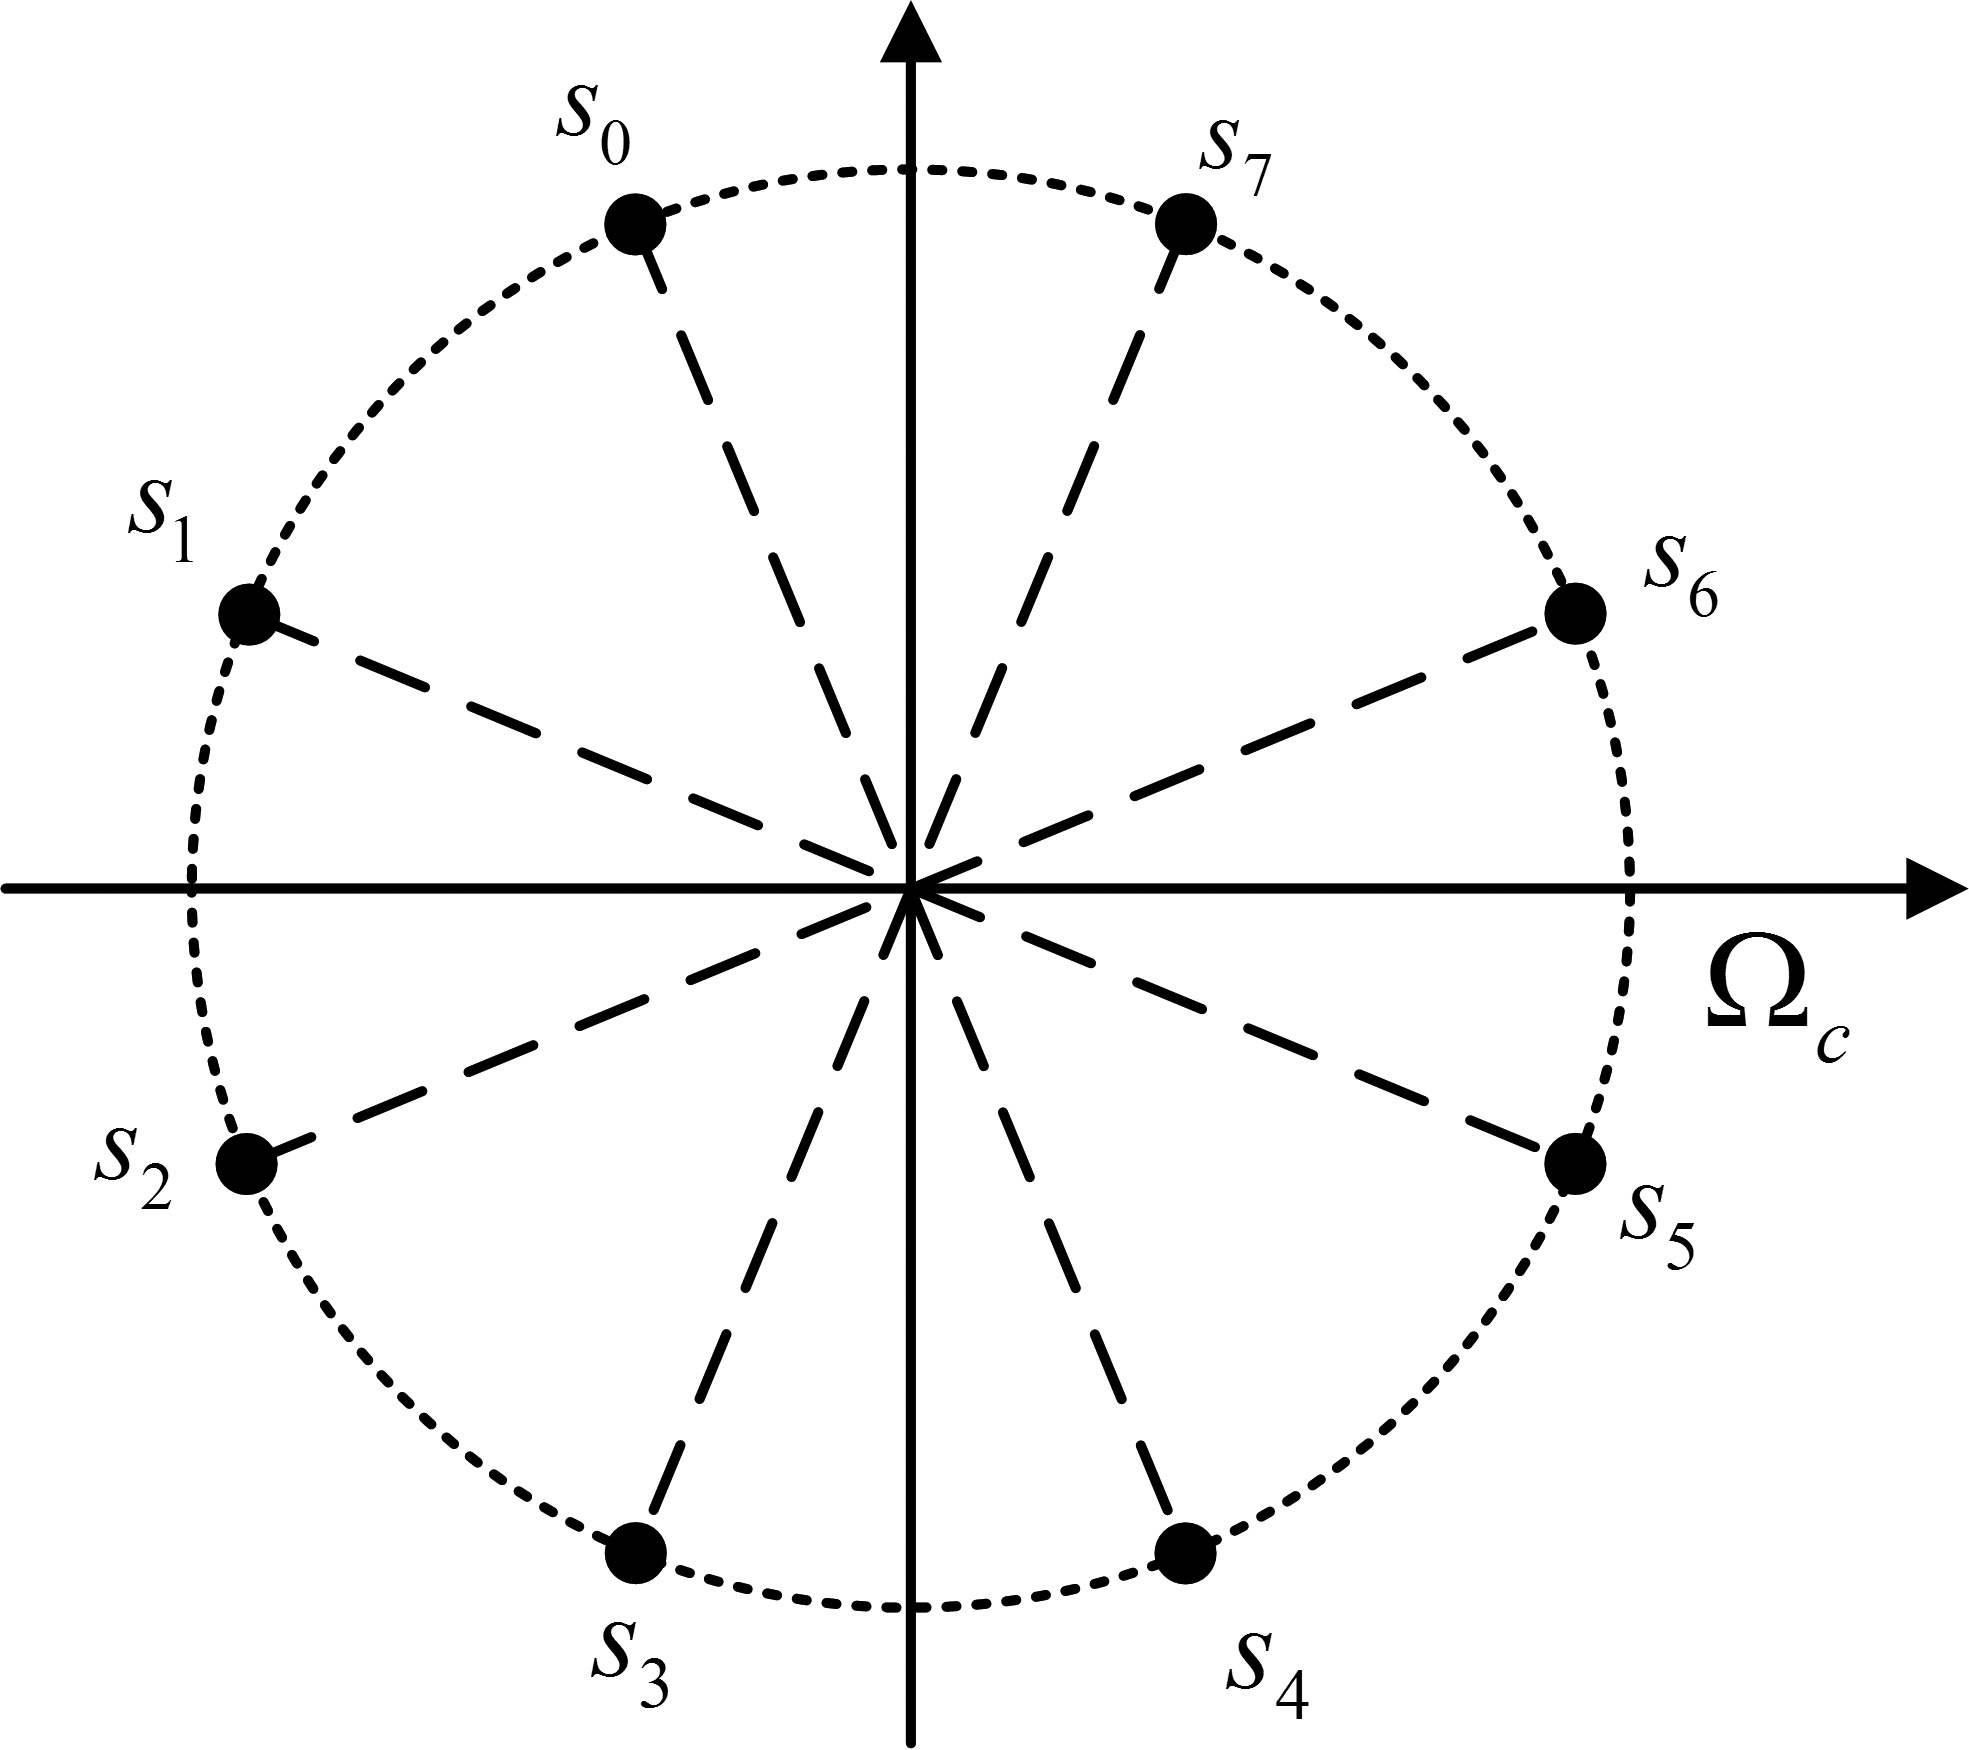
\includegraphics[width=0.4\textwidth]{fig8_example.jpg}
          %\caption{极点分布图}
          %\vspace{-0.8cm}
          %\label{}
      \end{figure}

      可见,$s_{0},s_{1},s_{2},s_{3}$在s平面左边,$s_{4},s_{5},s_{6},s_{7}$在s平面
      右边,$s_{k}$分布在半径为$\Omega_{c}$的圆上,且关于原点对称。
\end{frame}
%%%%%%%%%%%%%%%%%%%%%%%%%%%%%%%%%%%%%%%%%%%%%%%%%%%%%%%%%%%%%%%%%%%%%%%%%%%%%%%%%%%%%%%%%%%%%%


%%%%%%%%%%%%%%%%%%%%%%%%%%%%%%%%%%%%%%%%%%%%%%%%%%%%%%%%%%%%%%%%%%%%%%%%%%%%%%%%%%%%%%%%%%%%%%
\begin{frame}\frametitle{}%[allowframebreaks]
\begin{enumerate}
\item [(3)]
      由s左半平面N个极点
      $$s_{k}=\Omega_{c}\cdot e^{j\pi[\frac{1}{2}+\frac{2k+1)}{2N}]}\quad\quad\quad k=0,1,...,(N-1)$$
      构造出$H_{a}(s)$。
      $$
        \left\{ \begin{aligned}
            H_{a}(s) &= \frac{\Omega_{c}^{N}}{\prod^{N-1}_{k=0}(s-s_{k})}\quad\quad k=0,1,...,(N-1)\\
          \mbox{式中:}  s_{k}    &= \Omega_{c}\cdot e^{j\pi[\frac{1}{2}+\frac{2k+1}{2N}]}\\
        \end{aligned} \right.
      $$
%       $$\mbox{令:}\quad s_{k} =\Omega_{c}\cdot e^{j\pi\left[\frac{1}{2}+\frac{2k+1}{2N}\right]}  \quad\quad k=0,1,...,(N-1)$$
%       $$\mbox{则:}\quad H_{a}(s) = \frac{\Omega_{c}^{N}}{\prod^{N-1}_{k=0}(s-s_{k})}\quad\quad\quad\quad\quad\quad\quad\quad\quad$$
%      $$
%        \left\{ \begin{aligned}
%            \mbox{令:}\quad s_{k} &=\Omega_{c}\cdot e^{j\pi\left[\frac{1}{2}+\frac{2k+1}{2N}\right]}  \quad\quad k=0,1,...,(N-1) \\
%            H_{a}(s) &= \frac{\Omega_{c}^{N}}{\prod^{N-1}_{k=0}(s-s_{k})}
%        \end{aligned} \right.
%      $$
\end{enumerate}
\end{frame}
%%%%%%%%%%%%%%%%%%%%%%%%%%%%%%%%%%%%%%%%%%%%%%%%%%%%%%%%%%%%%%%%%%%%%%%%%%%%%%%%%%%%%%%%%%%%%%


%%%%%%%%%%%%%%%%%%%%%%%%%%%%%%%%%%%%%%%%%%%%%%%%%%%%%%%%%%%%%%%%%%%%%%%%%%%%%%%%%%%%%%%%%%%%%%
\begin{frame}\frametitle{}%[allowframebreaks]
\textbf{\heiti 二、设计过程}

\begin{enumerate}
\item  由$(\Omega_{p},\alpha_{p})$,$(\Omega_{s},\alpha_{s})$得到:
      $$|H_{a}(j\Omega)|^{2}= \frac{1}{1+(\frac{\Omega}{\Omega_{c}})^{2N}}$$
      即求解$N,\Omega_{c}$
  \item   由
  $|H_a(j\Omega)|^{2}\longrightarrow H_{a}(s)$
      $$
        \left\{ \begin{aligned}
            \mbox{令:}\quad s_{k} &=\Omega_{c}\cdot e^{j\pi\left[\frac{1}{2}+\frac{2k+1}{2N}\right]}  \quad\quad k=0,1,...,(N-1) \\
            H_{a}(s) &= \frac{\Omega_{c}^{N}}{\prod^{N-1}_{k=0}(s-s_{k})}
        \end{aligned} \right.
      $$
\end{enumerate}
\end{frame}
%%%%%%%%%%%%%%%%%%%%%%%%%%%%%%%%%%%%%%%%%%%%%%%%%%%%%%%%%%%%%%%%%%%%%%%%%%%%%%%%%%%%%%%%%%%%%%


%%%%%%%%%%%%%%%%%%%%%%%%%%%%%%%%%%%%%%%%%%%%%%%%%%%%%%%%%%%%%%%%%%%%%%%%%%%%%%%%%%%%%%%%%%%%%%
\begin{frame}\frametitle{例题}%[allowframebreaks]
\begin{example}
已知,$f_p=5kHz$, $\alpha_p=3dB$ ,$f_s=10kHz$, $\alpha_s=30db$,按照以上技术指标设计巴特沃斯低通滤波器,求阶数N。
\end{example}
\begin{answer}
写成标准形式:
%\end{answer}
$$
\left\{
\begin{aligned}
\Omega_{p}  &=2\pi f_p= 10\pi \times 10^{3} \quad\quad rad/s\\
\alpha_{p}  &= 3 dB\quad\quad\quad\quad\quad\quad\quad\\
\end{aligned}
\right.
$$
$$
\left\{
\begin{aligned}
\Omega_{s}  &=2\pi f_s= 20\pi \times 10^{3} \quad\quad rad/s\\
\alpha_{s}  &= 30 dB\quad\quad\quad\quad\quad\quad\quad\\
\end{aligned}
\right.
$$

\end{answer}
%        \begin{flushleft}
%        $$\mbox{代入}\quad\quad\quad\quad
%        1+(\frac{\Omega}{\Omega_{c}})^{2N}=10^{\frac{\alpha(\Omega)}{10}}
%        \quad\quad\quad\quad\quad\quad\quad\quad\quad\quad$$
%        \end{flushleft}
%\end{answer}
%\begin{dablock}
%\end{dablock}
\end{frame}
%%%%%%%%%%%%%%%%%%%%%%%%%%%%%%%%%%%%%%%%%%%%%%%%%%%%%%%%%%%%%%%%%%%%%%%%%%%%%%%%%%%%%%%%%%%%%%


%%%%%%%%%%%%%%%%%%%%%%%%%%%%%%%%%%%%%%%%%%%%%%%%%%%%%%%%%%%%%%%%%%%%%%%%%%%%%%%%%%%%%%%%%%%%%%
\begin{frame}[shrink]\frametitle{}%[allowframebreaks]
\begin{dablock}
        \begin{flushleft}
        $$\mbox{代入}\quad\quad\quad\quad
        1+(\frac{\Omega}{\Omega_{c}})^{2N}=10^{\frac{\alpha(\Omega)}{10}}
        \quad\quad\quad\quad\quad\quad\quad\quad\quad\quad$$
        \end{flushleft}
        可得:
        $$
        \left\{ \begin{aligned}
            1+(\frac{\Omega_{p}}{\Omega_{c}})^{2N} &= 10^{\frac{3}{10}}\\
            1+(\frac{\Omega_{s}}{\Omega_{c}})^{2N} &= 10^{3}\\
        \end{aligned} \right.
        $$
        联立求解得:
        $$(\frac{\Omega_{p}}{\Omega_{s}})^{2N} = \frac{10^{\frac{3}{10}}-1}{10^{3}-1}$$
        $$\mbox{$N=4.98$}$$
        但N为阶数,必须为整数。
%        $$
%        \left\{ \begin{aligned}
%            N          &= 5\\
%            \Omega_{c} &= 10^{4}\pi\quad rad/s\\
%        \end{aligned} \right.
%        $$
\end{dablock}
\end{frame}
%%%%%%%%%%%%%%%%%%%%%%%%%%%%%%%%%%%%%%%%%%%%%%%%%%%%%%%%%%%%%%%%%%%%%%%%%%%%%%%%%%%%%%%%%%%%%%
%
%
%%%%%%%%%%%%%%%%%%%%%%%%%%%%%%%%%%%%%%%%%%%%%%%%%%%%%%%%%%%%%%%%%%%%%%%%%%%%%%%%%%%%%%%%%%%%%%
\begin{frame}[shrink]\frametitle{}%[allowframebreaks]
\begin{dablock}
因为N必须为整数,有
$$
\left\{ \begin{aligned}
N          &= 5\\
\Omega_{c} &= 10^{4}\pi\quad rad/s\\
\end{aligned} \right.
$$
计算$s_k$:
$$s_{k}=\Omega_{c}\cdot e^{j\pi[\frac{1}{2}+\frac{2k+1)}{2N}]} \qquad (k=0,1,2,3,4)$$
$$\therefore\quad\quad H(s)= \frac{\Omega^{5}_{c}}{\prod^4_{0}(s-s_k)}\qquad\qquad\qquad\qquad$$

%$$H(s)= \frac{\pi^{5}\cdot 10^{20}}{(s+10^4\pi)[s^2+0.618\pi\times10^4s+(\pi\times10^4)^2]}\\
%\frac{1}{
%[s^2+1.618\pi\times10^4s+(\pi\times10^4)^2]}$$
\begin{equation*}
\begin{split}
  H(s) &=     \frac{\pi^{5}\cdot 10^{20}}{(s+10^4\pi)[s^2+0.618\pi\times10^4s+(\pi\times10^4)^2]}\cdot \\
       &\quad \quad\quad\frac{1}{[s^2+1.618\pi\times10^4s+(\pi\times10^4)^2]}
\end{split}
\end{equation*}
\end{dablock}
\end{frame}
%%%%%%%%%%%%%%%%%%%%%%%%%%%%%%%%%%%%%%%%%%%%%%%%%%%%%%%%%%%%%%%%%%%%%%%%%%%%%%%%%%%%%%%%%%%%%%
%
%
%%%%%%%%%%%%%%%%%%%%%%%%%%%%%%%%%%%%%%%%%%%%%%%%%%%%%%%%%%%%%%%%%%%%%%%%%%%%%%%%%%%%%%%%%%%%%%
\begin{frame}\frametitle{三、查表法}%[allowframebreaks]
%三、查表法

    在最平响应Butterworth滤波器的设计中,我们总是由
      $$
        \left\{
        \begin{aligned}
        (\Omega_{p},\alpha_{p})\\
        (\Omega_{s},\alpha_{s})\\
        \end{aligned}
        \right.
      $$
      得到$N,\Omega_{c}$,计算过程很复杂。

      但我们发现由:
       $$\left(\frac{\Omega_{p}}{\Omega_{s}}\right)^{2N} = \frac{10^{\frac{\alpha_{p}}{10}-1}}{10^{\frac{\alpha_{s}}{10}-1}} \Longrightarrow N$$
       \par 的过程与$\Omega_c$无关,\textbf{即滤波器的阶数N与$\Omega_c$无关}。

       \textbf{考虑:}将计算过程标准化。
\end{frame}
%%%%%%%%%%%%%%%%%%%%%%%%%%%%%%%%%%%%%%%%%%%%%%%%%%%%%%%%%%%%%%%%%%%%%%%%%%%%%%%%%%%%%%%%%%%%%%
%
%
%%%%%%%%%%%%%%%%%%%%%%%%%%%%%%%%%%%%%%%%%%%%%%%%%%%%%%%%%%%%%%%%%%%%%%%%%%%%%%%%%%%%%%%%%%%%%%
\begin{frame}[allowframebreaks]\frametitle{}%[allowframebreaks]
\begin{enumerate}
       \item  [1]原理

         令 $p=\frac{s}{\Omega_c}$  (归一化广义频率)
         则:
         $$s_k= \Omega_c\cdot e^{j\pi[\frac{1}{2}+\frac{2k+1}{2N}]}\quad  \Longrightarrow\quad
         p_k= \dfrac{s_k}{\Omega_c} = e^{j\pi[\frac{1}{2}+\frac{2k+1}{2N}]}\mbox{\quad 与$\Omega_c$无关}
         $$
         而
         $$H_{a}(s) = \frac{\Omega_{c}^{N}}{\prod^{N-1}_{k=0}(s-s_{k})}
         = \frac{1}{\prod^{N-1}_{k=0}(\frac{s}{\Omega_{c}}-\frac{s_{k}}
         {\Omega_{c}})}
         = \frac{1}{\prod^{N-1}_{k=0}(p-p_{k})}$$
         此处,$p=s/\Omega_c$,$p_k=s_k/\Omega_c$
\newpage
         令:
         $$H_{a}(p)= \frac{1}{\prod^{N-1}_{k=0}(p-p_{k})}$$
         \begin{enumerate}
           \item $H_{a}(p)$仅与N有关,与$\Omega_c$无关;
           \item $H_a(p)$称为归一化传输函数。
         \end{enumerate}

       \item  [2]查表法设计步骤
         \begin{enumerate}
           \item 根据指定技术指标$(\Omega_p,\alpha_p),(\Omega_s,\alpha_s)$,确定$N,\Omega_c$。
           \item 由N查表得到归一化传输函数$H_a(p)$。
           \item 去归一化。
               $$H_a(s) = H_a(p)|_{p=s/\Omega_c}$$
         \end{enumerate}

       \end{enumerate}
\end{frame}
%%%%%%%%%%%%%%%%%%%%%%%%%%%%%%%%%%%%%%%%%%%%%%%%%%%%%%%%%%%%%%%%%%%%%%%%%%%%%%%%%%%%%%%%%%%%%%
\section{6.3 IIR-DF的设计—脉冲响应不变法}

\subsection{6.3.1 IIR-DF设计的基本概念}
\subsubsection*{基本概念}
%%%%%%%%%%%%%%%%%%%%%%%%%%%%%%%%%%%%%%%%%%%%%%%%%%%%%%%%%%%%%%%%%%%%%%%%%%%%%%%%%%%%%%%%%%%%%%
\begin{frame}[shrink]\frametitle{}%[allowframebreaks]
{\heiti 一、基本概念}
\begin{enumerate}
  \item [(1)]
    技术要求 $H(e^{j\omega})$,即:    $\quad\quad(\omega_p,\alpha_p),(\omega_s,\alpha_s)$
    \begin{figure}[h]
    \centering
    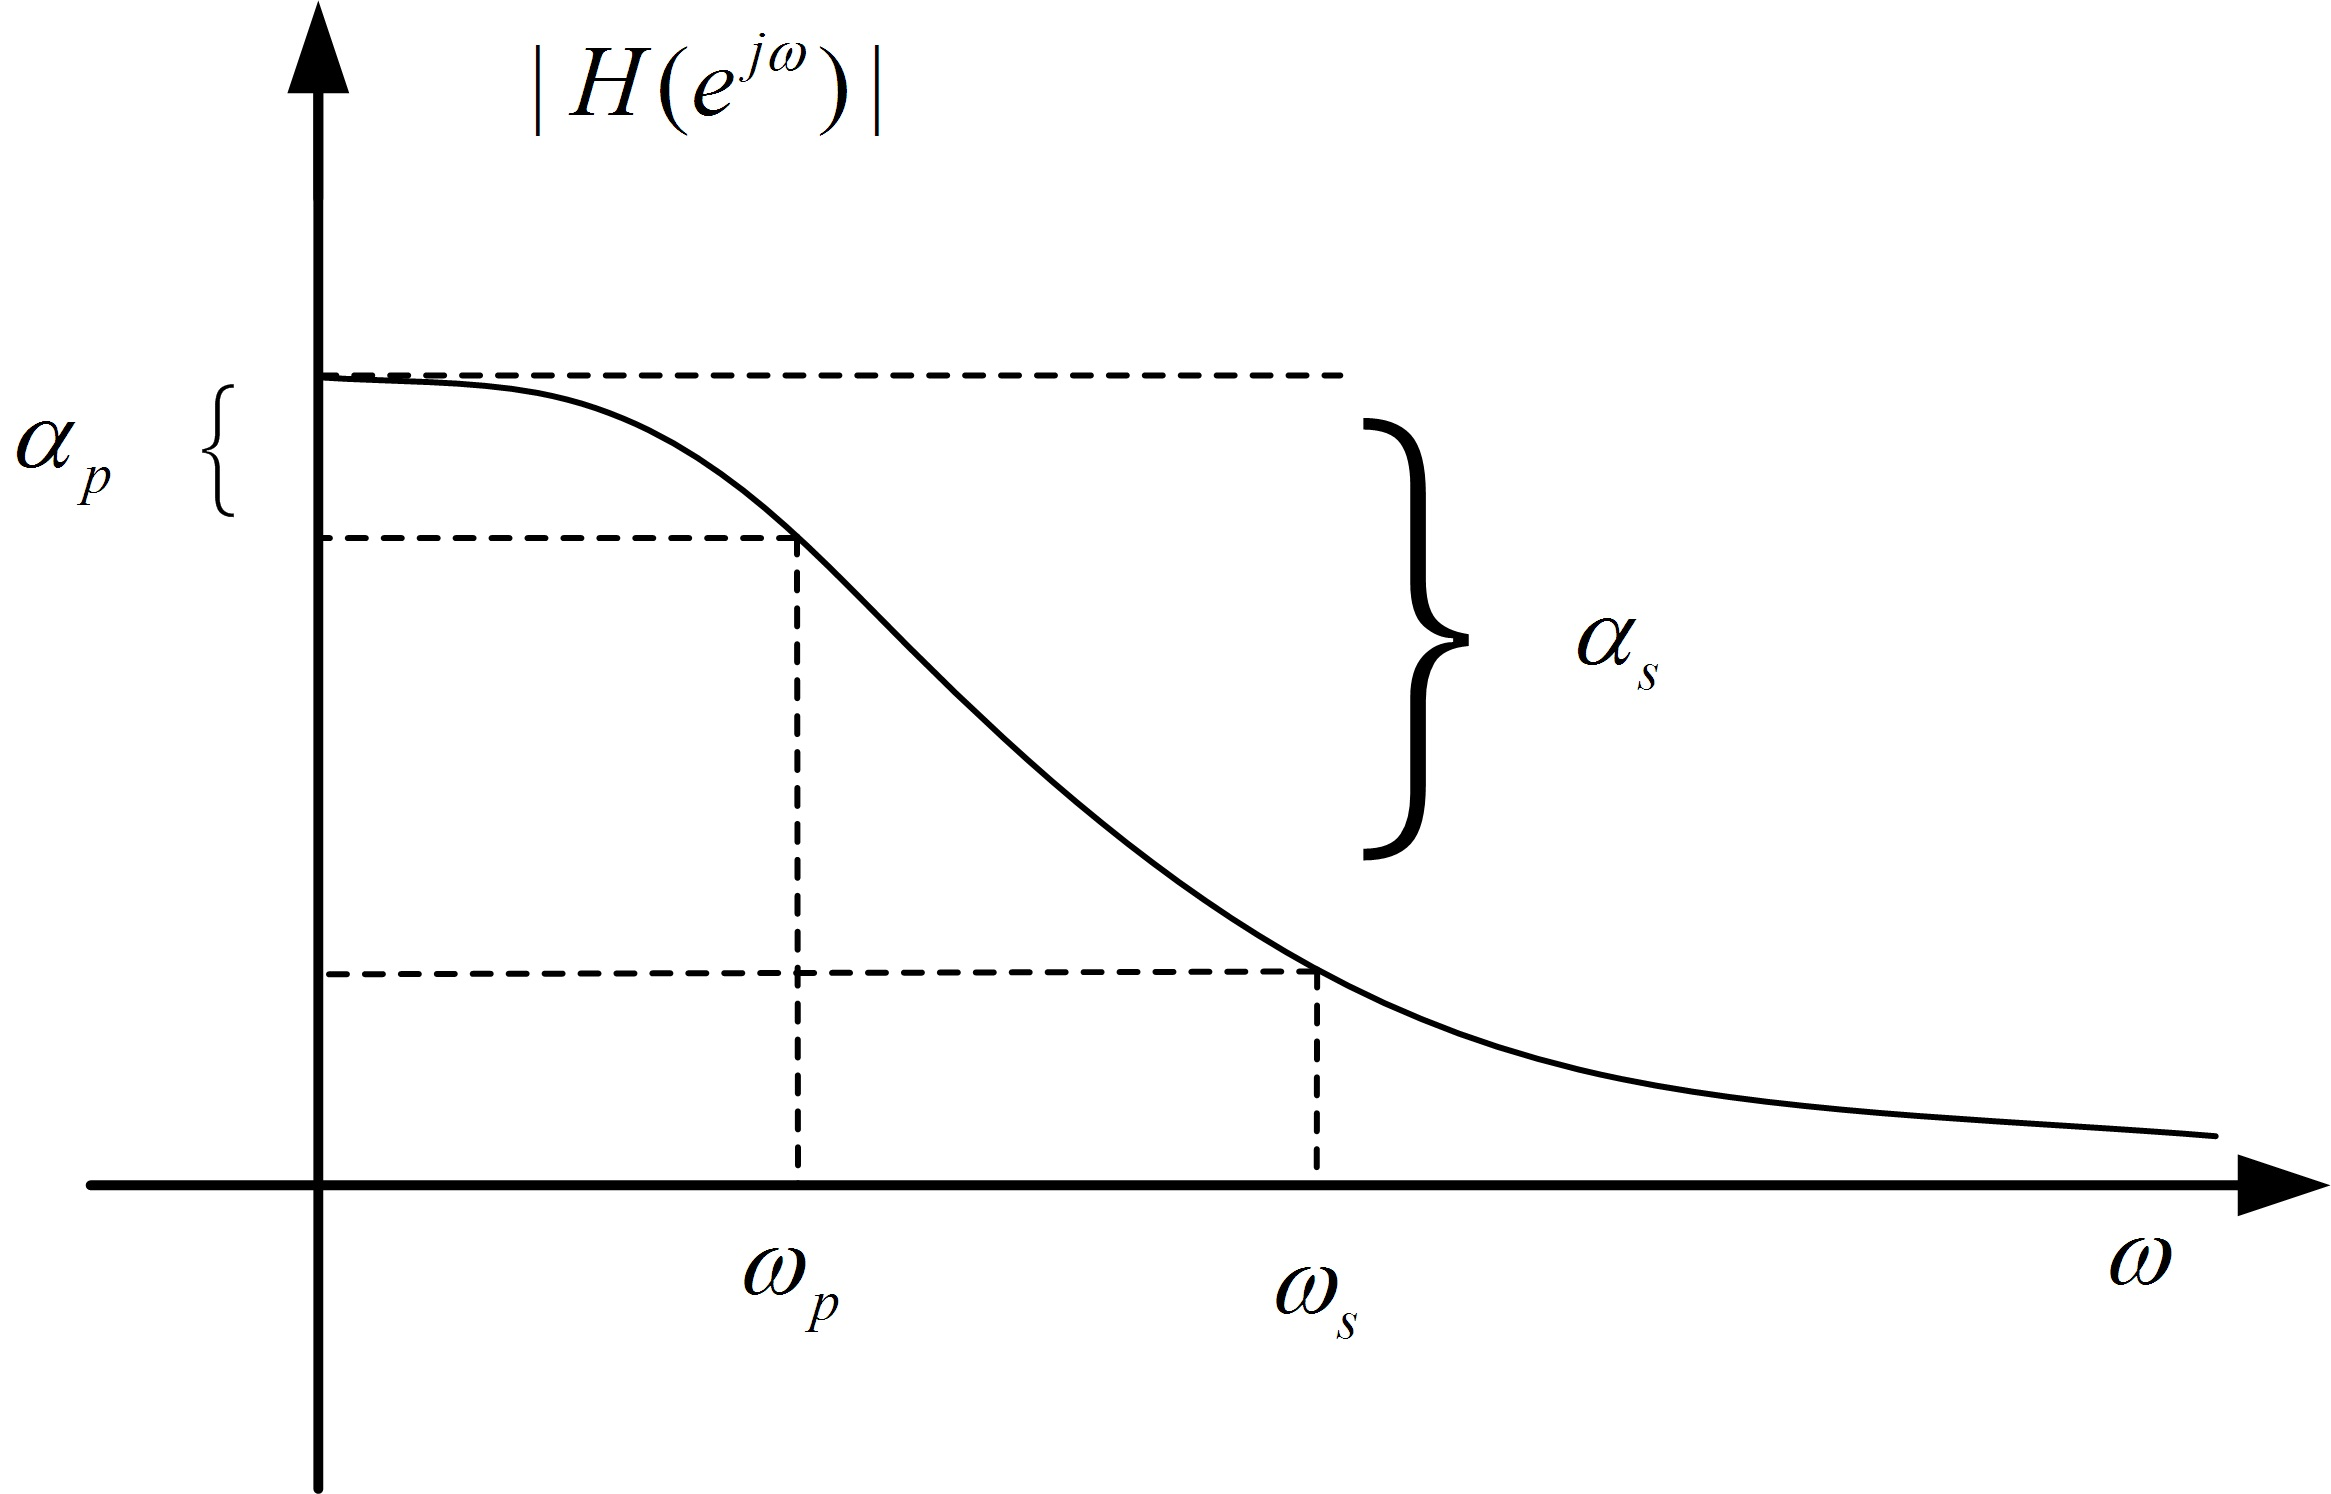
\includegraphics[width=0.5\textwidth]{fig9_lpdfjszb.jpg}
    \caption{数字滤波器的幅频特性指标示意图}
    %\label{}
    %\vspace{-0.8cm}
    \end{figure}
  \item [(2)] 衰减函数
  $$\alpha(\omega)=-20lg\frac{|H(e^{j\omega})|}{|H(e^{j0})}= 10lg\frac{1}{|H(e^{j\omega})|^2}$$
\end{enumerate}
\end{frame}
%%%%%%%%%%%%%%%%%%%%%%%%%%%%%%%%%%%%%%%%%%%%%%%%%%%%%%%%%%%%%%%%%%%%%%%%%%%%%%%%%%%%%%%%%%%%%%
%
%
%%%%%%%%%%%%%%%%%%%%%%%%%%%%%%%%%%%%%%%%%%%%%%%%%%%%%%%%%%%%%%%%%%%%%%%%%%%%%%%%%%%%%%%%%%%%%%
\begin{frame}\frametitle{}%[allowframebreaks]
\begin{enumerate}
\item [(3)] $H(e^{j\omega})$与$H_a(j\Omega)$的不同之处在于:
  \begin{enumerate}
    \item $H(e^{j\omega})$是$\omega$的周期函数,且周期为$2\pi$。
    \item $H(e^{j\omega})$在$\pi$附近称为高频,在$0(2\pi)$附近称为低频。
  \end{enumerate}

  \begin{figure}[h]
    \centering
    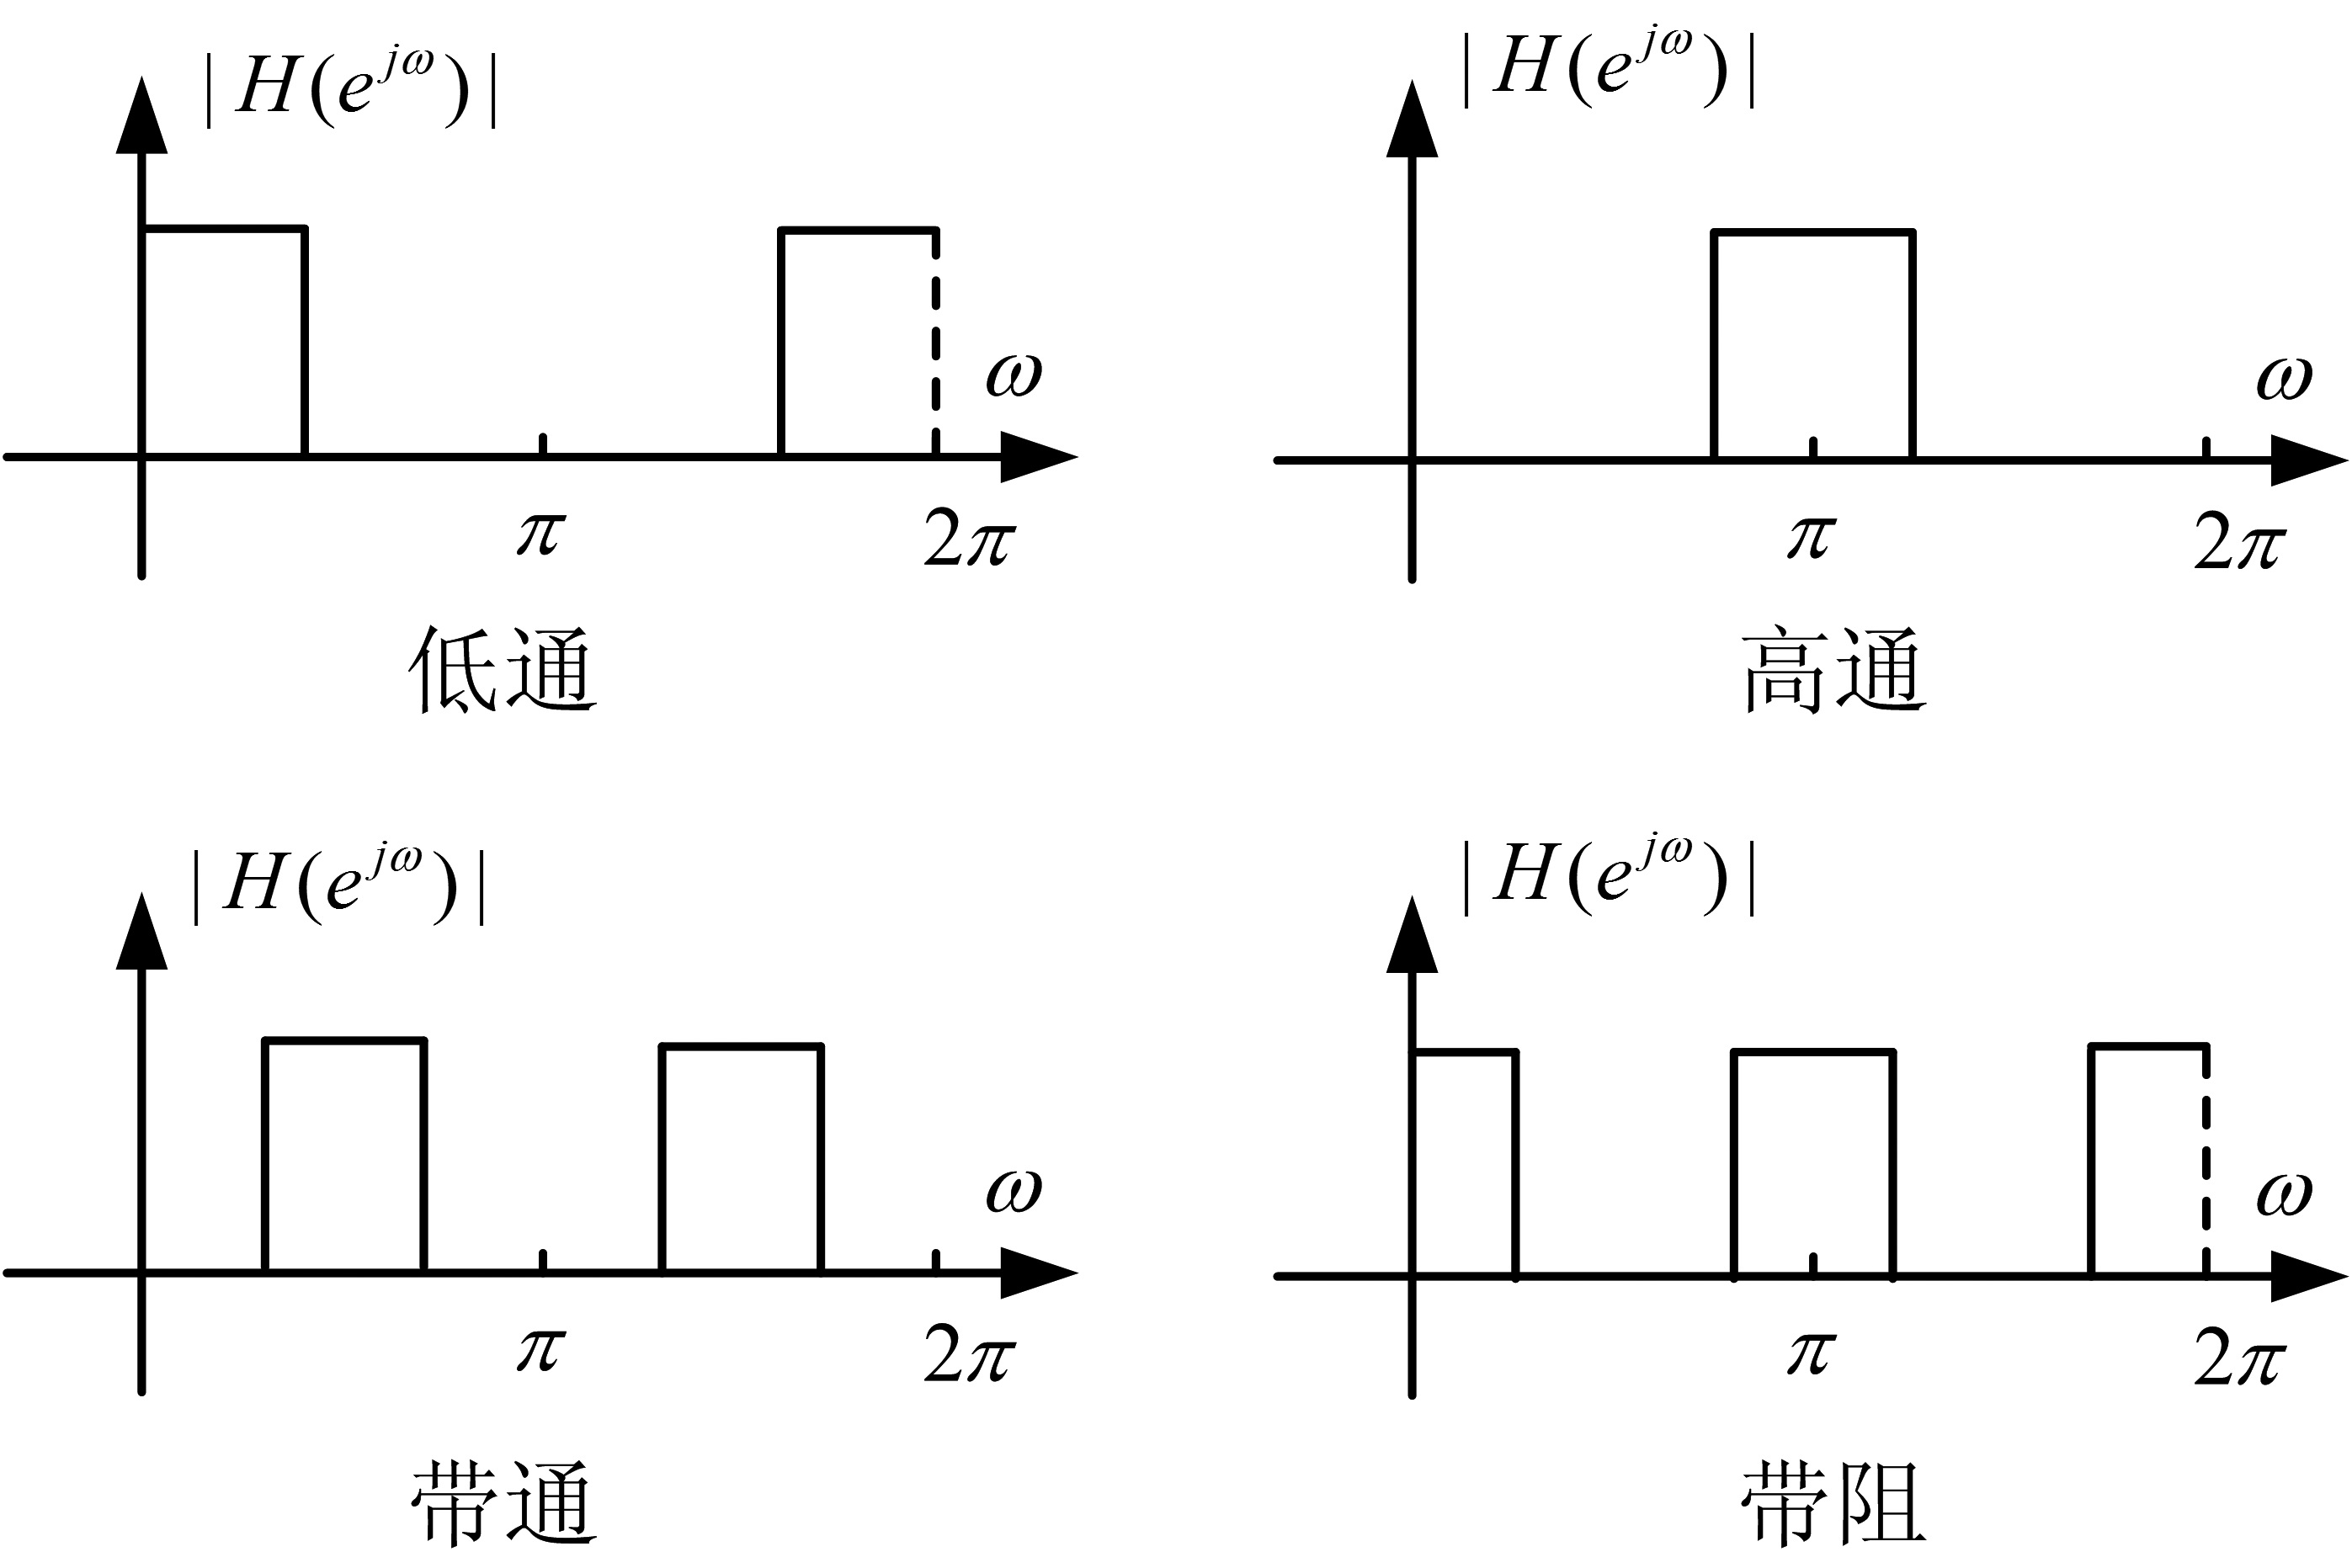
\includegraphics[width=0.65\textwidth]{fig10_shuzilvboqi.jpg}
    \caption{各种理想数字滤波器的幅频特性}
    %\label{}
    %\vspace{-0.8cm}
   \end{figure}
   \end{enumerate}
\end{frame}
%%%%%%%%%%%%%%%%%%%%%%%%%%%%%%%%%%%%%%%%%%%%%%%%%%%%%%%%%%%%%%%%%%%%%%%%%%%%%%%%%%%%%%%%%%%%%%
\subsubsection*{从AF设计DF的基本思想}
%%%%%%%%%%%%%%%%%%%%%%%%%%%%%%%%%%%%%%%%%%%%%%%%%%%%%%%%%%%%%%%%%%%%%%%%%%%%%%%%%%%%%%%%%%%%%%
\begin{frame}[shrink]\frametitle{}%[allowframebreaks]
{\heiti 二、从AF设计DF的基本思想}
\begin{enumerate}
  \item [1] 将数字滤波器的技术指标转化为模拟滤波器的技术指标。 \newline
  \item [2] 设计模拟滤波器,得到其系统函数$H_a(s)$。 \newline
  \item [3] $H_a(s)\quad\underrightarrow{\quad\mbox{映射}\quad}\quad H(z)$\quad 映射方法:\newline
      \begin{enumerate}
        \item [(1)]脉冲响应不变法 \newline
        \item [(2)]双线性映射法   \newline
      \end{enumerate}
\end{enumerate}
%为此,映射关系要满足以下两条:\par
%\begin{enumerate}
%    \item 映射前后,系统的因果稳定性不变。
%
%    $\Longleftrightarrow \mbox{s左半平面上任何一点,映射到z平面单位圆内部。}$
%
%    \item 数字滤波器的频率响应函数$H(e^{j\omega})$能模仿模拟滤波器的频率响应函数$H_a(j\Omega)$。
%
%    $\Longleftrightarrow \mbox{s平面虚轴上的点映射到z平面单位圆上。}$
%
%  \end{enumerate}
\end{frame}
%%%%%%%%%%%%%%%%%%%%%%%%%%%%%%%%%%%%%%%%%%%%%%%%%%%%%%%%%%%%%%%%%%%%%%%%%%%%%%%%%%%%%%%%%%%%%%
%
%
%%%%%%%%%%%%%%%%%%%%%%%%%%%%%%%%%%%%%%%%%%%%%%%%%%%%%%%%%%%%%%%%%%%%%%%%%%%%%%%%%%%%%%%%%%%%%%
\begin{frame}\frametitle{\quad\quad\quad\quad\quad
从AF设计DF的基本思想的示意图
}%[allowframebreaks]
%从AF设计DF的基本思想的示意图
  \begin{figure}[h]
    \centering
    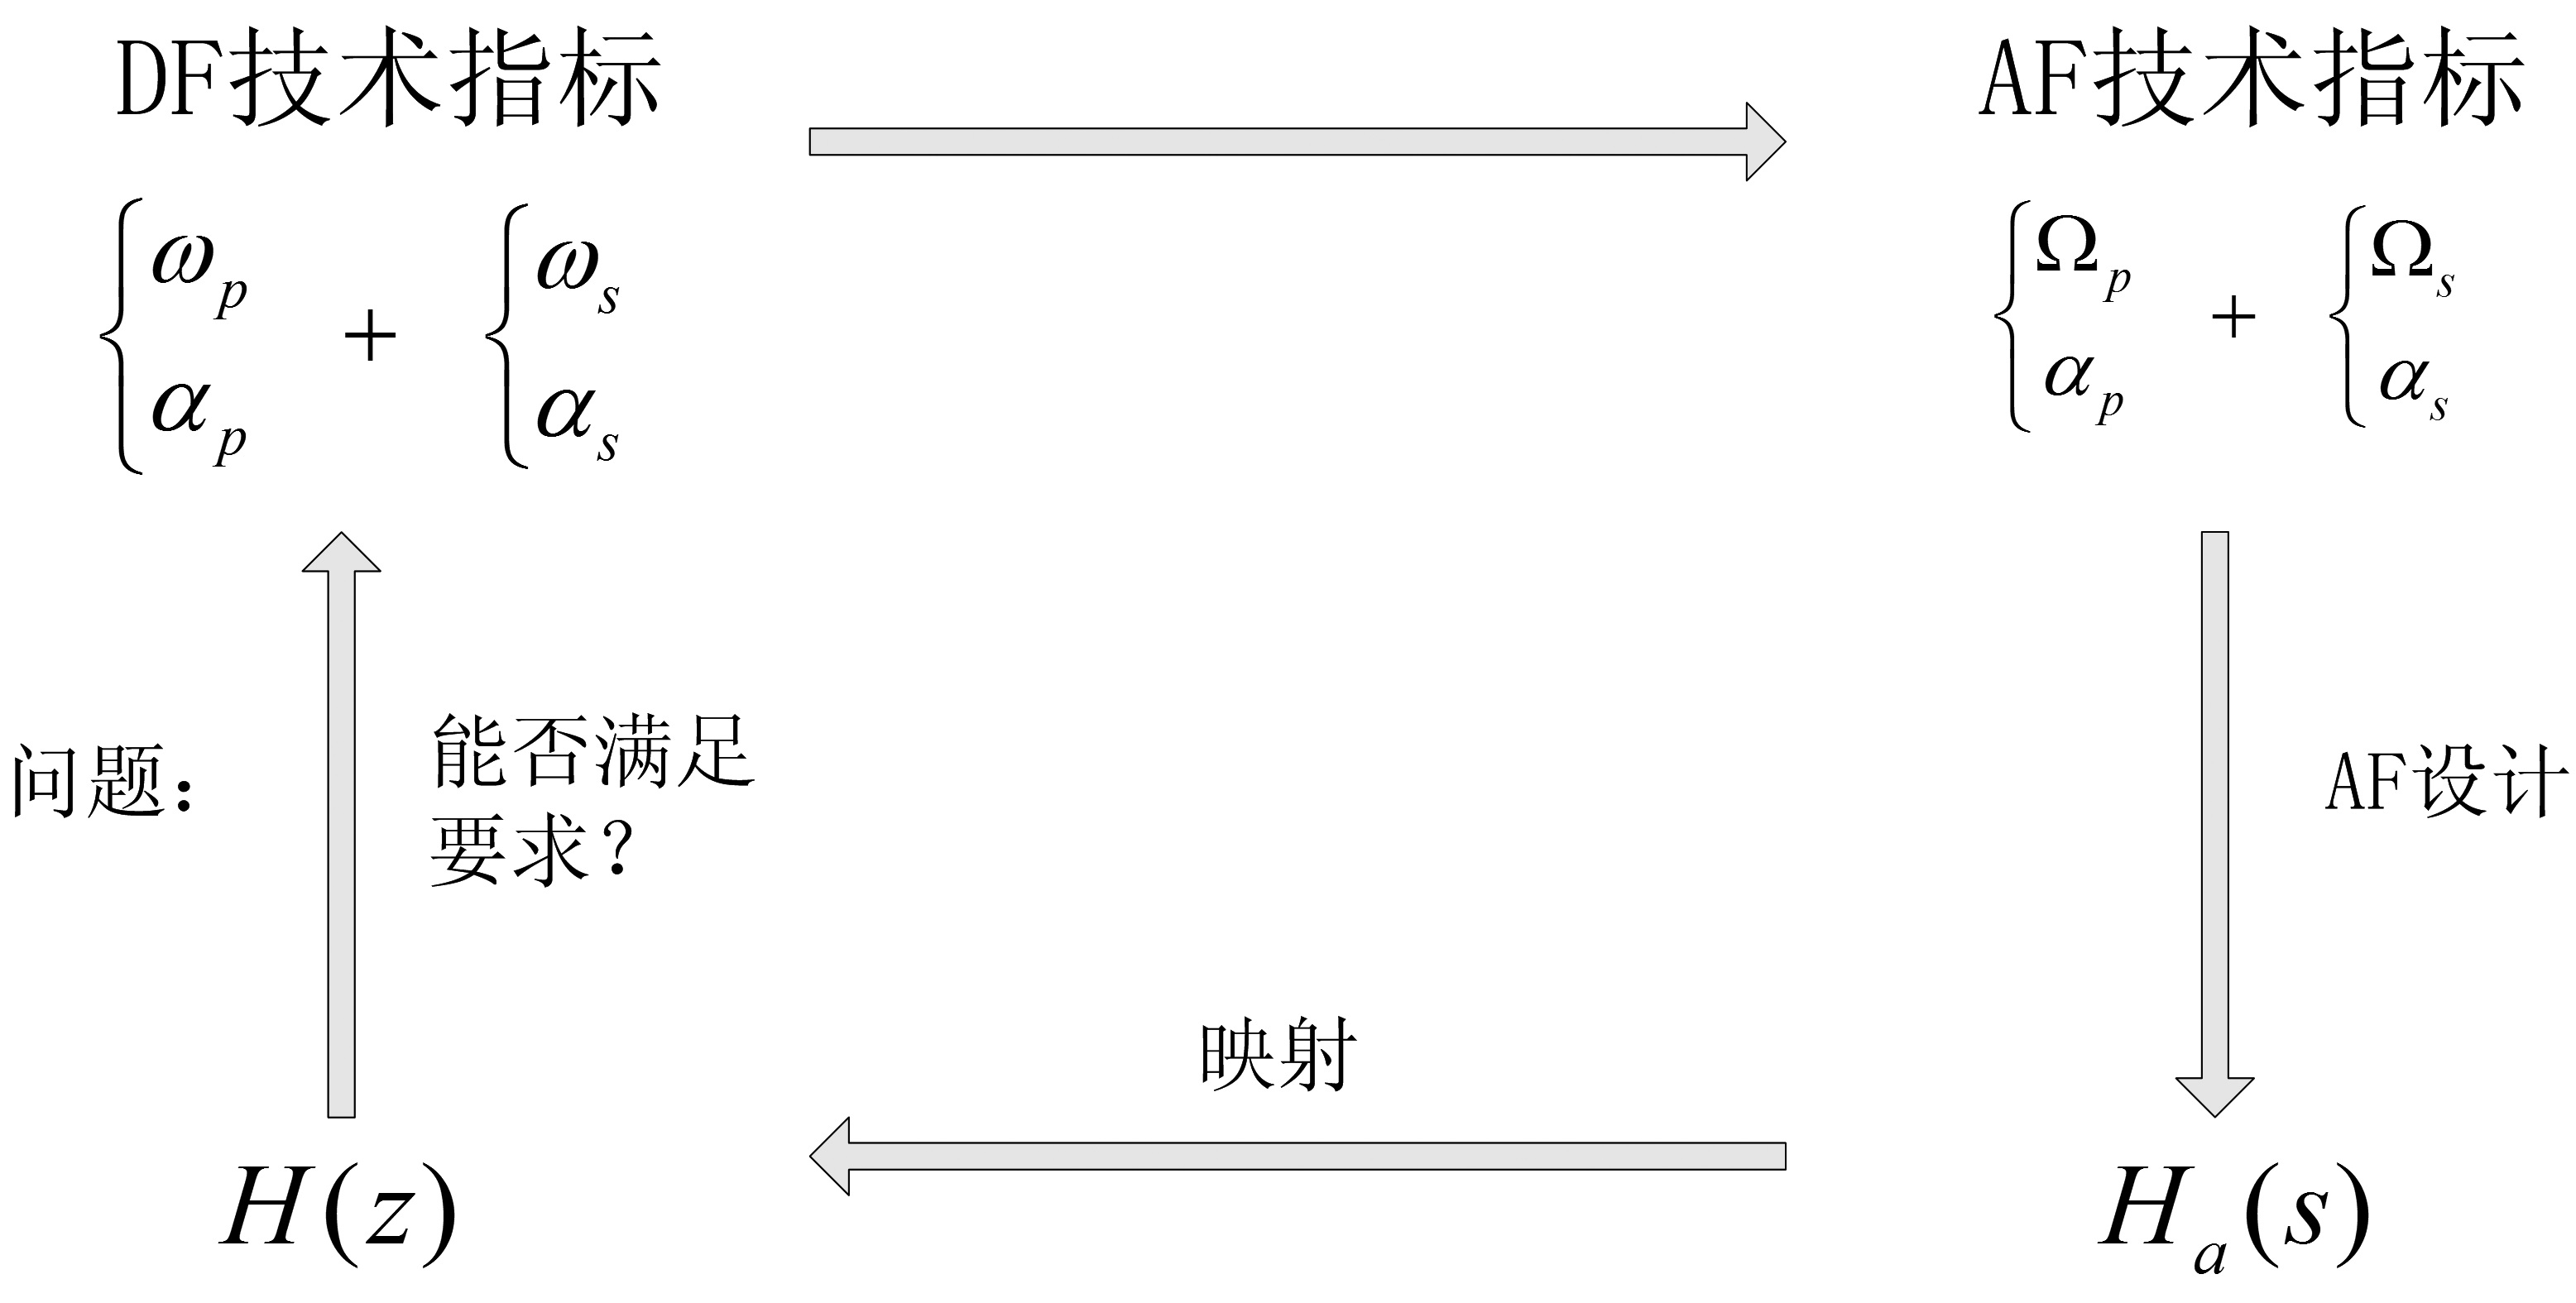
\includegraphics[width=0.85\textwidth]{fig11_afdfshejisilu.jpg}
    %\caption{从AF设计DF的基本思想的示意图}   %\label{}
  \end{figure}
  %\pause
  \begin{dablock}
      关键在于:找到一种映射关系,使得$H(z)$满足数字滤波器的技术指标。
  \end{dablock}
\end{frame}
%



\begin{frame}[shrink]\frametitle{映射关系需要满足的条件}%[allowframebreaks]
  \begin{dablock}
      如何使得$H(z)$满足数字滤波器的技术指标。\par
      为此,映射关系要满足以下两条:\par
  \end{dablock}

\begin{enumerate}
    \item [1] 映射前后,系统的因果稳定性不变。
    \newline
    $\Longleftrightarrow \mbox{s左半平面上任何一点,映射到z平面单位圆内部。}$
    \newline
    \item [2] 数字滤波器的频率响应函数$H(e^{j\omega})$能模仿模拟滤波器的频率响应函数$H_a(j\Omega)$。
    \newline
    $\Longleftrightarrow \mbox{s平面虚轴上的点映射到z平面单位圆上。}$
    \newline
  \end{enumerate}
\end{frame}
%%%%%%%%%%%%%%%%%%%%%%%%%%%%%%%%%%%%%%%%%%%%%%%%%%%%%%%%%%%%%%%%%%%%%%%%%%%%%%%%%%%%%%%%%%%%%%
%
%

%%%%%%%%%%%%%%%%%%%%%%%%%%%%%%%%%%%%%%%%%%%%%%%%%%%%%%%%%%%%%%%%%%%%%%%%%%%%%%%%%%%%%%%%%%%%%


\subsection{6.3.2 脉冲响应不变法}
%\subsubsection{原理}
%%%%%%%%%%%%%%%%%%%%%%%%%%%%%%%%%%%%%%%%%%%%%%%%%%%%%%%%%%%%%%%%%%%%%%%%%%%%%%%%%%%%%%%%%%%%%%
\begin{frame}[shrink]\frametitle{问题:已知$H_a(s)$,求$\quad H(z)$}%[allowframebreaks]
%\textbf{问题:已知$H_a(s)$,求$\quad H(z)$}

一、原理
  $$\mbox{设}\quad\quad\quad
  h_a(t) \longleftrightarrow H_a(s)\quad\quad\quad
   \mbox{且}\quad\quad h(n) \longleftrightarrow H(z)\quad$$
  $$\mbox{令}\quad\quad\quad h(n)=h_a(t)|_{t=nT}\quad\quad\quad
  \quad\quad\mbox{(脉冲响应不变)}$$
  二、推导
$$\mbox{思路:}\quad\quad H_a(s)\longrightarrow h_a(t) \longrightarrow h(n) \longrightarrow H(z)$$
  \begin{figure}[h]
    \centering
    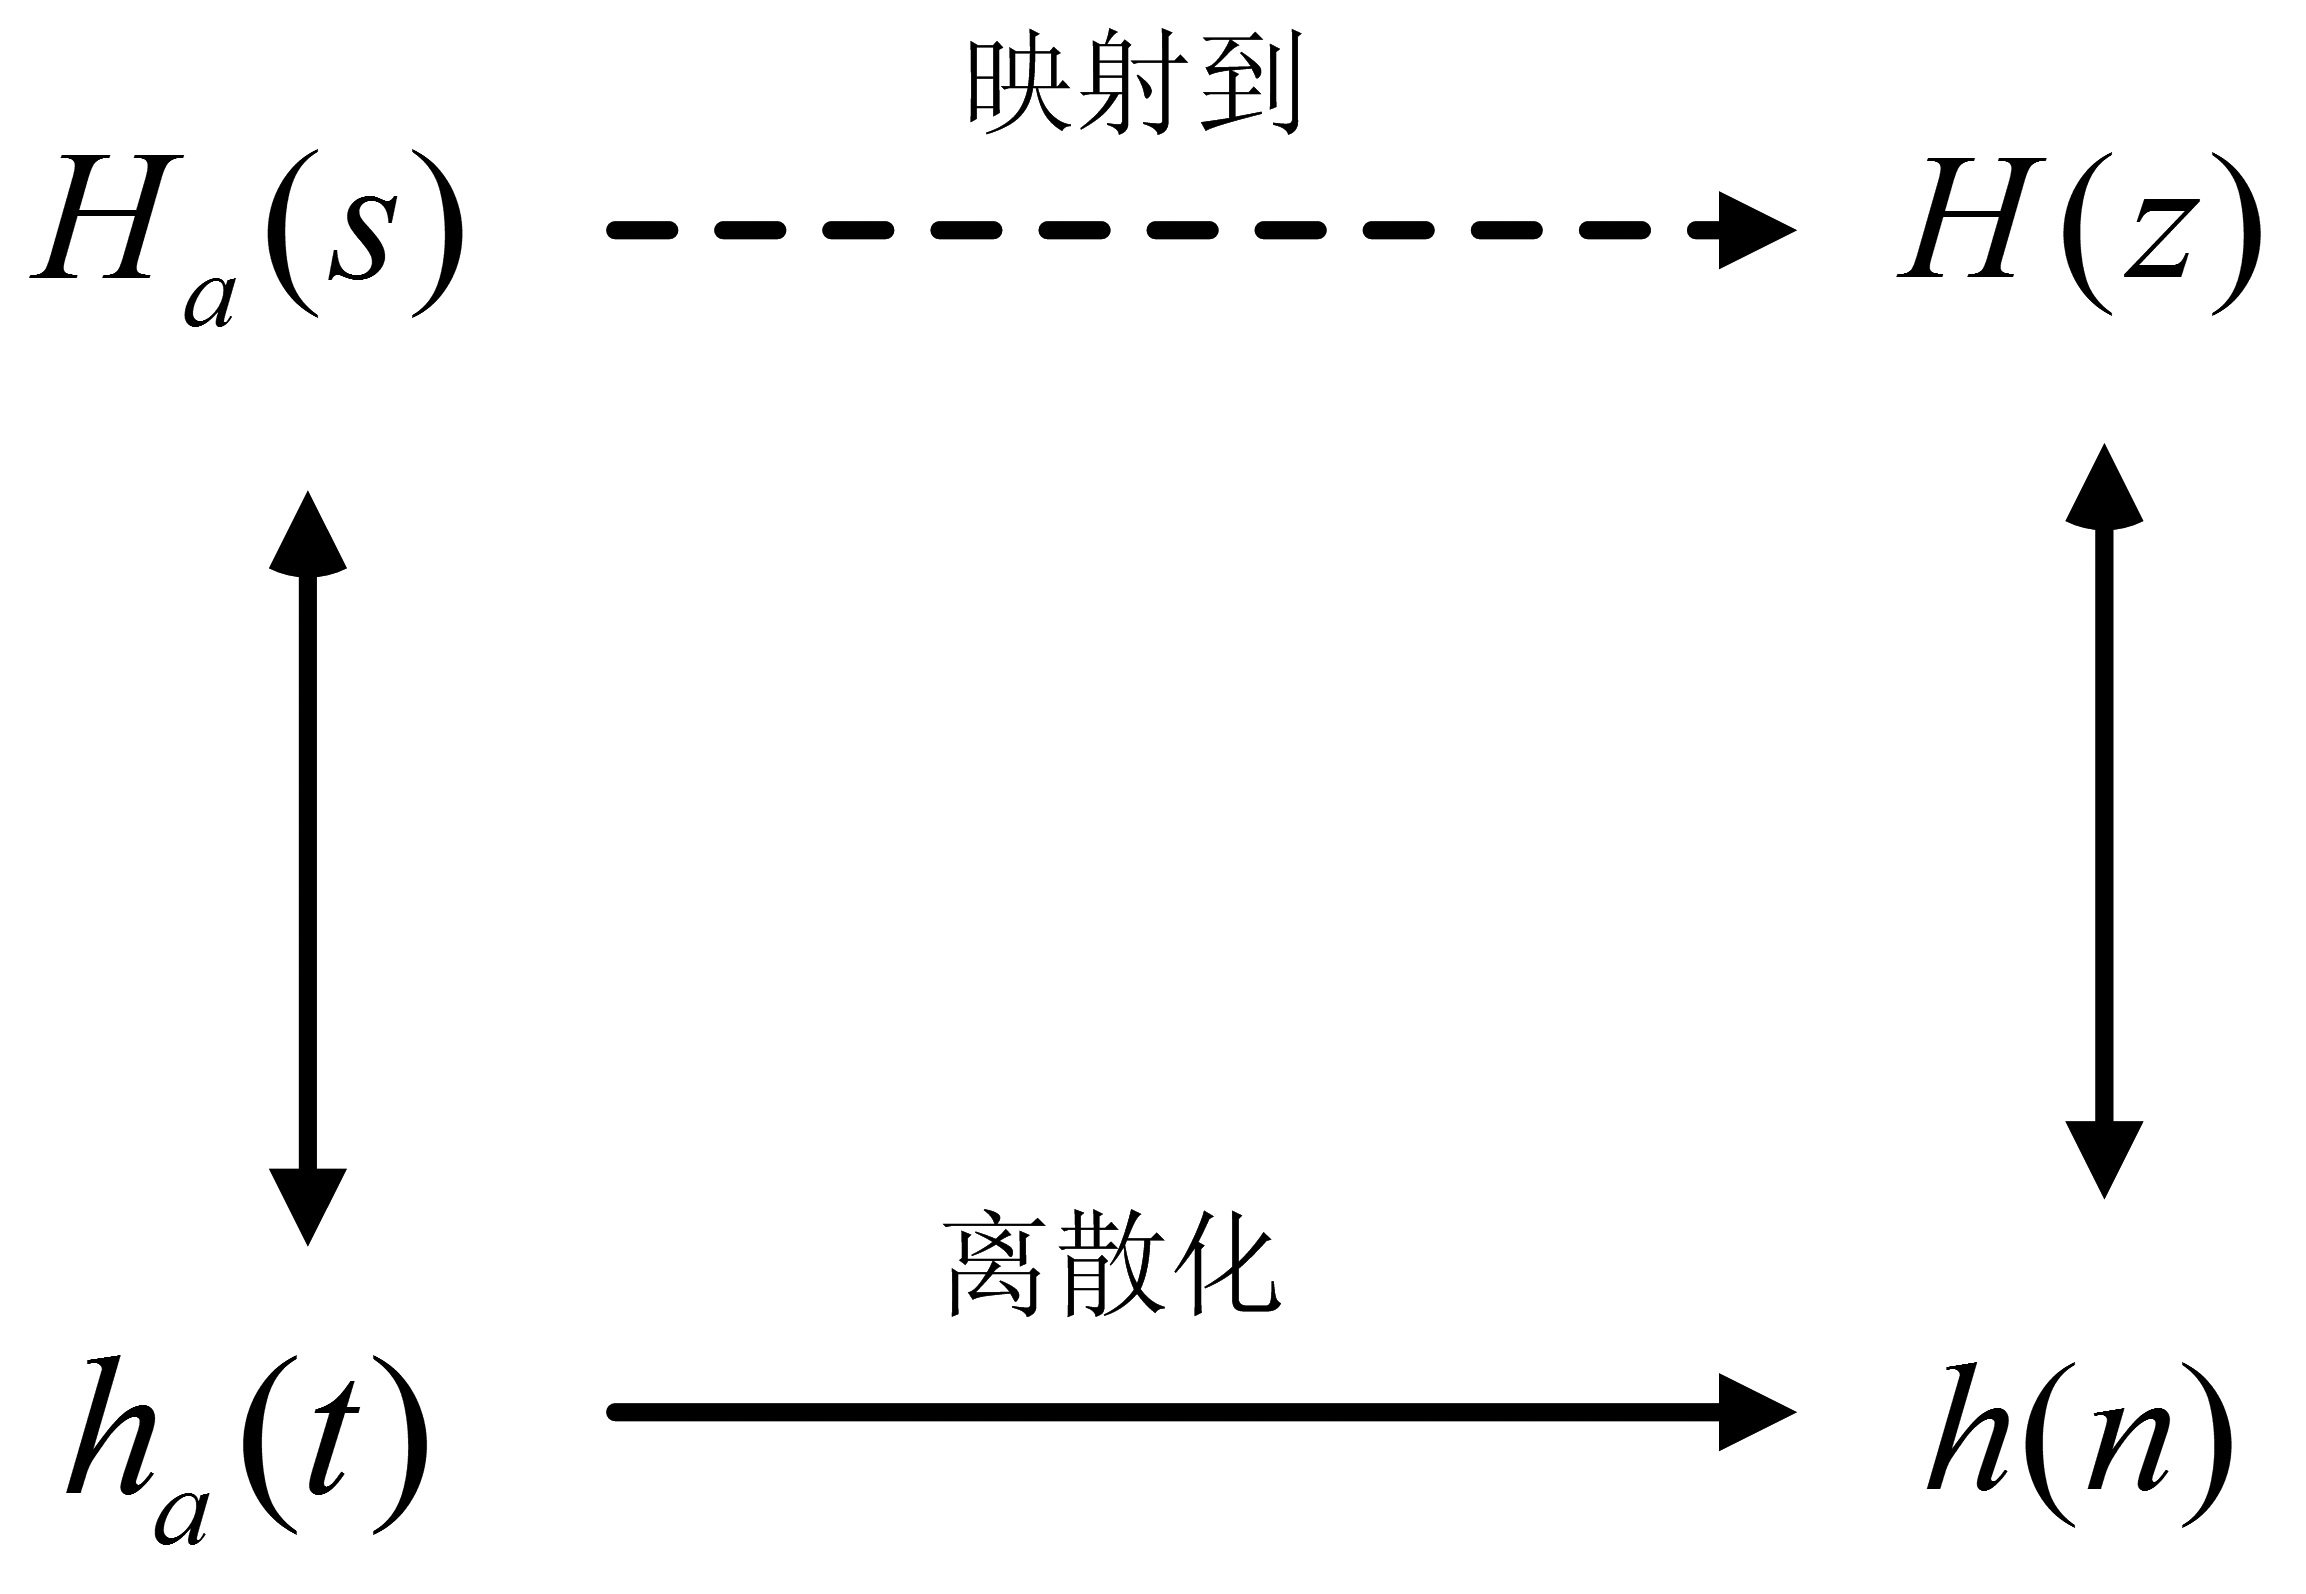
\includegraphics[width=0.45\textwidth]{fig12_maichongxiangying.jpg}
    %\caption{脉冲响应不变法示意图}
    %\vspace{-0.6cm}
    %\label{}
  \end{figure}
\end{frame}
%%%%%%%%%%%%%%%%%%%%%%%%%%%%%%%%%%%%%%%%%%%%%%%%%%%%%%%%%%%%%%%%%%%%%%%%%%%%%%%%%%%%%%%%%%%%%%


%%%%%%%%%%%%%%%%%%%%%%%%%%%%%%%%%%%%%%%%%%%%%%%%%%%%%%%%%%%%%%%%%%%%%%%%%%%%%%%%%%%%%%%%%%%%%%
\begin{frame}[shrink]\frametitle{}%[allowframebreaks][shrink]
\par 设$H_a(s)$只有单阶极点,即:
       $$H_a(s)= \sum_{i=1}^{M}\frac{A_i}{s-s_i}$$
\begin{enumerate}
  \item [1] $H_a(s)\longrightarrow h_a(t)$  (利用拉氏反变换)

        $$\mbox{显然有:}\quad h_a(t) = LT^{-1}[H_a(s)] \quad\quad\quad\quad\quad\quad\quad\quad\quad$$
        $$
        \mbox{且:}\quad\quad \frac{1}{s-s_0}\longleftrightarrow e^{s_{0}t}\mu(t)\quad
        \quad\quad\quad\quad\quad\quad\quad\quad$$
        %\pause
        \begin{dablock}
        $$h_a(t) = LT^{-1}[H_a(s)]= \sum_{i=1}^{M}A_{i}e^{s_{i}t}\mu(t)$$
        \end{dablock}
%        \pause
%  \item [2] $h_a(t)\longrightarrow h(n)$\quad\quad (离散化)
%    $$\mbox{我们知道:}  \quad\quad x(n)=x_a(t)|_{t=nT} = x_a(nT)\quad\quad\quad\quad$$
%    \pause
%    $$\mbox{则:}\quad\quad\quad h(n)=h_a(nT)= \sum_{i=1}^{M}A_{i}e^{s_{i}nT}\mu(nT)
%    \quad$$
\end{enumerate}
\end{frame}
%%%%%%%%%%%%%%%%%%%%%%%%%%%%%%%%%%%%%%%%%%%%%%%%%%%%%%%%%%%%%%%%%%%%%%%%%%%%%%%%%%%%%%%%%%%%%%


%%%%%%%%%%%%%%%%%%%%%%%%%%%%%%%%%%%%%%%%%%%%%%%%%%%%%%%%%%%%%%%%%%%%%%%%%%%%%%%%%%%%%%%%%%%%%%
\begin{frame}[shrink]\frametitle{}%[allowframebreaks]
\begin{enumerate}
    \item [2] $h_a(t)\longrightarrow h(n)$%\quad(h_a(nT))$
\end{enumerate}
    前述可得:
    $$h_a(t) = \sum_{i=1}^{M}A_{i}e^{s_{i}t}\mu(t)$$
    $$\mbox{我们知道:}  \quad\quad x(n)=x_a(t)|_{t=nT} = x_a(nT)\quad\quad\quad\quad$$
    \quad\quad 令 $t=nT$
    %\pause
    \begin{dablock}
    $$\mbox{则:}\quad\quad\quad h(n)=h_a(nT)= \sum_{i=1}^{M}A_{i}e^{s_{i}nT}\mu(nT)
    \quad$$
    \end{dablock}
\end{frame}
%%%%%%%%%%%%%%%%%%%%%%%%%%%%%%%%%%%%%%%%%%%%%%%%%%%%%%%%%%%%%%%%%%%%%%%%%%%%%%%%%%%%%%%%%%%%%%
%
%
%%%%%%%%%%%%%%%%%%%%%%%%%%%%%%%%%%%%%%%%%%%%%%%%%%%%%%%%%%%%%%%%%%%%%%%%%%%%%%%%%%%%%%%%%%%%%%
\begin{frame}[shrink]\frametitle{}%[allowframebreaks]
\begin{enumerate}
    \item [3] $h(n)\longrightarrow H(z)$
    \begin{equation*}
        \begin{split}
            H(z) &= ZT[h(n)]= ZT\left[\sum_{i=1}^{M}A_{i}e^{s_{i}nT}\mu(nT)\right]\\
            &= \sum_{i=1}^{M}A_{i}ZT\left[\left(e^{s_{i}T}\right)^n\mu(n)\right]
            %= \sum_{i=1}^{M}A_{i}\left[\sum_{n=0}^{\infty}(e^{s_{i}T})^{n}z^{-n}\right]\\
        \end{split}
    \end{equation*}
    $$\mbox{我们知道:}\quad\quad a^n\mu(n)\longleftrightarrow \frac{1}{1-az^{-1}}
    \quad\quad\quad\quad\quad\quad\quad\quad$$
    \par\quad  令$a= e^{s_{i}T}$,可得:
    \begin{dablock}
    $$\quad H(z) = \sum_{i=1}^{M}\frac{A_{i}}{1-e^{s_{i}T}z^{-1}}$$
    \end{dablock}
\end{enumerate}
\end{frame}
%%%%%%%%%%%%%%%%%%%%%%%%%%%%%%%%%%%%%%%%%%%%%%%%%%%%%%%%%%%%%%%%%%%%%%%%%%%%%%%%%%%%%%%%%%%%%%
%
%
%%%%%%%%%%%%%%%%%%%%%%%%%%%%%%%%%%%%%%%%%%%%%%%%%%%%%%%%%%%%%%%%%%%%%%%%%%%%%%%%%%%%%%%%%%%%%%
\begin{frame}[shrink]\frametitle{}%[allowframebreaks]
\textbf{利用脉冲响应不变法映射的步骤}
\begin{enumerate}
\item $H_a(s)$进行因式分解,得到标准形式。
      \par 例如:
      $$ H_{a}(s) = \frac{\Omega_{c}^{N}}{\prod^{N-1}_{k=0}(s-s_{k})}  \longrightarrow H_a(s)= \sum_{i=1}^{M}\frac{A_i}{s-s_i}$$
\item 套公式。
      $$H_a(s)= \sum_{i=1}^{M}\frac{A_i}{s-s_i}\longrightarrow H(z) = \sum_{i=1}^{M}\frac{A_{i}}{1-e^{s_{i}T}z^{-1}}$$
\end{enumerate}
\end{frame}
%%%%%%%%%%%%%%%%%%%%%%%%%%%%%%%%%%%%%%%%%%%%%%%%%%%%%%%%%%%%%%%%%%%%%%%%%%%%%%%%%%%%%%%%%%%%%%
%
%
%%%%%%%%%%%%%%%%%%%%%%%%%%%%%%%%%%%%%%%%%%%%%%%%%%%%%%%%%%%%%%%%%%%%%%%%%%%%%%%%%%%%%%%%%%%%%%
\begin{frame}[shrink]\frametitle{}%[allowframebreaks]
%映射关系的讨论
三、映射关系的讨论
\begin{dablock}
已知映射方式为:
$$H_a(s)= \sum_{i=1}^{M}\frac{A_i}{s-s_i}\longrightarrow H(z) = \sum_{i=1}^{M}\frac{A_{i}}{1-e^{s_{i}T}z^{-1}}$$

问题在于: $H_a(s)$与$H(z)$之间的映射关系,也就是说,如何沟通$H_a(s)$与$H(z)$。
\end{dablock}
%\pause
\begin{jytg}
\begin{enumerate}
\item [1] $H_a(s)$与$H(z)$的关系
       \begin{enumerate}
         \item[(a)] $H_a(s)$与$\hat{H}_a(s)$\par
         \item[(b)] $\hat{H}_a(s)$与$H(z)$
       \end{enumerate}
\item [2] 讨论
\end{enumerate}
\end{jytg}
\end{frame}
%%%%%%%%%%%%%%%%%%%%%%%%%%%%%%%%%%%%%%%%%%%%%%%%%%%%%%%%%%%%%%%%%%%%%%%%%%%%%%%%%%%%%%%%%%%%%%
%
%
%%%%%%%%%%%%%%%%%%%%%%%%%%%%%%%%%%%%%%%%%%%%%%%%%%%%%%%%%%%%%%%%%%%%%%%%%%%%%%%%%%%%%%%%%%%%%%
\begin{frame}[shrink]\frametitle{}%[allowframebreaks]
%\begin{enumerate}
%    \item [1] $H_a(s)$与$H(z)$的关系\par
%\end{enumerate}
\begin{enumerate}
    \item[(a)] $H_a(s)$与$\hat{H}_a(s)$\par
        设
        $$h_a(t)\longleftrightarrow H_a(j\Omega)$$
        $$\hat{h}_a(t)\longleftrightarrow \hat{H}_a(j\Omega)$$
        根据采样定理,
        $$\hat{H}_a(j\Omega) = \frac{1}{T}
        \sum_{r=-\infty}^{\infty}H_a(j\Omega-j\frac{2\pi}{T}r)$$
        %\quad\quad\mbox{(采样定理)}
        令 $s=j\Omega$,可得:
        \begin{dablock}
        $$\hat{H}_a(s) = \frac{1}{T}
        \sum_{r=-\infty}^{\infty}H_a(s-j\frac{2\pi}{T}r)$$
        \end{dablock}
\end{enumerate}


\end{frame}
%%%%%%%%%%%%%%%%%%%%%%%%%%%%%%%%%%%%%%%%%%%%%%%%%%%%%%%%%%%%%%%%%%%%%%%%%%%%%%%%%%%%%%%%%%%%%%
%
%
%%%%%%%%%%%%%%%%%%%%%%%%%%%%%%%%%%%%%%%%%%%%%%%%%%%%%%%%%%%%%%%%%%%%%%%%%%%%%%%%%%%%%%%%%%%%%%
\begin{frame}[shrink]\frametitle{}%[allowframebreaks]
\begin{enumerate}
    \item[(b)] $\hat{H}_a(s)$与$H(z)$
\end{enumerate}
            \begin{equation*}
              \begin{split}
                \hat{h}_a(t) &=\sum_{n=-\infty}^{\infty}h_a(t)\delta(t-nT)
                             =\sum_{n=-\infty}^{\infty}h_a(nT)\delta(t-nT)\\
                             &=\sum_{n=-\infty}^{\infty}h(n)\delta(t-nT)\\
              \end{split}
            \end{equation*}
            % dd
            \begin{equation*}
              \begin{split}
            \mbox{又:}\quad     \hat{H}_a(s)
                     &= LT[\hat{h}_a(t)]
                      =\int_{-\infty}^{\infty}\hat{h}_a(t)e^{-st}dt\quad\quad\quad\quad\quad\quad\\
                     &=\int_{-\infty}^{\infty}\left[
                            \sum_{n=-\infty}^{\infty}h(n)\delta(t-nT)\right]e^{-st}dt\\
                     &=\sum_{n=-\infty}^{\infty}h(n)\int_{-\infty}^{\infty}
                             \delta(t-nT)e^{-st}dt\\
                     &= \sum_{n=-\infty}^{\infty}h(n)e^{-snT} =H(z)|_{z=e^{sT}}
              \end{split}
            \end{equation*}
\end{frame}
%%%%%%%%%%%%%%%%%%%%%%%%%%%%%%%%%%%%%%%%%%%%%%%%%%%%%%%%%%%%%%%%%%%%%%%%%%%%%%%%%%%%%%%%%%%%%%
%
%
%%%%%%%%%%%%%%%%%%%%%%%%%%%%%%%%%%%%%%%%%%%%%%%%%%%%%%%%%%%%%%%%%%%%%%%%%%%%%%%%%%%%%%%%%%%%%%
\begin{frame}[shrink]\frametitle{}%[allowframebreaks]
%\begin{enumerate}
\begin{explain}
 注意:分配函数的取样性质:
 $$\int_{-\infty}^{\infty}f(t)\delta(t-t_0)dt = f(t_0)$$
 令$f(t) = e^{-st},t_0 =nT $,可得:
 $$\int_{-\infty}^{\infty}\delta(t-nT)e^{-st}dt = e^{-snT}$$
  \begin{equation*}
  \begin{split}
  \hat{H}_a(s) &=\sum_{n=-\infty}^{\infty}h(n)\int_{-\infty}^{\infty}\delta(t-nT)e^{-st}dt\\
               &= \sum_{n=-\infty}^{\infty}h(n)e^{-snT} =H(z)|_{z=e^{sT}}
  \end{split}
  \end{equation*}
 \end{explain}
 %$$\therefore\quad\quad \hat{H}_a(s)= \sum_{n=-\infty}^{\infty}h(n)e^{-snT}  = H(z)|_{z=e^{sT}}$$
 $\mbox{即:}$
 $$\quad\quad \hat{H}_a(s)= H(z)|_{z=e^{sT}}$$
 %$$\quad\quad\quad  H(z) = \hat{H}_a(s)|_{z=e^{sT}}\quad\quad\quad\quad\quad\quad\quad\quad\quad$$
% $$\mbox{前述有:}\quad \hat{H}_a(s) = \frac{1}{T}\sum_{r=-\infty}^{\infty}H_a(s-j\frac{2\pi}{T}r)
% \quad\quad\quad\quad\quad\quad\quad\quad$$
 %
 %联立两者可得:
% %\pause
% \begin{dablock}
% $$
% H(z)|_{z=e^{sT}}=  \frac{1}{T} \sum_{r=-\infty}^{\infty}H_a(s-j\frac{2\pi}{T}r)
% $$
% \end{dablock}
\end{frame}
%%%%%%%%%%%%%%%%%%%%%%%%%%%%%%%%%%%%%%%%%%%%%%%%%%%%%%%%%%%%%%%%%%%%%%%%%%%%%%%%%%%%%%%%%%%%%%
%
%
%%%%%%%%%%%%%%%%%%%%%%%%%%%%%%%%%%%%%%%%%%%%%%%%%%%%%%%%%%%%%%%%%%%%%%%%%%%%%%%%%%%%%%%%%%%%%%
\begin{frame}[allowframebreaks]\frametitle{}%[allowframebreaks]
%\begin{enumerate}
%
% 注意:分配函数的取样性质:
% $$\int_{-\infty}^{\infty}f(t)\delta(t-t_0)dt = f(t_0)$$
% $$\therefore\quad\quad \hat{H}_a(s)= \sum_{n=-\infty}^{\infty}h(n)e^{-snT}  = H(z)|_{z=e^{sT}}$$
 \quad 通过上述推导可知:
 $$\mbox{}\quad\quad\quad   \hat{H}_a(s)= H(z)|_{z=e^{sT}}\quad\quad\quad\quad\quad\quad\quad\quad\quad$$
 $$\mbox{前述有:}\quad \hat{H}_a(s) = \frac{1}{T}\sum_{r=-\infty}^{\infty}H_a(s-j\frac{2\pi}{T}r)
 \quad\quad\quad\quad\quad\quad\quad\quad$$
 %
 联立两者可得:
 %\pause
 \begin{dablock}
 $$
 H(z)|_{z=e^{sT}}=  \frac{1}{T}          \sum_{r=-\infty}^{\infty}H_a(s-j\frac{2\pi}{T}r)
 $$
 \end{dablock}
\end{frame}
%%%%%%%%%%%%%%%%%%%%%%%%%%%%%%%%%%%%%%%%%%%%%%%%%%%%%%%%%%%%%%%%%%%%%%%%%%%%%%%%%%%%%%%%%%%%%%
%
%
%%%%%%%%%%%%%%%%%%%%%%%%%%%%%%%%%%%%%%%%%%%%%%%%%%%%%%%%%%%%%%%%%%%%%%%%%%%%%%%%%%%%%%%%%%%%%%
\begin{frame}[shrink]\frametitle{2 讨论}%[allowframebreaks][shrink]
\begin{jytg}
\begin{enumerate}
    \item [1] $H_a(s)$与$H(z)$的关系:
        \begin{enumerate}
            \item [(1)]  $H_a(s)$与$\hat{H}_a(s)$
            \item [(2)] $\hat{H}_a(s)$与$H(z)$
        \end{enumerate}
    \item [2] \textbf{讨论}:
        \begin{enumerate}
            \item [(1)] 物理意义
            \item [(2)] 映射关系
            \item [(3)] 结论
        \end{enumerate}
\end{enumerate}
\end{jytg}

%$$H(z)|_{z=e^{sT}}=  \frac{1}{T}\sum_{r=-\infty}^{\infty}H_a(s-j\frac{2\pi}{T}r)$$
%      \begin{enumerate}
%        \item [(1)] 物理意义
%              公式揭示了在脉冲响应不变法的原则下$H_a(s)$与$H(z)$的关系。
%              即:
%              \begin{enumerate}
%                \item[a] 先将$H_a(s)$在s平面虚轴上,以$\Omega_s = \frac{2\pi}{T}$为周期延拓。
%                \item[b] 再按照$z=e^{sT}$关系映射到$H(z)$
%              \end{enumerate}
% \end{enumerate}
\end{frame}
%%%%%%%%%%%%%%%%%%%%%%%%%%%%%%%%%%%%%%%%%%%%%%%%%%%%%%%%%%%%%%%%%%%%%%%%%%%%%%%%%%%%%%%%%%%%%%
%
%
%
%%%%%%%%%%%%%%%%%%%%%%%%%%%%%%%%%%%%%%%%%%%%%%%%%%%%%%%%%%%%%%%%%%%%%%%%%%%%%%%%%%%%%%%%%%%%%%
\begin{frame}[shrink]\frametitle{}%[allowframebreaks][shrink]
$$H(z)|_{z=e^{sT}}=  \frac{1}{T}\sum_{r=-\infty}^{\infty}H_a(s-j\frac{2\pi}{T}r)$$
      \begin{enumerate}
        \item [(1)] 物理意义\par

              公式揭示了在脉冲响应不变法的原则下$H_a(s)$与$H(z)$的关系。
              即:
              \begin{enumerate}
                \item[a] 先将$H_a(s)$在s平面虚轴上,以$\Omega_s = \frac{2\pi}{T}$为周期延拓。
                \item[b] 再按照$z=e^{sT}$关系映射到$H(z)$
              \end{enumerate}
        \item [(2)] 映射关系
        \begin{enumerate}
          \item [a]在数值上:
            \begin{figure}[h]
               \centering
               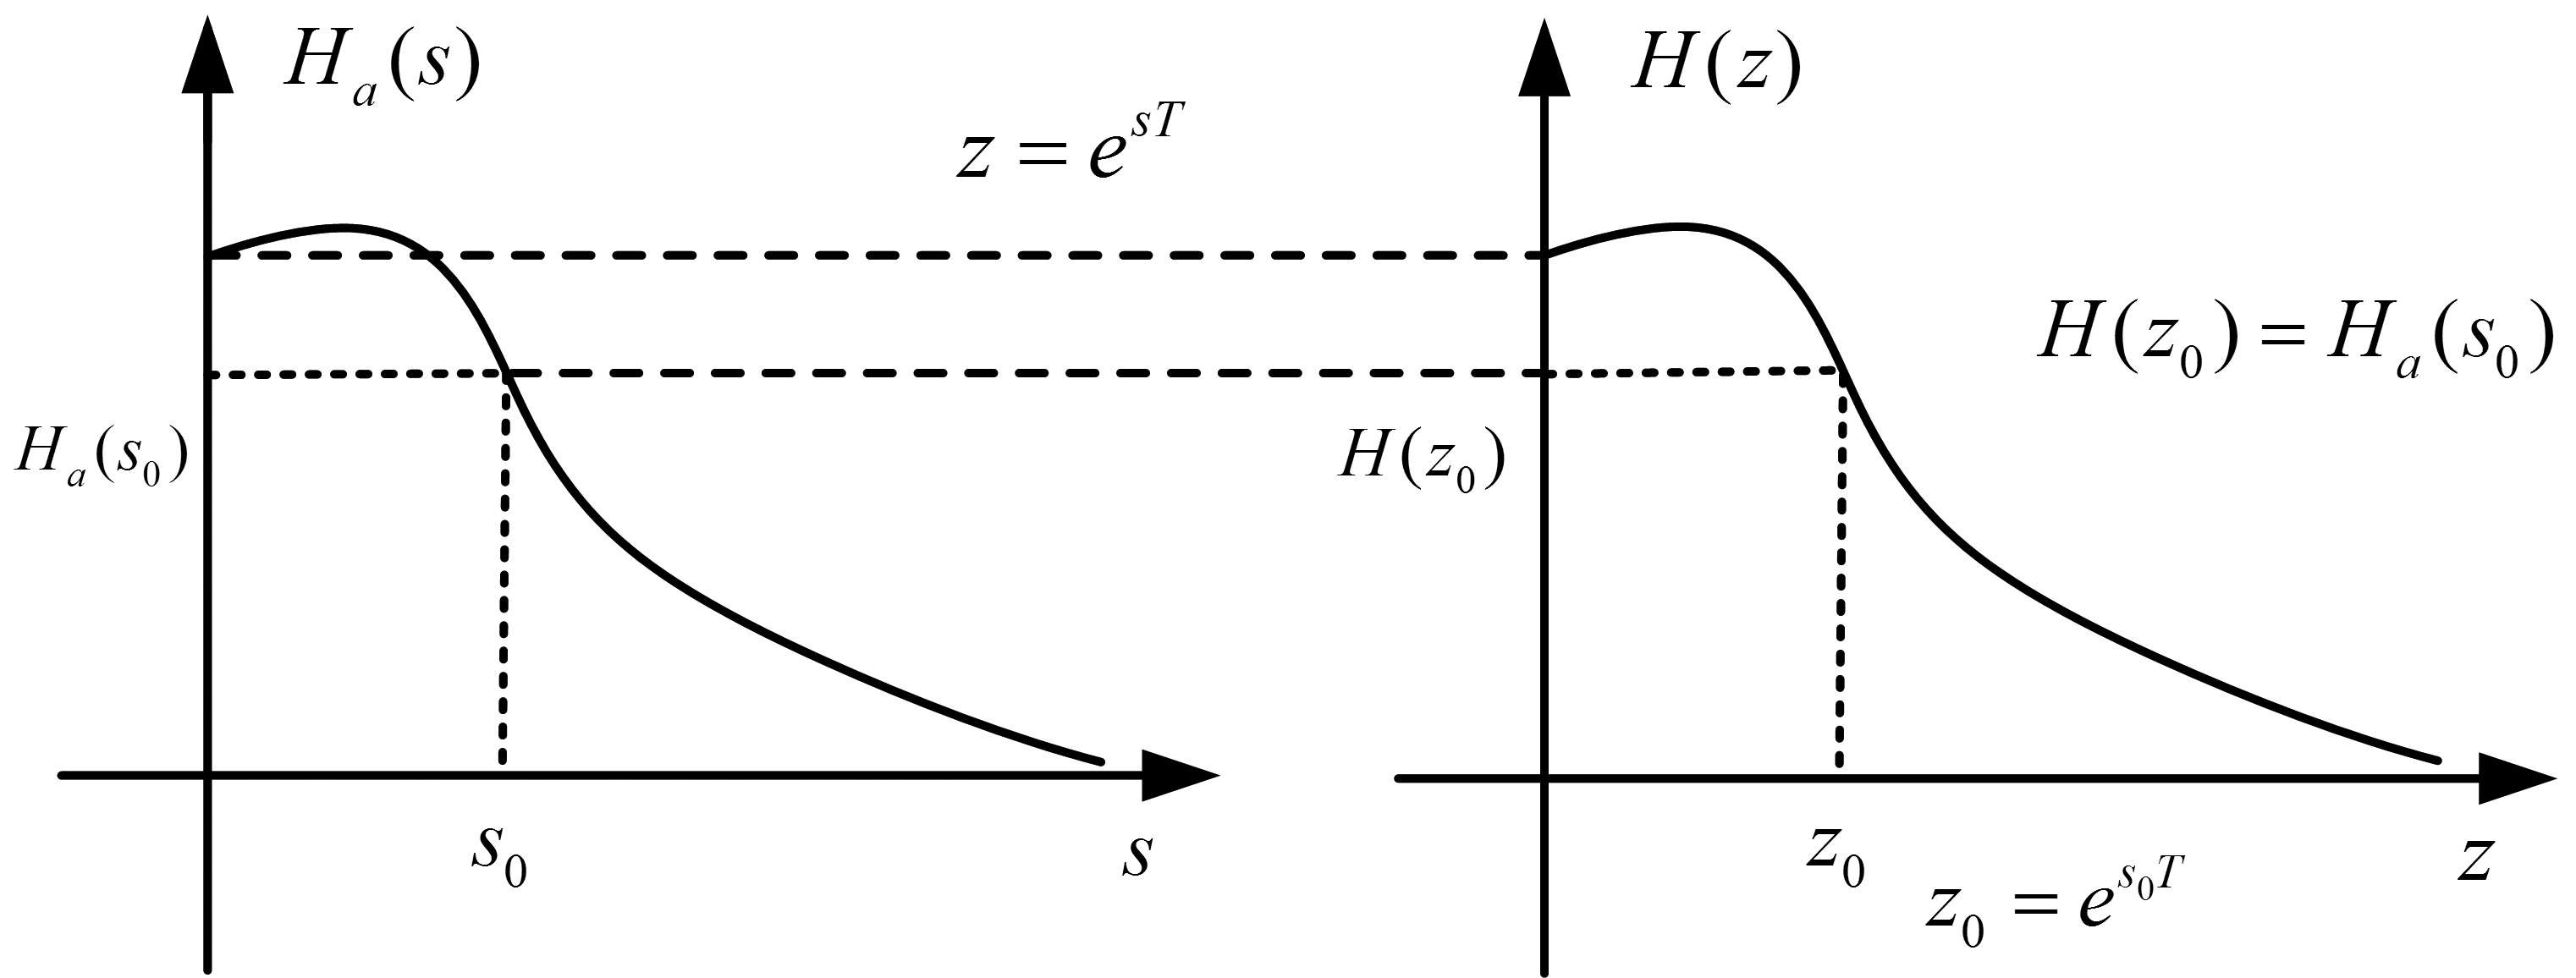
\includegraphics[width=0.6\textwidth]{fig13_MZshuzhiduiying.jpg}
                        %\caption{脉冲响应不变法映射在数值上的对应关系,将二维压缩到一维。}
                        %\label{}
                        %\vspace{-0.7cm}
             \end{figure}
       \end{enumerate}
\end{enumerate}
\end{frame}
%%%%%%%%%%%%%%%%%%%%%%%%%%%%%%%%%%%%%%%%%%%%%%%%%%%%%%%%%%%%%%%%%%%%%%%%%%%%%%%%%%%%%%%%%%%%%%
%
%
%%%%%%%%%%%%%%%%%%%%%%%%%%%%%%%%%%%%%%%%%%%%%%%%%%%%%%%%%%%%%%%%%%%%%%%%%%%%%%%%%%%%%%%%%%%%%
\begin{frame}[shrink]\frametitle{}%[allowframebreaks][shrink]
\begin{enumerate}
\item [b]映射关系为:$\quad\quad z=e^{sT}$
    $$\mbox{设}\quad\quad s=\sigma + j\Omega, \quad\quad\quad z=r\cdot e^{j\omega}$$
    \begin{figure}[h]
        \centering
        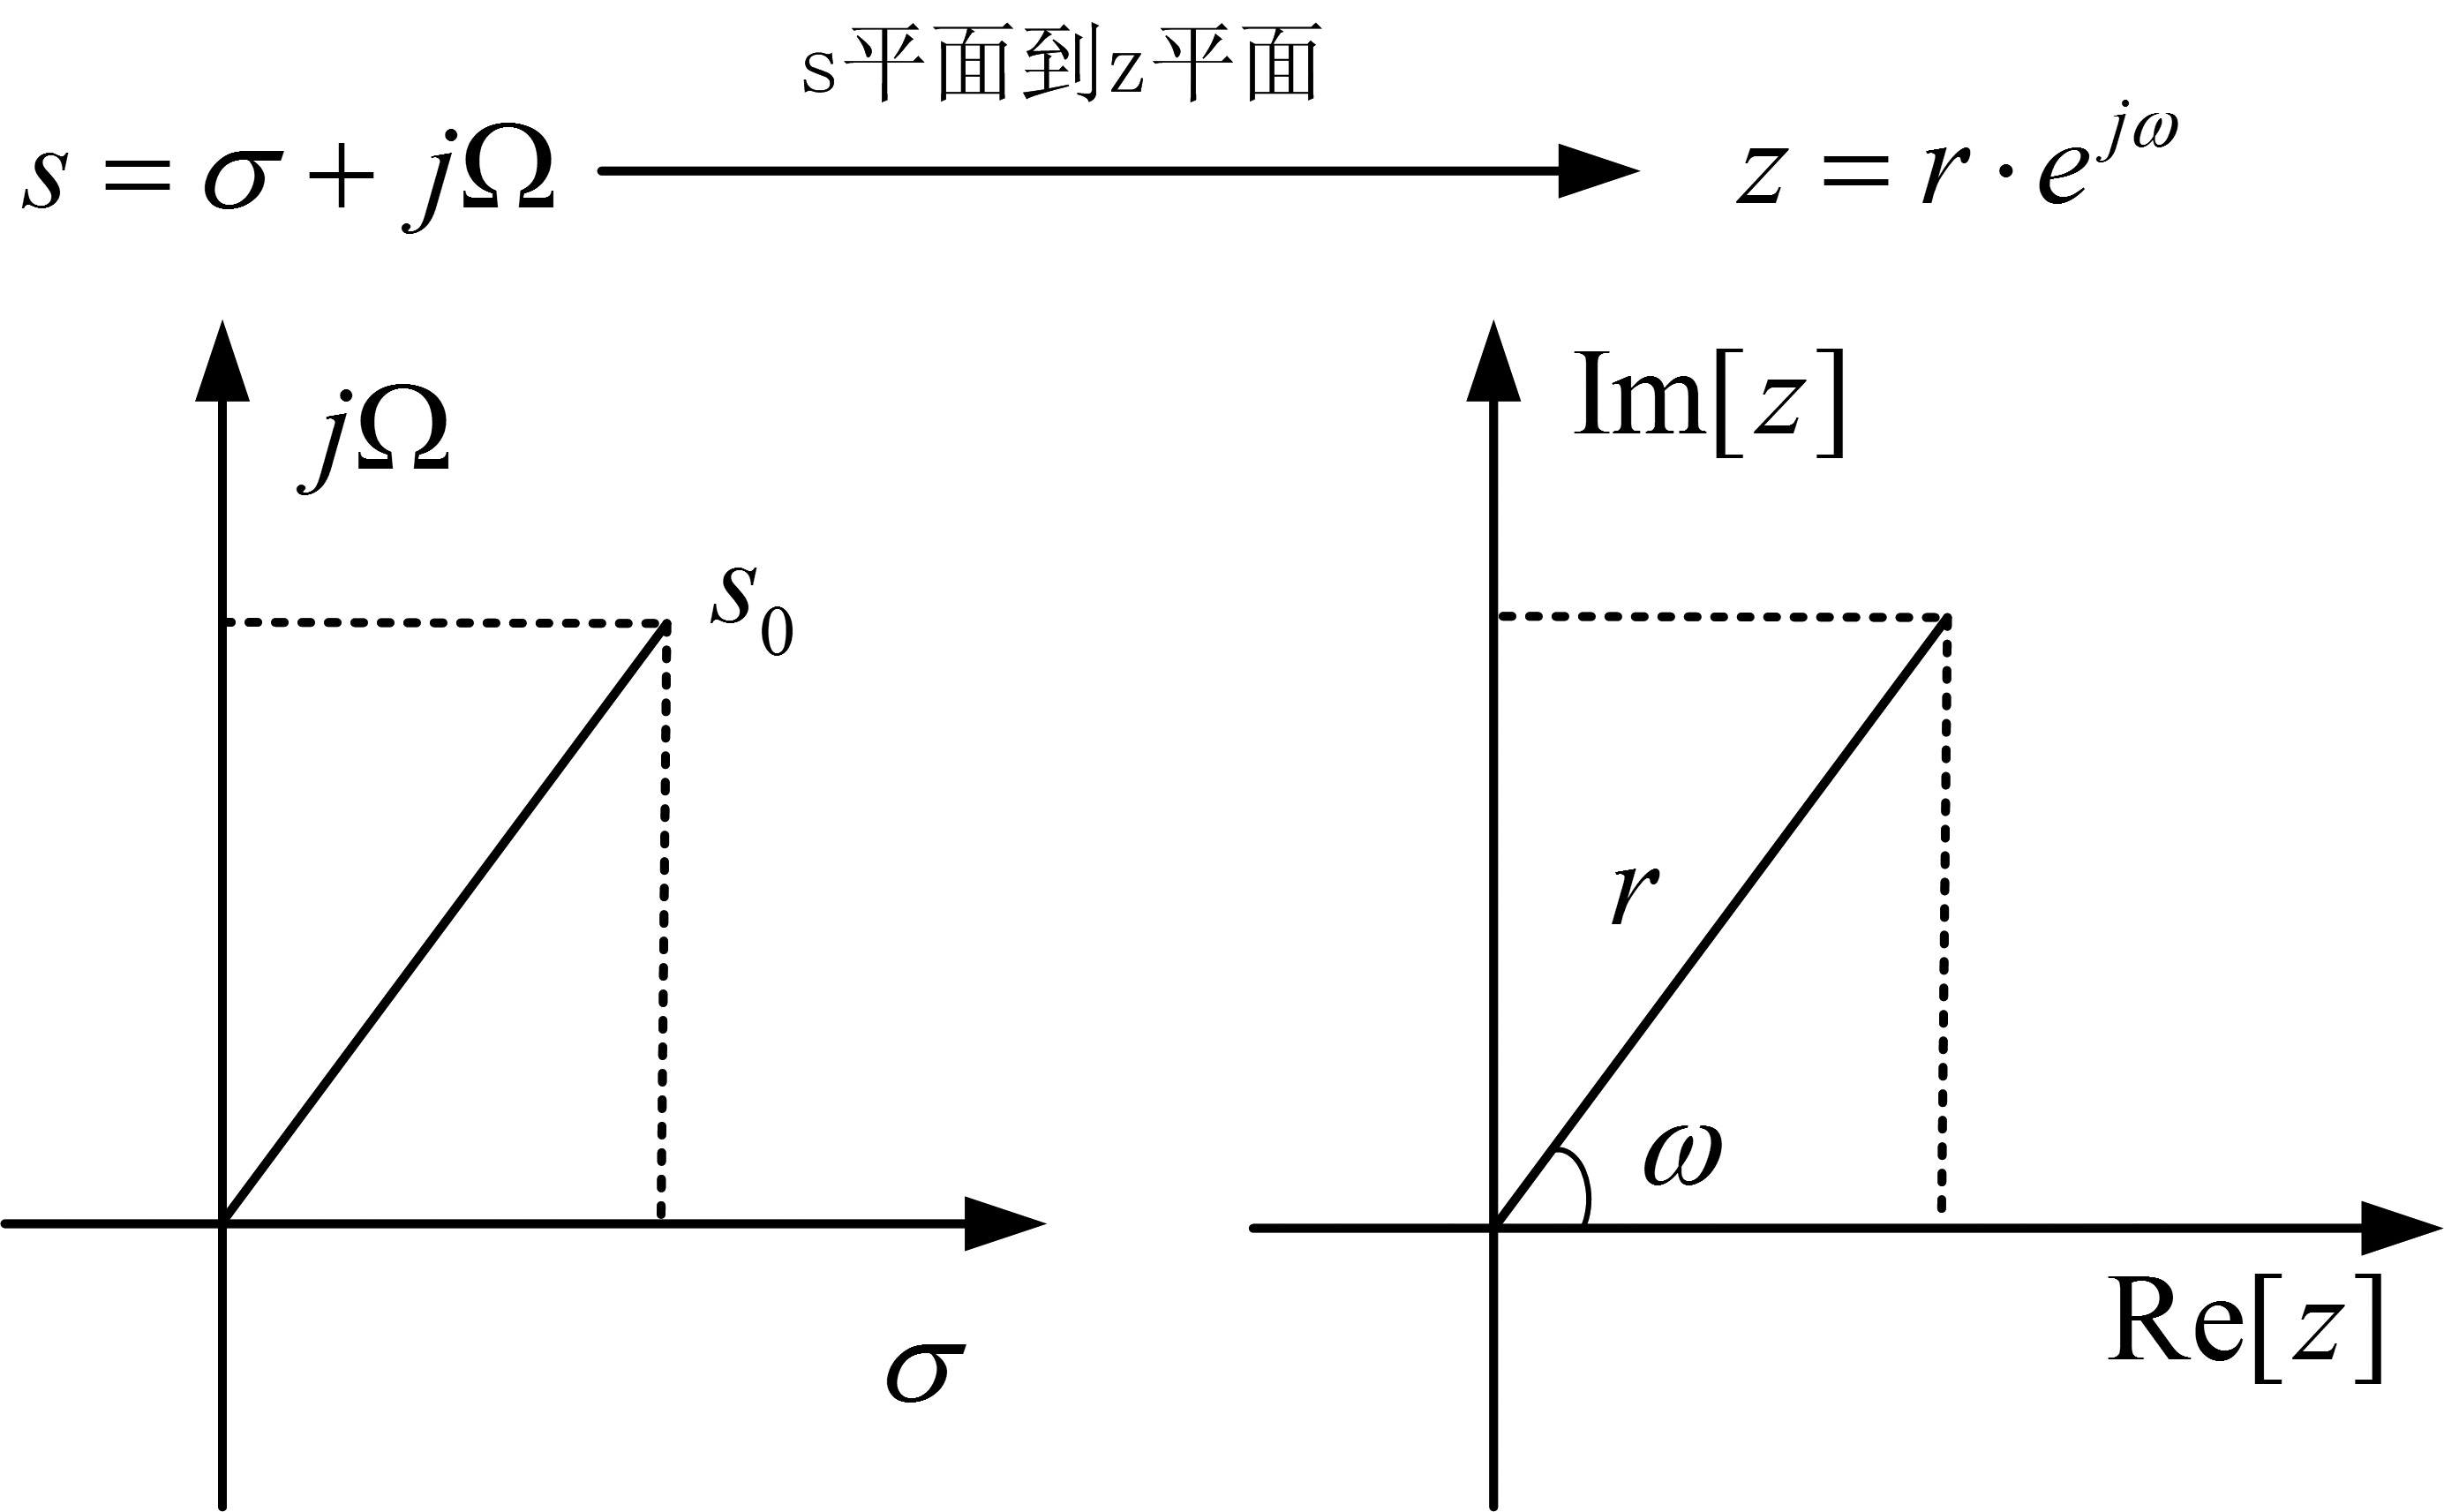
\includegraphics[width=0.6\textwidth]{fig14_MZzhijiaojizuobiao.jpg}
        %\caption{直角坐标到极坐标的示意图。}
        %\label{}
        %\vspace{-0.7cm}
    \end{figure}
    注意:\par
    映射关系为:
    $$z=e^{sT}$$
    Z平面的极坐标表示方式为:
    $$z=re^{j\omega}$$

%    $$re^{j\omega}= e^{sT} = e^{(\sigma+j\Omega)T} = e^{\sigma T}\cdot e^{j\Omega T}
%    = e^{\sigma T}\cdot e^{j(\Omega+\frac{2\pi}{T}M)T}$$                  $$\mbox{即:}\quad\quad r = e^{\sigma T} \quad\quad \omega = \Omega T$$
\end{enumerate}

\end{frame}
%%%%%%%%%%%%%%%%%%%%%%%%%%%%%%%%%%%%%%%%%%%%%%%%%%%%%%%%%%%%%%%%%%%%%%%%%%%%%%%%%%%%%%%%%%%%%%
%
%
%%%%%%%%%%%%%%%%%%%%%%%%%%%%%%%%%%%%%%%%%%%%%%%%%%%%%%%%%%%%%%%%%%%%%%%%%%%%%%%%%%%%%%%%%%%%%%%
\begin{frame}[shrink]\frametitle{}%[allowframebreaks][shrink]
则有:
$$z=re^{j\omega} \qquad\mbox{同时}\qquad z= e^{sT} = e^{(\sigma+j\Omega)T} = e^{\sigma T}\cdot e^{j\Omega T}\qquad $$%= e^{\sigma T}\cdot e^{j(\Omega+\frac{2\pi}{T}M)T}$$
$\mbox{对比可得:}$
\begin{equation*}
  \begin{split}
     r       &= e^{\sigma T} \quad\quad\quad\quad\quad\quad\quad\quad\quad\quad\quad\quad\quad\quad\\
     \omega  &= \Omega T
   \end{split}
\end{equation*}



%$$\mbox{即:}\quad\quad r = e^{\sigma T} \quad\quad \omega = \Omega T$$
%$$\mbox{即:}\quad\quad r = e^{\sigma T} \quad\quad \omega = \Omega T$$


可以看出:
    \begin{enumerate}
        \item 根据$r= e^{\sigma T}$,可知:
            $$
              \left\{
              \begin{aligned}
              \mbox{若$\sigma<0$,则$r<1$$\quad\longrightarrow\quad$
              s左半平面映射到z平面单位圆内。}\\
              \mbox{若$\sigma=0$,则$r=1$$\quad\longrightarrow\quad$
              s平面虚轴映射到z平面单位圆上。}\\
              \mbox{若$\sigma>0$,则$r>1$$\quad\longrightarrow\quad$
              s右半平面映射到z平面单位圆外。}\\
              \end{aligned}
              \right.
            $$
        \item 根据$e^{\sigma T}\cdot e^{j\Omega T} = e^{\sigma T}\cdot e^{j(\Omega+\frac{2\pi}{T}M)T}$,可知:\par
            当$\sigma$不变时,模拟频率$\Omega$变化$\frac{2\pi}{T}$的整数
                          倍时,映射值不变。
    \end{enumerate}

\end{frame}
%%%%%%%%%%%%%%%%%%%%%%%%%%%%%%%%%%%%%%%%%%%%%%%%%%%%%%%%%%%%%%%%%%%%%%%%%%%%%%%%%%%%%%%%%%%%%%
%
%
%%%%%%%%%%%%%%%%%%%%%%%%%%%%%%%%%%%%%%%%%%%%%%%%%%%%%%%%%%%%%%%%%%%%%%%%%%%%%%%%%%%%%%%%%%%%%%
\begin{frame}[shrink]\frametitle{}%[allowframebreaks]
\begin{enumerate}
        \item [(3)]结论
\end{enumerate}
          s平面上任何一个宽度为$\frac{2\pi}{T}$的水平横带区域都一定重复映射到全体
          z平面,且该映射为一多值映射。
           \begin{figure}[h]
           \centering
           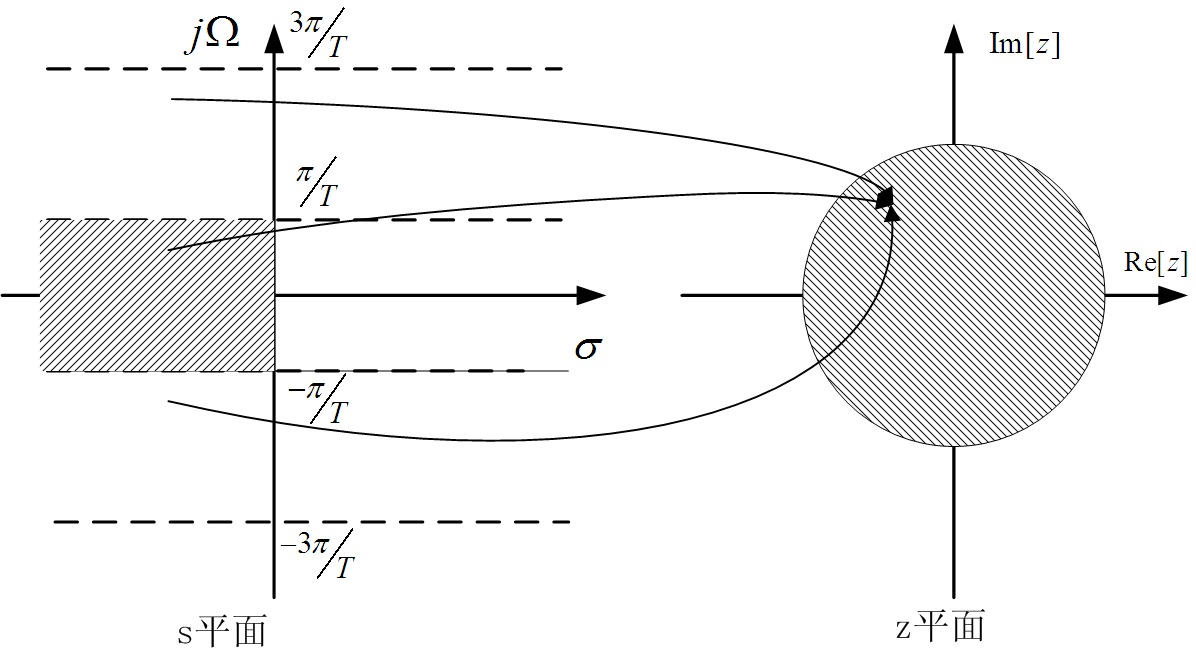
\includegraphics[width=0.75\textwidth]{fig15_MZspinmian2zpingmian.jpg}
           \caption{脉冲响应不变法:s平面到z平面映射关系示意图}
           %\label{}
           %\vspace{-0.8cm}
           \end{figure}

\end{frame}
%%%%%%%%%%%%%%%%%%%%%%%%%%%%%%%%%%%%%%%%%%%%%%%%%%%%%%%%%%%%%%%%%%%%%%%%%%%%%%%%%%%%%%%%%%%%%%
%
%
%%%%%%%%%%%%%%%%%%%%%%%%%%%%%%%%%%%%%%%%%%%%%%%%%%%%%%%%%%%%%%%%%%%%%%%%%%%%%%%%%%%%%%%%%%%%%%
\begin{frame}[allowframebreaks]\frametitle{}%[allowframebreaks]
四、脉冲响应不变法的频率混叠
\begin{enumerate}
  \item [1] 原因

       映射是多值映射,不是单值映射。
        $$
        H(z)|_{z=e^{sT}}= \hat{H}_a(s)  = \frac{1}{T}\sum_{r=-\infty}^{\infty}H_a(s-j\frac{2\pi}{T}r)
        $$
        令 $z=e^{j\omega}\quad$,$s=j\Omega$,可得:
        $$
        H(e^{j\omega})|_{e^{j\omega}=e^{j\Omega T}}%=\hat{H}_a(s)
        =  \frac{1}{T}\sum_{r=-\infty}^{\infty}H_a(j\Omega-j\frac{2\pi}{T}r)
        \quad\quad\quad\quad\quad(1)$$
%        又有:
%        $$\hat{H}_a(j\Omega) = \frac{1}{T}
%            \sum_{r=-\infty}^{\infty}H_a(j\Omega-j\frac{2\pi}{T}r)
%            \quad\quad\mbox{(采样定理)}
%        $$
%
%        $$
%        \mbox{可得:} \quad\quad\quad\quad H(e^{j\omega})|_{\omega=\Omega T}  =  \hat{H}_a(j\Omega)%|_{\Omega=\frac{\omega}{T}}
%        \quad\quad\quad\quad\quad\quad\quad\quad$$
%        改写公式(1)可得:
        则:
        $$
         H(e^{j\omega})|_{\omega=\Omega T}
            =  \frac{1}{T}\sum_{r=-\infty}^{\infty}H_a(j\Omega-j\frac{2\pi}{T}r)
        $$
        \textbf{可见:}
        $H(e^{j\omega})$是$H_a(j\Omega)$以$\frac{2\pi}{T}$为周期在$j\Omega$
        轴上进行延拓后,在频率轴上归一化得到的结果。
        $$H_a(j\Omega)\underrightarrow{\quad\mbox{延拓}\quad}
        \hat{H}_a(j\Omega)\underrightarrow{\quad \omega=\Omega T\quad} H(e^{j\omega})$$


        \begin{figure}[h]
           \centering
           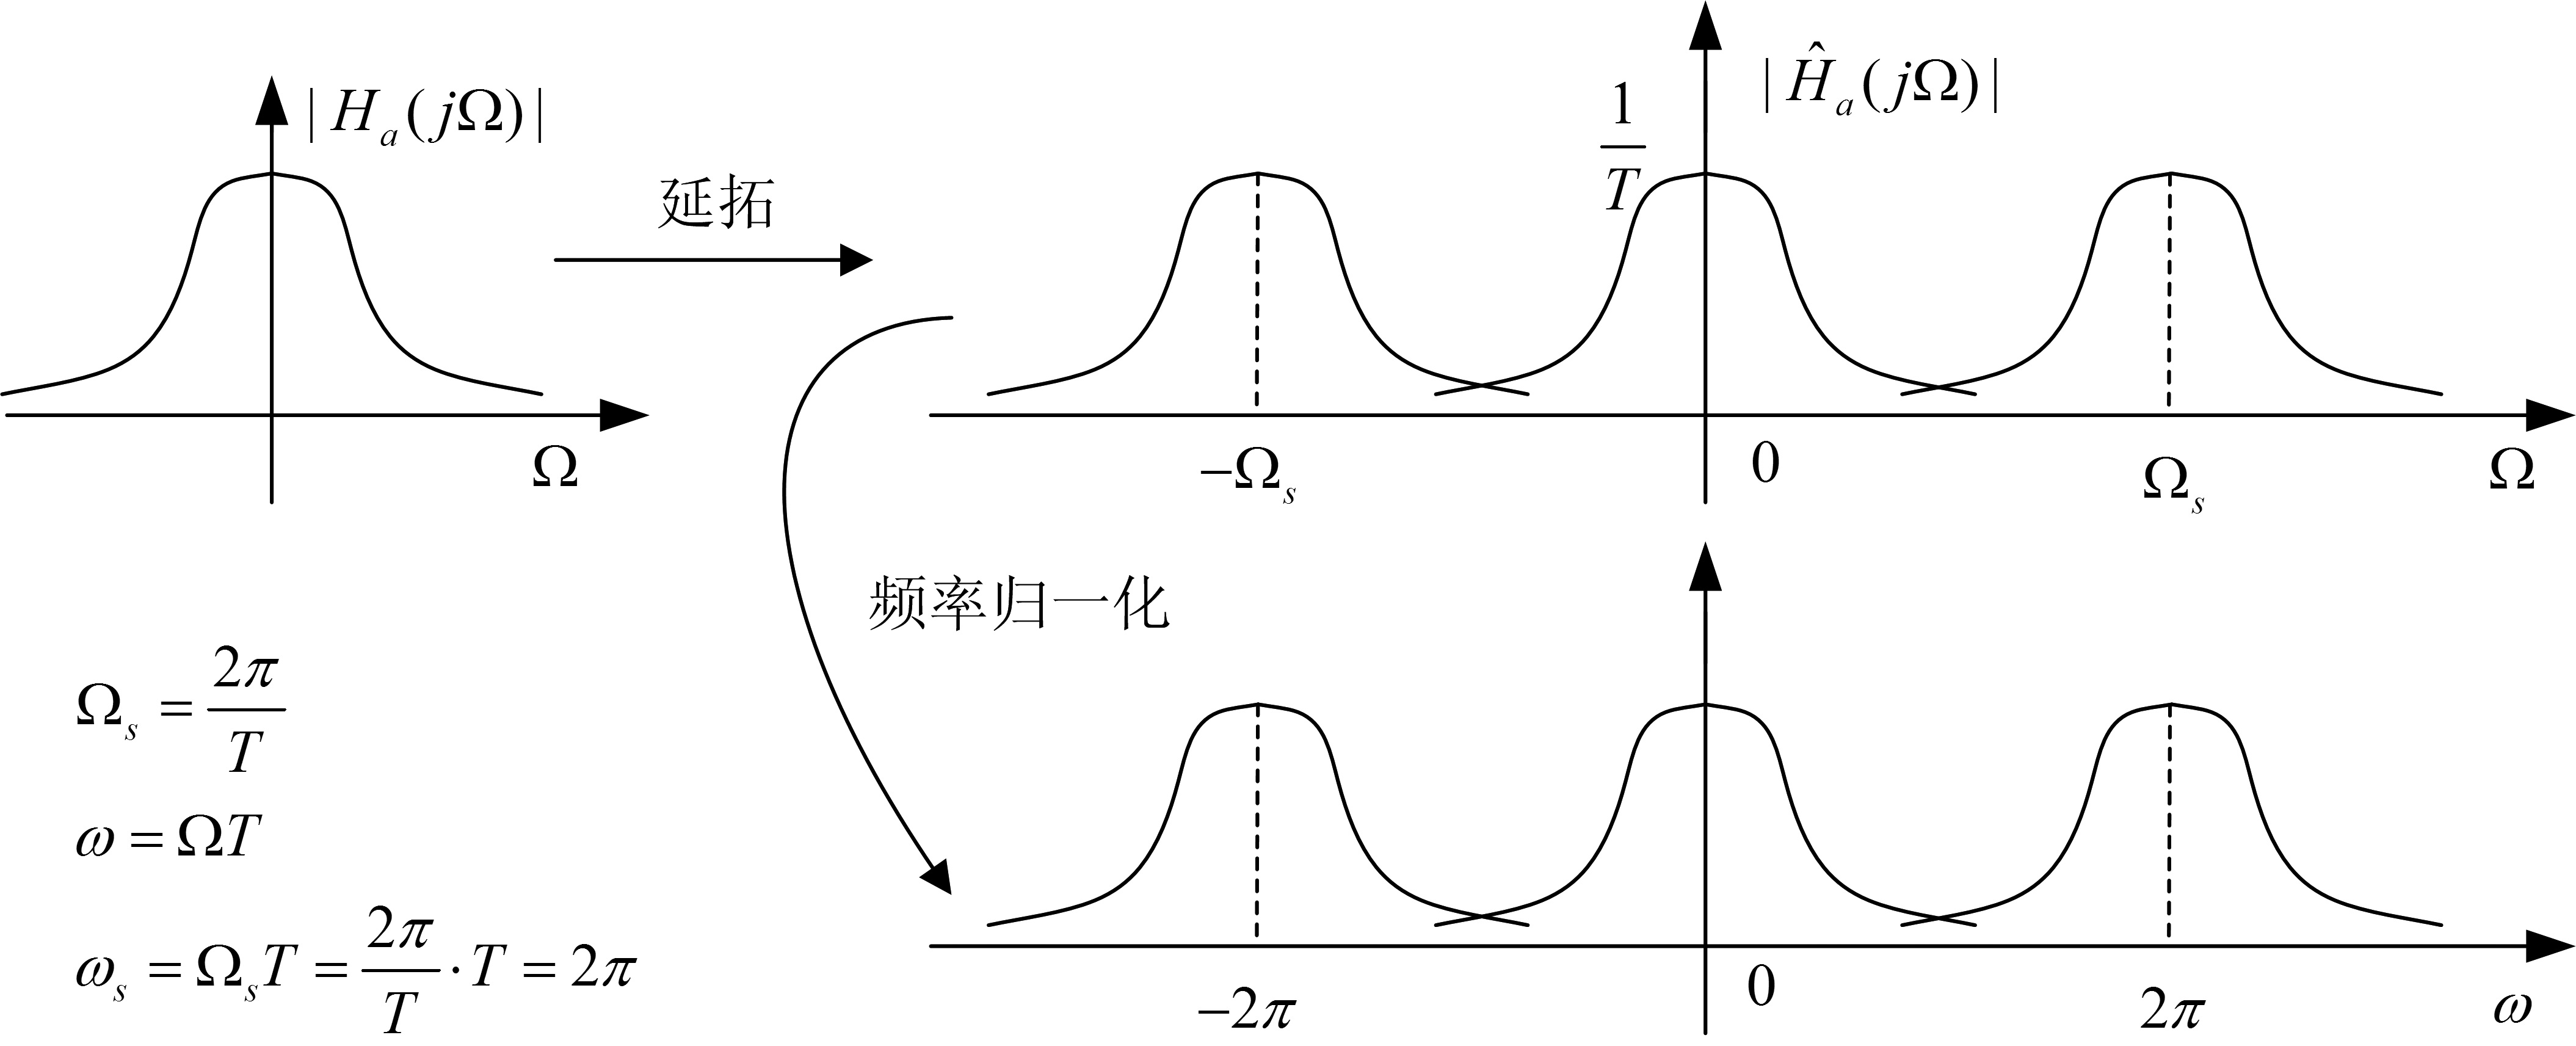
\includegraphics[width=0.9\textwidth]{fig16_MZpinlvhundie.jpg}
           \caption{数字信号与模拟信号频谱关系示意图}
           %\label{}
           %\vspace{-0.2cm}
        \end{figure}
  \newpage
  \item [2] 频谱失真的含义

  \begin{enumerate}
    \item [(1)]
        若$H_a(j\Omega)$为带限信号,即$\frac{2\pi}{T}\geqslant 2\Omega_c(f_s\geqslant2f_c)$,则无重叠,此为理想情况。
    \item [(2)]
        若$H_a(j\Omega)$为非带限信号,即$f_s\leqslant2f_c$,此时的
        $H_a(j\Omega)$在延拓后总存在混叠现象。且在$\frac{\pi}{T}$处
        失真最大,对于数字滤波器,即在$\omega=\pi$处,失真最大。
        \begin{figure}[h]
           \centering
           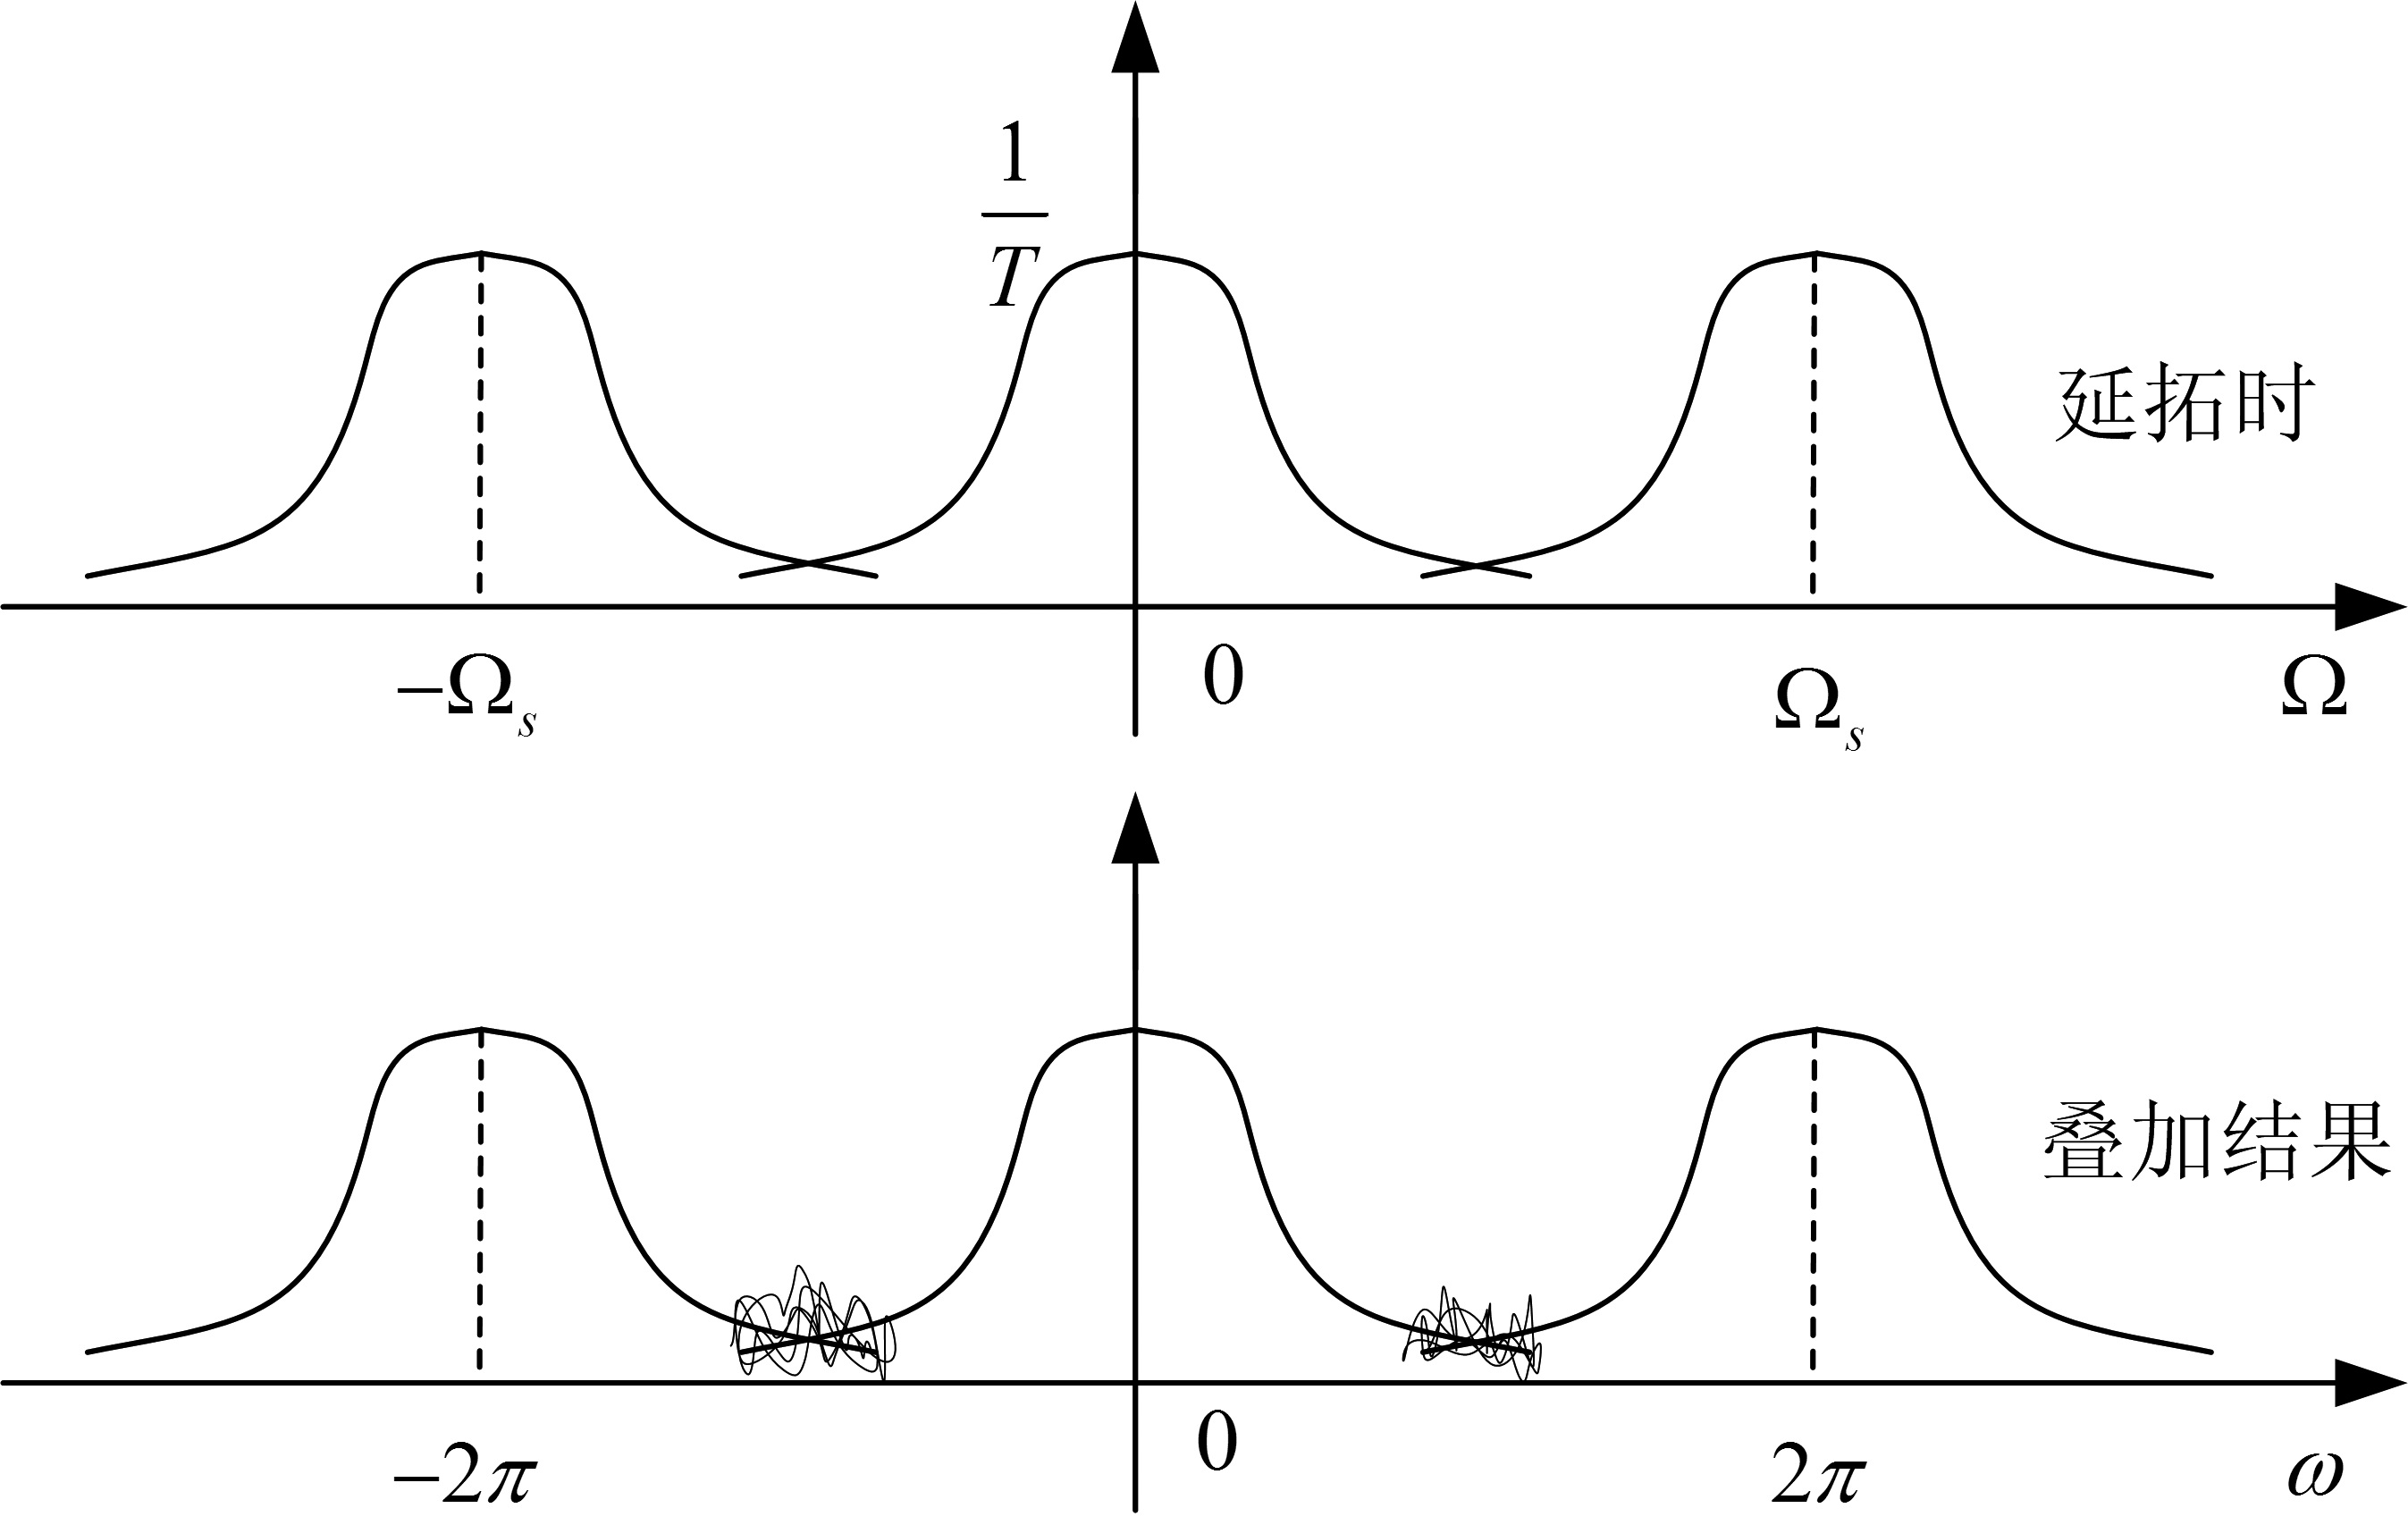
\includegraphics[width=0.55\textwidth]{fig17_MZdiejiajieguo.jpg}
           %\caption{频率混叠现象示意图}
           %\label{}
           %\vspace{-0.3cm}
        \end{figure}

    \item [(3)]
        失真不可避免,因此频率响应不变法\textbf{只能用于设计低通、带通}数字滤波器的设计。\emph{不适合高通、带阻}数字滤波器的设计。
  \end{enumerate}
\end{enumerate}
\end{frame}
%%%%%%%%%%%%%%%%%%%%%%%%%%%%%%%%%%%%%%%%%%%%%%%%%%%%%%%%%%%%%%%%%%%%%%%%%%%%%%%%%%%%%%%%%%%%%%
%
%
%%%%%%%%%%%%%%%%%%%%%%%%%%%%%%%%%%%%%%%%%%%%%%%%%%%%%%%%%%%%%%%%%%%%%%%%%%%%%%%%%%%%%%%%%%%%%%
\begin{frame}\frametitle{}%[allowframebreaks][shrink]
\textbf{五、脉冲响应不变法的优点与缺点}
\begin{enumerate}
  \item [1] 优点:

      \begin{enumerate}
        \item [(1)] 原理简单,${(\omega=\Omega T),\quad\quad(r=e^{\sigma T})}$;
        \item [(2)] 映射前后频率为线性关系。
      \end{enumerate}
  \item [2] 缺点

      非单值映射,存在频率失真,应用范围限制在低通和带通,不适合高通和带阻
      滤波器的设计。
\end{enumerate}
\end{frame}
%%%%%%%%%%%%%%%%%%%%%%%%%%%%%%%%%%%%%%%%%%%%%%%%%%%%%%%%%%%%%%%%%%%%%%%%%%%%%%%%%%%%%%%%%%%%%%%

\section{6.4 IIR-DF的设计—双线性变换法(BLT)}

%%%%%%%%%%%%%%%%%%%%%%%%%%%%%%%%%%%%%%%%%%%%%%%%%%%%%%%%%%%%%%%%%%%%%%%%%%%%%%%%%%%%%%%%%%%%%%
\begin{frame}\frametitle{双线性变换法(BLT)}%[allowframebreaks][shrink]
\begin{itemize}
    \item 脉冲响应不变法主要的缺点是产生了频率混叠
    \item 其原因为:LP-AF不带限于$\frac{\pi}{T}$,离散后在$\omega = \pi$处产生了频率混叠
  \end{itemize}

   直观的想法:
   $$\mbox{将整个模拟轴}\underrightarrow{\quad\mbox{非线性压缩}\quad}
   (-\frac{\pi}{T},\frac{\pi}{T})$$
\end{frame}
%%%%%%%%%%%%%%%%%%%%%%%%%%%%%%%%%%%%%%%%%%%%%%%%%%%%%%%%%%%%%%%%%%%%%%%%%%%%%%%%%%%%%%%%%%%%%%%

\subsection{6.4.1 双线性变换法}
%%%%%%%%%%%%%%%%%%%%%%%%%%%%%%%%%%%%%%%%%%%%%%%%%%%%%%%%%%%%%%%%%%%%%%%%%%%%%%%%%%%%%%%%%%%%%%
\begin{frame}[shrink]\frametitle{}%[allowframebreaks][shrink]
\textbf{一、BLT的基本思路}


  \begin{enumerate}
    \item 思路:\par
      将
        $$\mbox{连续系统的微分方程} \underrightarrow{\quad\mbox{利用数值积分方法转化为}\quad} \mbox{差分方程}$$
       从而完成离散系统的设计。
    \item 推导:

    \par [注:]这里以一阶系统为例推导,这种关系在高阶系统中依然存在。\par
    设一个一阶连续时间系统,其传输函数为:
    $$H_a(s) = \frac{d}{s+c}=\frac{Y(s)}{X(s)}$$
\end{enumerate}
\end{frame}
%%%%%%%%%%%%%%%%%%%%%%%%%%%%%%%%%%%%%%%%%%%%%%%%%%%%%%%%%%%%%%%%%%%%%%%%%%%%%%%%%%%%%%%%%%%%%%%

%%%%%%%%%%%%%%%%%%%%%%%%%%%%%%%%%%%%%%%%%%%%%%%%%%%%%%%%%%%%%%%%%%%%%%%%%%%%%%%%%%%%%%%%%%%%%%
\begin{frame}[allowframebreaks]\frametitle{}%[allowframebreaks][shrink]
    $$H_a(s) = \frac{d}{s+c}=\frac{Y(s)}{X(s)}$$
    化简后有:
    $$\therefore\quad    s\cdot Y(s)+c\cdot Y(s)=d\cdot X(s)$$
    转换为微分方程:
    $$\therefore\quad    y'(t)= -c\cdot y(t)+ d\cdot x(t)$$
    令$t=nT$,
    $$    y'(nT)= -c\cdot y(nT)+d\cdot x(nT)$$
    又有,
    $$y(t) = \int_{t_0}^{t}y'(\tau)d\tau + y(t_0)$$
    令 $t=nT,\quad t_0 = (n-1)T$
    $$y(nT) = \int_{(n-1)T}^{nT}y'(\tau)d\tau + y\left[(n-1)T\right]$$
    当$T$很小时,
    $$y(nT) \approx \left[y'(nT) +y'((n-1)T)\right]\frac{T}{2} + y[(n-1)T]$$
    简化符号:
    $$nT\quad \rightarrow \quad n   \quad\quad\quad
    x(n) = x_a(nT) = x_a(t)|_{t=nT}$$
    得:
    $$
      \left\{ \begin{aligned}
        y'(n) &= -c\cdot y(n)+d\cdot x(n)\\
        y(n) &= \left[y'(n) +y'(n-1)\right]\frac{T}{2} + y(n-1)\\
      \end{aligned} \right.
    $$
    联立求解,得:
    $$y(n) = \left[-c\cdot y(n)+d\cdot x(n)-c\cdot y(n-1)+d\cdot x(n-1)\right]\frac{T}{2} + y(n-1)$$
    等式两边做z变换,整理后可得:
    $$H(z) = \frac{d}{\frac{2}{T}\frac{1-z^{-1}}{1+z^{-1}}+c}$$

    同时有:
    $$H_a(s) = \frac{d}{s+c}$$
    对比,可得:
    $$H(z) = H_a(s)|_{s=\frac{2}{T}\frac{1-z^{-1}}{1+z^{-1}}}$$
    %或:
%    $$H_a(s) = H(z)|_{z=\frac{\frac{2}{T}+s}{\frac{2}{T}-s}}$$

\end{frame}
%%%%%%%%%%%%%%%%%%%%%%%%%%%%%%%%%%%%%%%%%%%%%%%%%%%%%%%%%%%%%%%%%%%%%%%%%%%%%%%%%%%%%%%%%%%%%%%


%%%%%%%%%%%%%%%%%%%%%%%%%%%%%%%%%%%%%%%%%%%%%%%%%%%%%%%%%%%%%%%%%%%%%%%%%%%%%%%%%%%%%%%%%%%%%%
\begin{frame}[allowframebreaks]\frametitle{}%[allowframebreaks][shrink]
\textbf{二、映射关系的讨论}

    显然有:
    $$s=\frac{2}{T}\frac{1-z^{-1}}{1+z^{-1}}$$
    \par 令$z=e^{s_{1}T}$,
    则有:
    $$
      \left\{ \begin{aligned}
        s  &=\frac{2}{T}\frac{1-e^{-s_1 T}}{1+e^{-s_1 T}}\\
        z  &=e^{s_{1}T}\\
      \end{aligned} \right.
    $$
    映射可以分为两步:
    $$
      \left\{ \begin{aligned}
        1^0 &\quad  \mbox{$s \longrightarrow s_1$}\quad\quad\quad\quad
        \quad\quad\quad\quad\quad\quad\quad\quad\quad\quad\quad\quad
        \quad\quad\quad\quad\quad\quad\\
        2^0 &\quad  \mbox{$s_1 \longrightarrow z$}\\
      \end{aligned} \right.
    $$
    \begin{enumerate}
\newpage
      \item [1] $s \longrightarrow s_1\quad\quad$\par
          $s$平面映射到$s_1$平面。(在此仅讨论s虚轴上的任一点)

          令$s=j\Omega,s_1 = j\Omega_1$,
          代入$s=\frac{2}{T}\frac{1-e^{-s_1 T}}{1+e^{-s_1 T}}$

          可得:
          \begin{equation*}
            \begin{split}
               j\Omega &= \frac{2}{T}\frac{1-e^{-j\Omega_1 T}}{1+e^{-j\Omega_1 T}} \\
                       &= \frac{2}{T}\frac{e^{-j\frac{\Omega_1}{2}T}\left[
                         e^{j\frac{\Omega_1}{2}T}-e^{-j\frac{\Omega_1}{2}T}\right]}
                         {e^{-j\frac{\Omega_1}{2}T}\left[
                         e^{j\frac{\Omega_1}{2}T}+e^{-j\frac{\Omega_1}{2}T}\right]}\\
                       &= \frac{2}{T}\cdot j\cdot tg(\frac{\Omega_1}{2}T)
             \end{split}
          \end{equation*}
          %$$
%          j\Omega = \frac{2}{T}\frac{1-e^{-j\Omega_1 T}}{1+e^{-j\Omega_1 T}}
%           = \frac{2}{T}\frac{e^{-j\frac{\Omega_1}{2}T}\left[
%             e^{j\frac{\Omega_1}{2}T}-e^{-j\frac{\Omega_1}{2}T}\right]}
%             {e^{-j\frac{\Omega_1}{2}T}\left[
%             e^{j\frac{\Omega_1}{2}T}+e^{-j\frac{\Omega_1}{2}T}\right]}
%           = \frac{2}{T}\cdot j\cdot tg(\frac{\Omega_1}{2}T)
%          $$
          $$\therefore\quad\quad
          \Omega = \frac{2}{T} \cdot tg(\frac{\Omega_1}{2}T)\quad\quad\quad\quad\quad\quad\quad\quad$$
%          \begin{figure}[h]
%               \centering
%               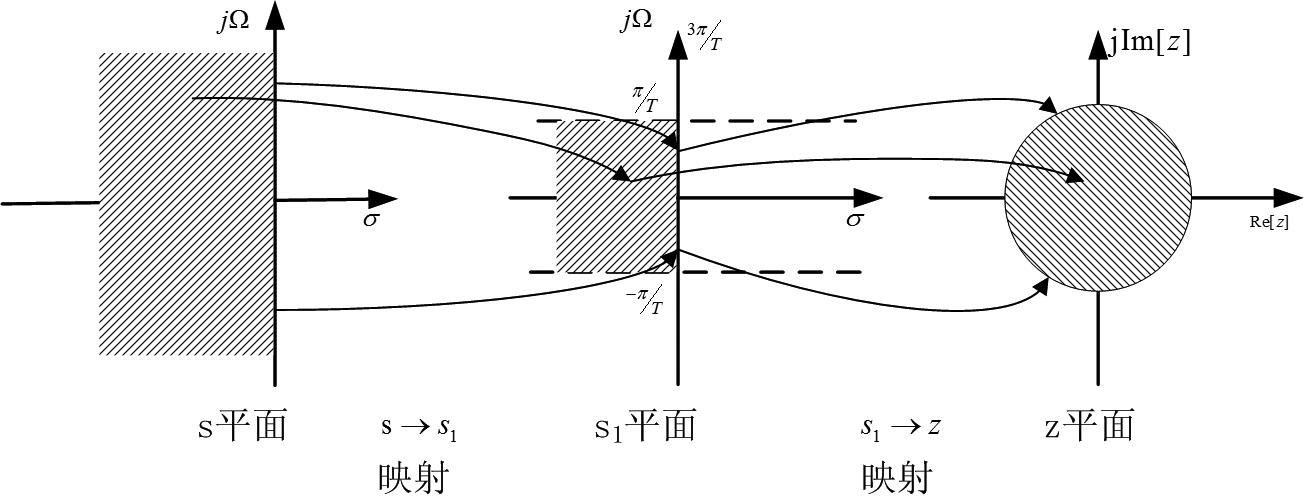
\includegraphics[width=0.80\textwidth]{fig18_BLT_yinsheguanxi.jpg}
%               \caption{s到s1到z平面的映射示意图}
%               %\vspace{-1.2cm}
%               %\label{}
%          \end{figure}
          \newpage
          $$\quad\quad
          \Omega = \frac{2}{T} \cdot tg(\frac{\Omega_1}{2}T)\quad\quad\quad\quad\quad\quad\quad\quad$$
          \textbf{讨论:}
          $$
          \left\{\begin{aligned}
            \;\Omega = 0 \quad      &\longrightarrow \Omega_1 = 0;\\
            \:\Omega = \infty\quad  &\longrightarrow \Omega_1 = \frac{\pi}{T};\\
            \Omega = -\infty &\longrightarrow \Omega_1 = -\frac{\pi}{T}.\\
          \end{aligned} \right.
          $$
          即,
          $$
          \left\{\begin{aligned}
            \mbox{ 当$\Omega$从$(0\rightarrow\infty)$变化时,}\\
            \mbox{$\Omega_1$从$(0\rightarrow \frac{\pi}{T})$变化。 \quad}\\
          \end{aligned} \right.
          $$
          %当$\Omega$从$(0\rightarrow\infty)$变化时,
          %$\Omega_1$从$(0\rightarrow)\frac{\pi}{T})$变化。
          注意,这些变换与$\sigma$无关,S平面的横坐标可取任意值。也就说可以看做是水平横带。
          $$\mbox{s平面}\quad  \rightarrow  \quad \mbox{水平横带区域(宽$\frac{2\pi}{T}$)}$$
      \newpage
      \item [2] $s_1 \longrightarrow z\quad\quad$  (单值的,脉冲响应不变)
          \begin{figure}[h]
               \centering
               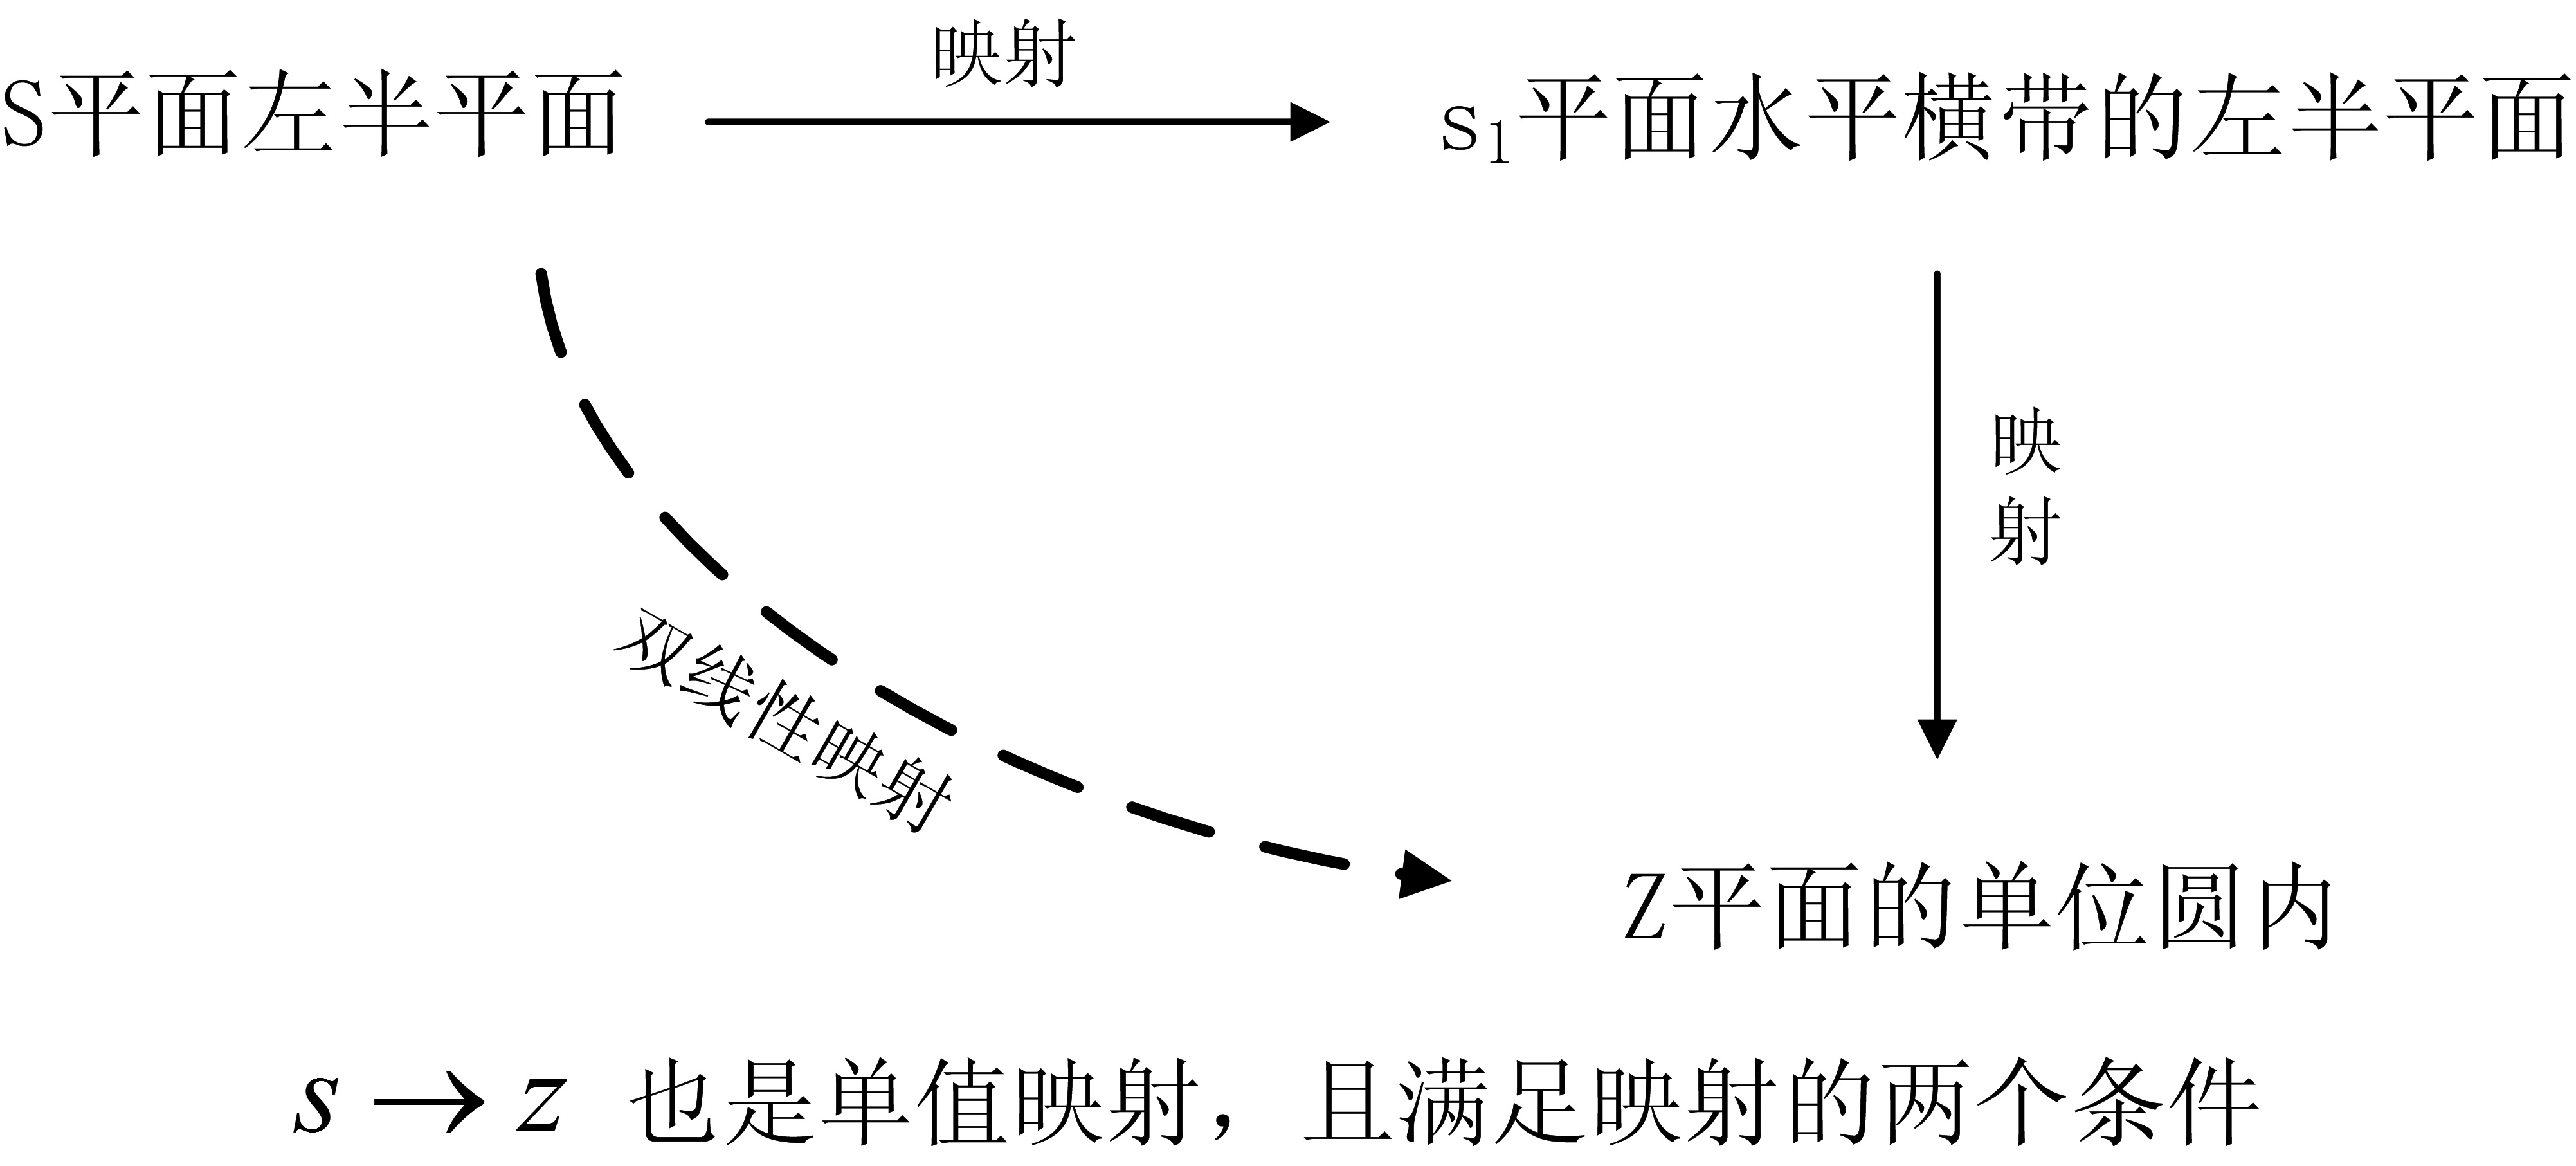
\includegraphics[width=0.5\textwidth]{fig19_BLT_shiyitu.jpg}
               %\caption{s到s1到z平面的映射示意图}
               %\label{}
          \end{figure}
          %$$s\longrightarrow z\quad\quad\mbox{也是单值映射,且满足映射的两个条件}$$
          \begin{center}
          s到s1到z平面的映射示意图
          \end{center}
          \begin{figure}[h]
               \centering
               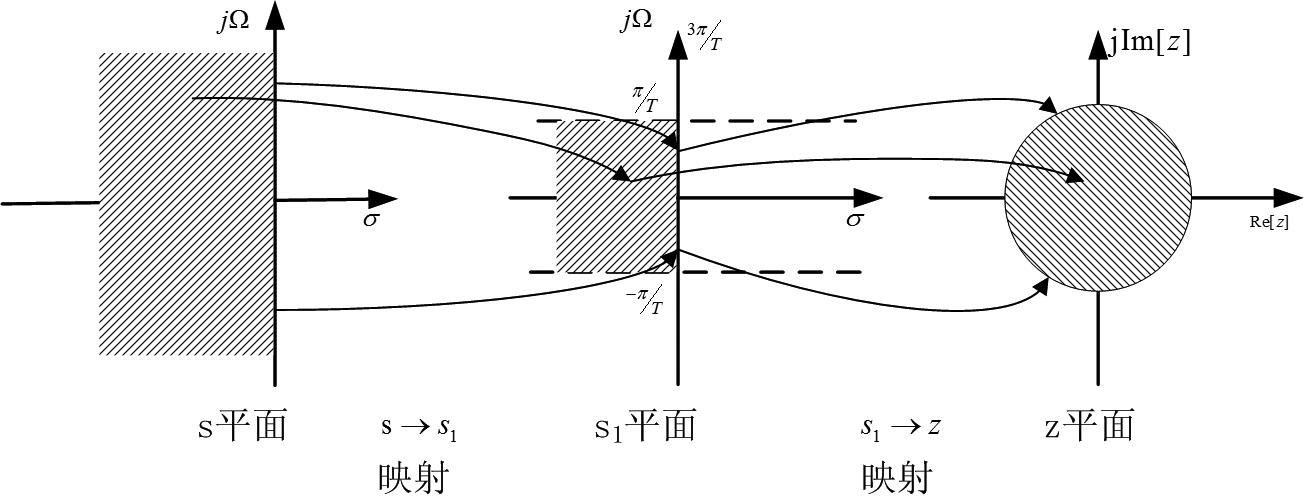
\includegraphics[width=0.650\textwidth]{fig18_BLT_yinsheguanxi.jpg}
               %\caption{s到s1到z平面的映射示意图}
               %\vspace{-1.2cm}
               %\label{}
          \end{figure}
          \begin{center}
          s到s1到z平面的映射示意图
          \end{center}
      \newpage
      \item  $\omega \longrightarrow \Omega$的关系
          $$
          \left\{\begin{aligned}
            \Omega &= \frac{2}{T} \cdot tg(\frac{\Omega_1}{2}T)\\
            \omega &= \Omega_1 T\quad\mbox{(脉冲响应不变法)}\\
          \end{aligned} \right.
          $$
          可得:
          %\begin{dablock}
          $$\Omega = \frac{2}{T} \cdot tg(\frac{\omega}{2})$$
          %\end{dablock}
          \textbf{说明}
          \begin{enumerate}
            \item $\omega = \Omega_1 T$是脉冲响应不变法得到的映射。
            \item 且有:
          $$
          \left\{\begin{aligned}
            \Omega:(0\rightarrow\infty) &\Rightarrow \Omega_1:(0\rightarrow\frac{\pi}{T})\Rightarrow \omega:(0\rightarrow\pi)\\
            \Omega:(-\infty\rightarrow 0)&\Rightarrow \Omega_1:(-\frac{\pi}{T}\rightarrow 0)\Rightarrow
            \omega:(-\pi \rightarrow 0)\\
          \end{aligned} \right.
          $$
          \end{enumerate}
          \newpage

          \begin{dablock}
          $$\Omega = \frac{2}{T} \cdot tg(\frac{\omega}{2})$$
          \end{dablock}
          \begin{figure}[h]
               \centering
               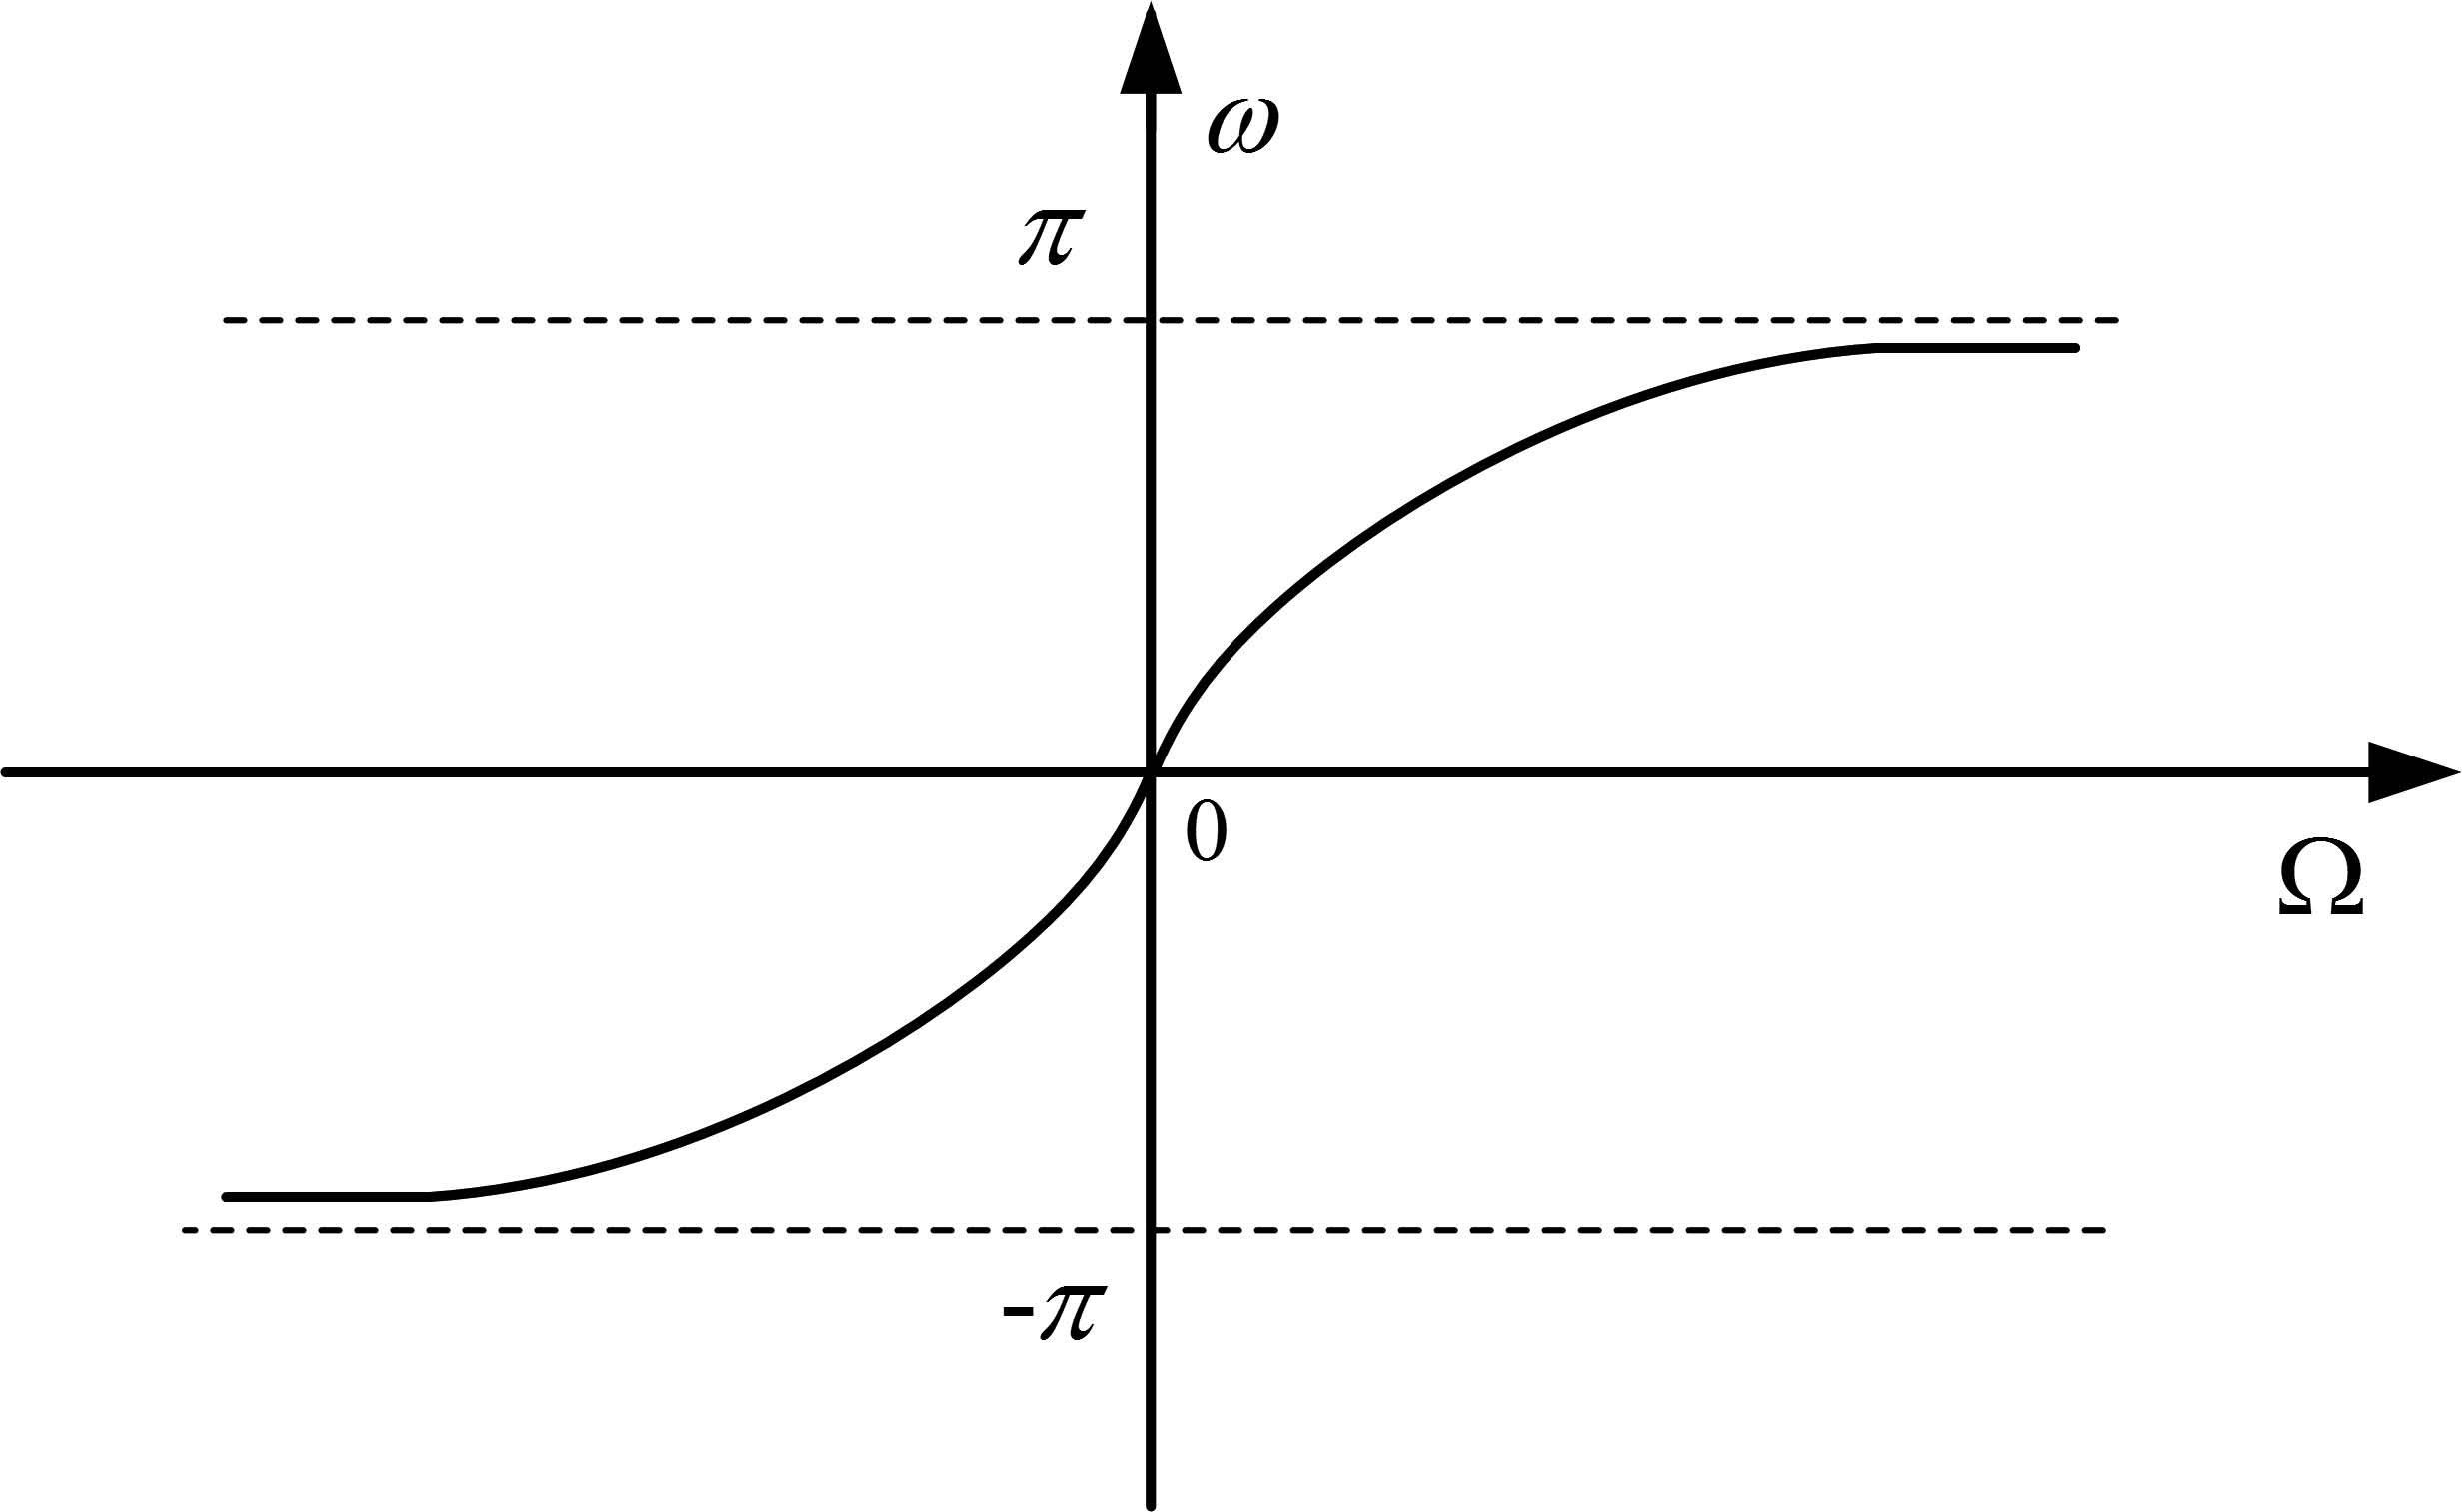
\includegraphics[width=0.6\textwidth]{fig20_BLT_pinlvguanxi.jpg}
               \caption{双线性变换频率映射关系示意图}
               %\label{}
          \end{figure}

    \end{enumerate}

\end{frame}
%%%%%%%%%%%%%%%%%%%%%%%%%%%%%%%%%%%%%%%%%%%%%%%%%%%%%%%%%%%%%%%%%%%%%%%%%%%%%%%%%%%%%%%%%%%%%%%


%%%%%%%%%%%%%%%%%%%%%%%%%%%%%%%%%%%%%%%%%%%%%%%%%%%%%%%%%%%%%%%%%%%%%%%%%%%%%%%%%%%%%%%%%%%%%%
\begin{frame}[shrink]\frametitle{}%[allowframebreaks][shrink]
\textbf{三、BLT的特点}
    \begin{enumerate}
      \item 优点:无频率混叠。
      \item 缺点:映射前后频率为非线性关系,直接影响到所涉及DF的频率响应
          能否逼真的模仿AF的频率响应。
    \end{enumerate}
    \textbf{解释:}
    \begin{enumerate}
      \item
          BLT方法将$\Omega$轴($0,\infty)$,压缩到$\omega$轴$(0,\pi)$,且为一一映射,
          但为非均匀压缩。
          \begin{figure}[h]
               \centering
               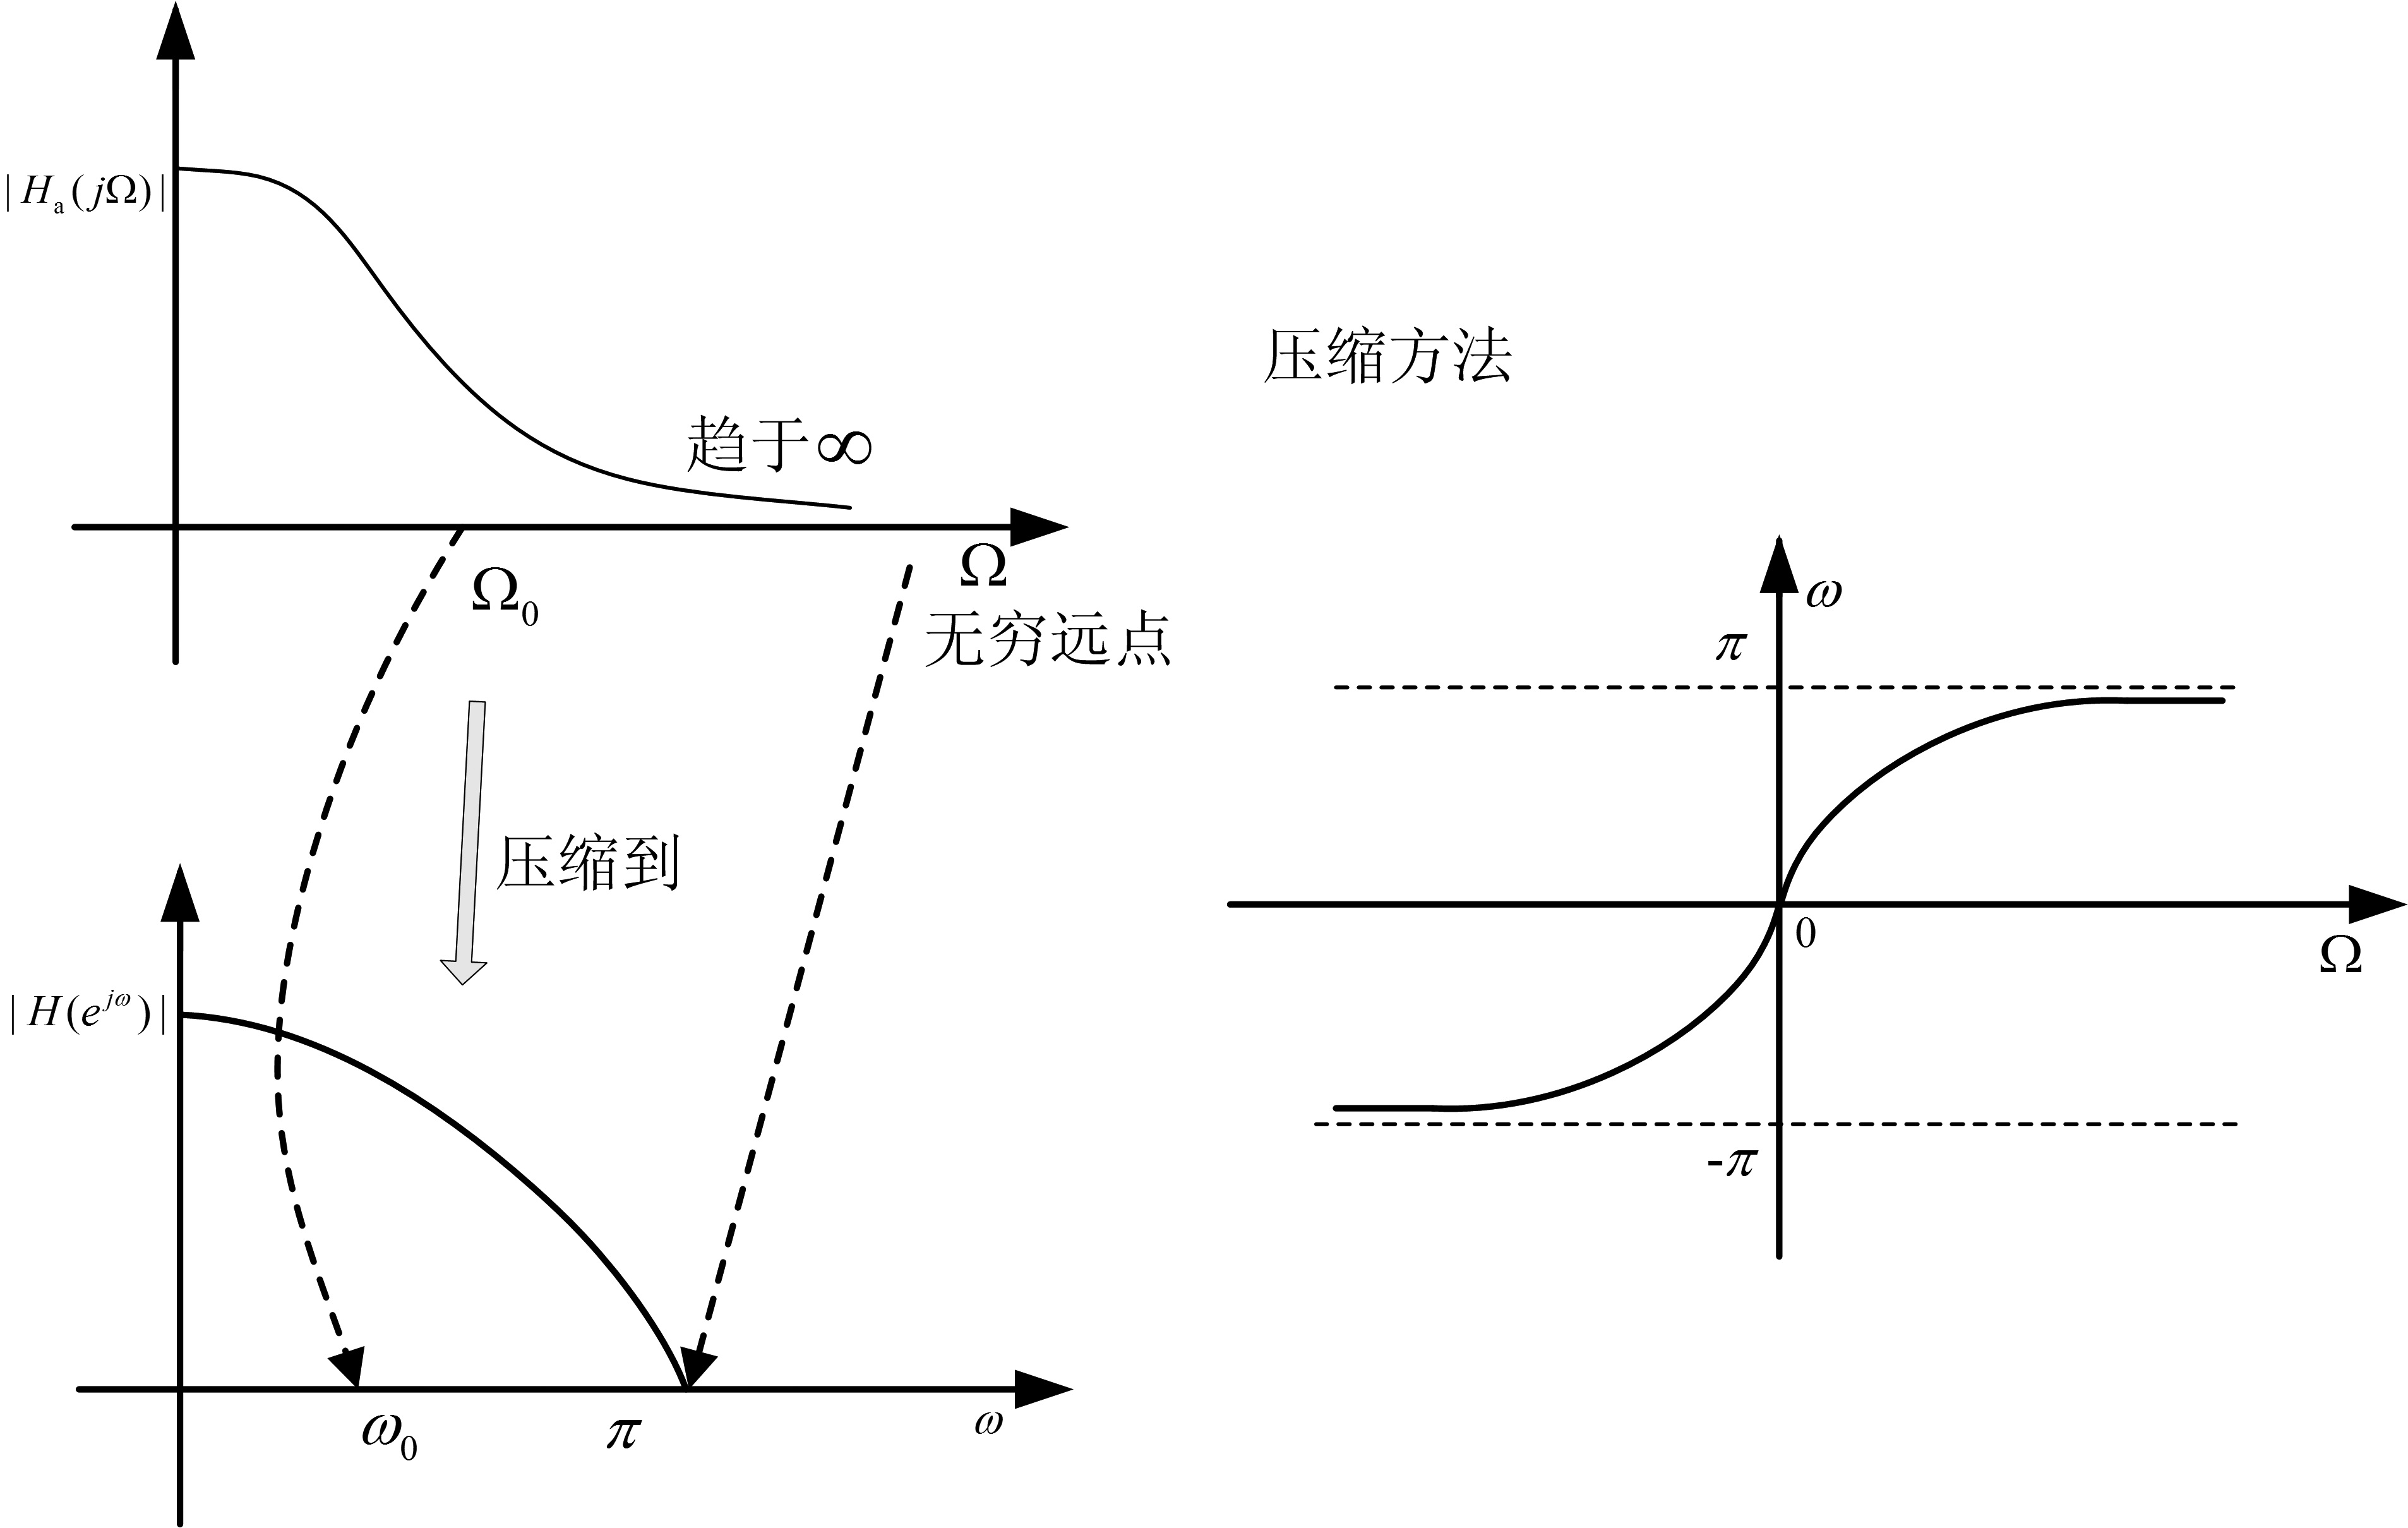
\includegraphics[width=0.6\textwidth]{fig21_BLT_feijunyunyasuo.jpg}
               %\caption{非均匀压缩变换示意图}
               %\label{}
          \end{figure}
      \item 适用范围:适用于具有片段常数特性的滤波器,可设计高通、低通、带通、带阻滤波器。
    \end{enumerate}
\end{frame}
%%%%%%%%%%%%%%%%%%%%%%%%%%%%%%%%%%%%%%%%%%%%%%%%%%%%%%%%%%%%%%%%%%%%%%%%%%%%%%%%%%%%%%%%%%%%%%%

\subsection{6.4.2 LP-DF完整设计方法}
%%%%%%%%%%%%%%%%%%%%%%%%%%%%%%%%%%%%%%%%%%%%%%%%%%%%%%%%%%%%%%%%%%%%%%%%%%%%%%%%%%%%%%%%%%%%%%
\begin{frame}[shrink]\frametitle{LP-DF完整设计方法}%[allowframebreaks][shrink]
假设给定技术参数:$(\omega_p,\alpha_p),(\omega_s,\alpha_s)$,
\begin{enumerate}
  \item
      将设计的LP-DF参数转变为相应的LP-AF的技术指标
      $(\Omega_p,\alpha_p),(\Omega_s,\alpha_s)$,
  \item
      设计LP-AF,得到$H_a(s)$
      $$
      \left\{ \begin{aligned}
        1) &\quad \mbox{求N,$\Omega_c\rightarrow|H_a(j\Omega|^2$}\\
        2) &\quad \mbox{查表,得到$H_a(p)$}\\
        3) &\quad \mbox{去归一化,$H_a(s)= H_a(p)|_{p=\frac{s}{\Omega_c}}$}\\
      \end{aligned} \right.
      $$
  \item
      $H_a(s)\underrightarrow{\quad\mbox{映射}\quad}H(z)$
      \begin{itemize}
        \item 脉冲响应不变法
        \item 双线性变换法
      \end{itemize}
\end{enumerate}
\end{frame}
%%%%%%%%%%%%%%%%%%%%%%%%%%%%%%%%%%%%%%%%%%%%%%%%%%%%%%%%%%%%%%%%%%%%%%%%%%%%%%%%%%%%%%%%%%%%%%%

\subsection{6.4.3 其他需要注意的问题}
%%%%%%%%%%%%%%%%%%%%%%%%%%%%%%%%%%%%%%%%%%%%%%%%%%%%%%%%%%%%%%%%%%%%%%%%%%%%%%%%%%%%%%%%%%%%%%
\begin{frame}[shrink]\frametitle{一、技术指标参数的转换}%[allowframebreaks][shrink]

%\textbf{一、技术指标参数的转换}
\begin{enumerate}
  \item [1] 说明:

      \begin{enumerate}
        \item [(a)] LP-DF指标可用三种形式给出。
              $$(\omega_p,\alpha_p)\quad\quad(\Omega_p,\alpha_p)
              \quad\quad(f_p,\alpha_p)$$
        \item [(b)] 数字域频率$\omega$及其对应的模拟域频率的关系总是不变的。
              $$\omega = \Omega T = 2\pi f T = \frac{2\pi f}{f_s}$$
        \par \textbf{注:}数字域频率是模拟角频率对采样频率的归一化频率。\par
              单位分别为:
              $$
              \left\{ \begin{aligned}
                f      &\quad  :\quad Hz\quad\quad\quad\quad\quad\quad\quad\quad
                \quad\quad\quad\quad\quad\quad\quad\quad\quad\quad\quad\quad\\
                \Omega &\quad :\quad rad/s \\
                \omega &\quad :\quad rad\\
              \end{aligned} \right.
              $$
              \end{enumerate}

  \item [2] 将设计的LP-DF技术指标转换为相应的LP-AF的技术指标时,转换的方式将由采用的\textbf{映射方式}决定:

\end{enumerate}
\end{frame}
%%%%%%%%%%%%%%%%%%%%%%%%%%%%%%%%%%%%%%%%%%%%%%%%%%%%%%%%%%%%%%%%%%%%%%%%%%%%%%%%%%%%%%%%%%%%%%%


%%%%%%%%%%%%%%%%%%%%%%%%%%%%%%%%%%%%%%%%%%%%%%%%%%%%%%%%%%%%%%%%%%%%%%%%%%%%%%%%%%%%%%%%%%%%%%
\begin{frame}[shrink]\frametitle{}%[allowframebreaks][shrink]
%二、映射前后$\Omega\rightarrow\omega$的关系

%    将设计的LP-DF技术指标转换为相应的LP-AF的技术指标时,转换的方式将由采用的\textbf{映射方式}决定:
%    $$
%      \left\{ \begin{aligned}
%        \mbox{脉冲法}     &\quad  :\quad \omega = \Omega \cdot T
%                            \quad\quad\quad\quad\quad\quad\quad\quad
%        \quad\quad\quad\quad\quad\quad\quad\quad\quad\quad\quad\quad\\
%        \mbox{BLT法}  &\quad :\quad \Omega = \frac{2}{T}tg(\frac{\omega}{2})\\
%      \end{aligned} \right.
%    $$
在转换滤波器技术指标时,
\begin{enumerate}
  \item 将给定的技术指标(三种方式之一)转换为数字域频率$\omega$形式,转换关系为:
     $$\omega = \Omega T = 2\pi f T = \frac{2\pi f}{f_s}$$
  \item 在数字滤波器技术指标转换为模拟滤波器技术指标时,频率映射方式遵循后期系统函数的映射方式:
      $$
      \left\{ \begin{aligned}
        \mbox{脉冲法}     &\quad  :\quad \omega = \Omega \cdot T
                            \quad\quad\quad\quad\quad\quad\quad\quad
        \quad\quad\quad\quad\quad\quad\quad\quad\quad\quad\quad\quad\\
        \mbox{BLT法}  &\quad :\quad \Omega = \frac{2}{T}tg(\frac{\omega}{2})\\
      \end{aligned} \right.
    $$

\end{enumerate}
\end{frame}
%%%%%%%%%%%%%%%%%%%%%%%%%%%%%%%%%%%%%%%%%%%%%%%%%%%%%%%%%%%%%%%%%%%%%%%%%%%%%%%%%%%%%%%%%%%%%%%


%%%%%%%%%%%%%%%%%%%%%%%%%%%%%%%%%%%%%%%%%%%%%%%%%%%%%%%%%%%%%%%%%%%%%%%%%%%%%%%%%%%%%%%%%%%%%%
\begin{frame}[shrink]\frametitle{}%[allowframebreaks][shrink]
\begin{example} 以两种不同的映射方法,将数字滤波器技术指标$\omega_p$$=0.4\pi\ rad$,$\alpha_p$$ = 3dB$转换为模拟滤波器技术指标,设$T = \frac{1}{2000}s$
\par   解:
   \begin{enumerate}
     \item 脉冲法:  $\quad\quad \omega = \Omega \cdot T $
     $$\therefore\quad \Omega_p = \frac{\omega_p}{T} =
       \frac{0.4\pi}{1/2000} = 800\pi\quad rad/s \quad$$
     $$  \mbox{或:} f_p = \frac{\Omega_p}{2\pi}= 400Hz$$
     \item BLT法:$\quad\quad\Omega = \frac{2}{T}tg(\frac{\omega}{2}) $  \quad (预畸变)
     $$\therefore\quad \Omega_p = \frac{2}{T}tg(\frac{\omega_p}{2})
       =4000tg(0.2\pi) = 2906\quad rad/s \quad$$
     $$  \mbox{或:} f_p = \frac{\Omega_p}{2\pi}= 463Hz$$

   \end{enumerate}

\end{example}
\end{frame}
%%%%%%%%%%%%%%%%%%%%%%%%%%%%%%%%%%%%%%%%%%%%%%%%%%%%%%%%%%%%%%%%%%%%%%%%%%%%%%%%%%%%%%%%%%%%%%%


%%%%%%%%%%%%%%%%%%%%%%%%%%%%%%%%%%%%%%%%%%%%%%%%%%%%%%%%%%%%%%%%%%%%%%%%%%%%%%%%%%%%%%%%%%%%%%
\begin{frame}[shrink]\frametitle{}%[allowframebreaks][shrink]
\textbf{三、预畸变的解释}%(双线性变换法所特有)

\begin{figure}[h]
\centering
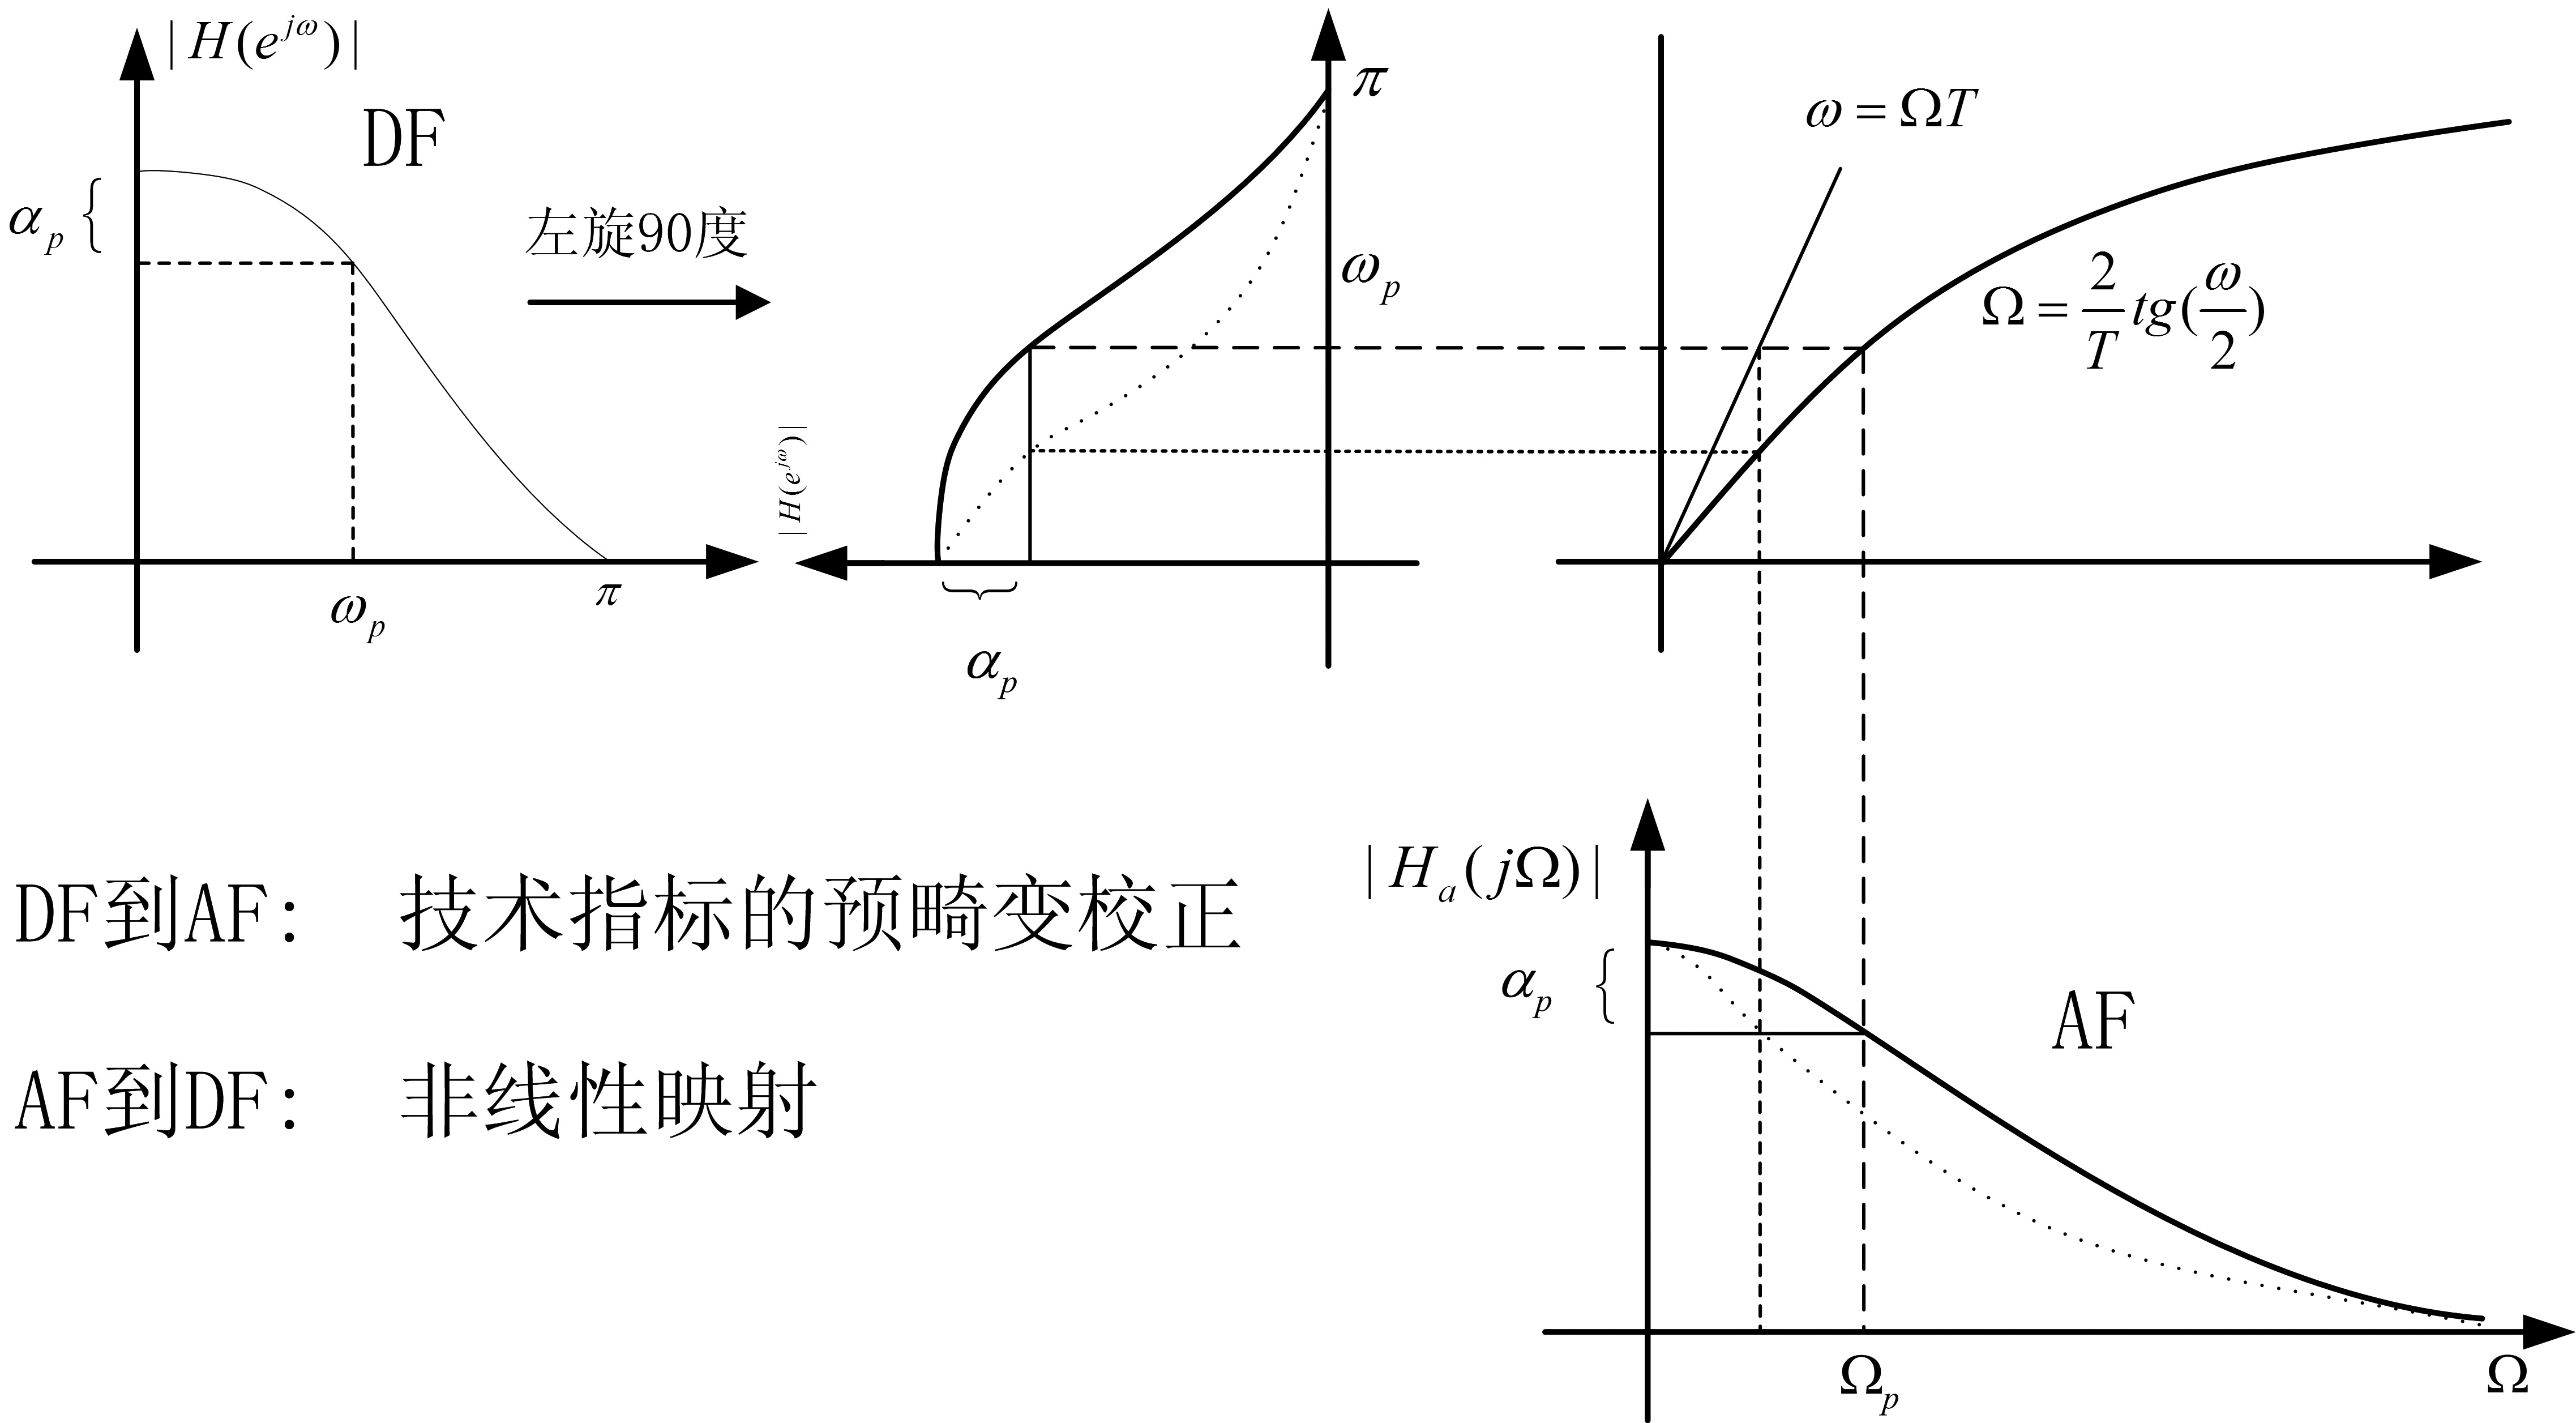
\includegraphics[width=0.9\textwidth]{fig22_BLT_yujibian.jpg}
%\caption{非均匀压缩变换示意图}
\label{}
\end{figure}
\end{frame}
%%%%%%%%%%%%%%%%%%%%%%%%%%%%%%%%%%%%%%%%%%%%%%%%%%%%%%%%%%%%%%%%%%%%%%%%%%%%%%%%%%%%%%%%%%%%%%%
\section*{例题}
%
\subsection*{例题1}
%%%%%%%%%%%%%%%%%%%%%%%%%%%%%%%%%%%%%%%%%%%%%%%%%%%%%%%%%%%%%%%%%%%%%%%%%%%%%%%%%%%%%%%%%%%%%%
\begin{frame}\frametitle{}%[allowframebreaks][shrink]
\begin{example}
请设计一个低通IIR-DF,要求:
\begin{enumerate}
  \item[(1)] 模拟滤波器采用Butterworth型,映射方法选用双线性变换法;
  \item[(2)] 当$0\leqslant f \leqslant 25Hz$时,衰减$\leqslant 3\quad dB$;
  \item[(3)] 当$0\leqslant f \leqslant 50Hz$时,衰减$\geqslant 38\quad dB$;
  \item[(4)] 取样频率: $f_0 = 200Hz$
\end{enumerate}
\end{example}
\textbf{解:}
  首先,解题步骤:

  \begin{enumerate}
     \item 将LP-DF技术要求,转化为LP-AF技术要求。
     \item 设计LP-AF;
         \begin{enumerate}
           \item 由技术指标求N、$\Omega_c$;
           \item 查表得$H_a(p)$;
           \item 去归一化,得到$H_a(s)$。
         \end{enumerate}
     \item $H_a(s)\longrightarrow H(z)$
   \end{enumerate}

\end{frame}
%%%%%%%%%%%%%%%%%%%%%%%%%%%%%%%%%%%%%%%%%%%%%%%%%%%%%%%%%%%%%%%%%%%%%%%%%%%%%%%%%%%%%%%%%%%%%%%


%%%%%%%%%%%%%%%%%%%%%%%%%%%%%%%%%%%%%%%%%%%%%%%%%%%%%%%%%%%%%%%%%%%%%%%%%%%%%%%%%%%%%%%%%%%%%%
\begin{frame}[allowframebreaks]\frametitle{}%[allowframebreaks][shrink]
\quad\newline\quad
$1^0\quad$ 技术指标的转换:
\quad\newline\quad
  \par 由题意知,这里DF技术指标由$f_p,f_s$的形式给出,需转换为$\omega_p,\omega_s$的形式。
  $$
  \left\{ \begin{aligned}
      f_p      &= 25Hz\quad\Longrightarrow
                  \omega_p = 2\pi \frac{f_p}{f_0} = 0.25\pi\quad rad\\
      \alpha_p &= 3 dB  \\
      \end{aligned} \right.
  $$
  $$
  \left\{ \begin{aligned}
      f_s      &= 50Hz\quad\Longrightarrow
                  \omega_s = 2\pi \frac{f_s}{f_0} = 0.5\pi\quad rad\\
      \alpha_s &= 38 dB  \\
      \end{aligned} \right.
  $$
  \newpage
  \quad\newline\quad
  下一步,将DF技术指标转换为AF技术指标,需根据所选的映射方法规定的映射关系转换。

  $$\mbox{对于BLT法:}\quad\quad\quad\quad\quad\quad
  \Omega = \frac{2}{T}tg(\frac{\omega}{2})$$
  则有:
  $$
  \left\{ \begin{aligned}
      \Omega_p      &= \frac{2}{T}tg(\frac{\omega_p}{2})
                     = 2f_0 \cdot tg(\frac{\omega_p}{2})= 400tg(\frac{\pi}{8})
                     = 165.685\quad rad/s\\
      \alpha_p &= 3 dB  \\
      \end{aligned} \right.
  $$
  $$
  \left\{ \begin{aligned}
      \Omega_s      &= \frac{2}{T}tg(\frac{\omega_s}{2})
                     = 2f_0 \cdot tg(\frac{\omega_s}{2})= 400tg(\frac{\pi}{4})
                     = 400\quad rad/s\quad\quad\\
      \alpha_s &= 38 dB  \\
      \end{aligned} \right.
  $$
  \newpage
  $2^0\quad$  设计LP-AF
  \begin{enumerate}
    \item [(1)]确定阶数N,$\Omega_c$;
        $$\left(\frac{\Omega_p}{\Omega_s}\right)^{2N}
           = \frac{10^{\frac{\alpha_p}{10}}-1}{10^{\frac{\alpha_s}{10}}-1}$$
        代入上述参数,可得:
        $$\left(\frac{165.685}{400}\right)^{2N}
           = \frac{10^{0.3}-1}{10^{3.8}-1}$$
        得:$N =4.96$,因为N需为整数,取N=5.
        $$\alpha_{p} = 3dB\Longrightarrow \Omega_c = \Omega_p = 165.685\quad rad/s$$
    \newpage
    \item [(2)]根据,N=5,查表可得:
        $$H_a(p) = \frac{1}{(p^2 + 0.618p+1)(p^2 + 1.618p+1)(p+1)}$$
    \item [(3)]去归一化;
%        $$H_a(s) = H_a(p)|_{p=\frac{s}{\Omega}}
%          = \frac{\Omega_c^5}{(s^2 + 0.618s\Omega+\Omega_c^2)(s^2 + 1.618s\Omega+\Omega_c^2)(s+\Omega_c)}$$
    \begin{equation*}
      \begin{split}
         H_a(s) &= H_a(p)\Big|_{p=\frac{s\;}{\Omega_c}} \\
                &= \frac{\Omega_c^5}{(s^2 + 0.618s\cdot\Omega_c+\Omega_c^2)(s^2 + 1.618s\cdot\Omega_c+\Omega_c^2)(s+\Omega_c)}
       \end{split}
    \end{equation*}
        其实不必计算出来,后面还可以化简。
  \end{enumerate}
  \newpage
  $3^0\quad$  $H_a(s)\longrightarrow H(z)$
  $$H(z) = H_a(s)\Big|_{s=\frac{2}{T}\frac{1-z^{-1}}{1+z^{-1}}}\quad\quad\quad\quad
  H_a(s) = H_a(p)\Big|_{p=\frac{s}{\Omega_c}}$$
  $$\Longrightarrow\quad\quad H(z) = \left[H_a(p)|_{p=\frac{s}{\Omega_c}}\right]
  _{s=\frac{2}{T}\frac{1-z^{-1}}{1+z^{-1}}}
  = H_a(p)\Big|_{p=\frac{2}{\Omega_c T}\frac{1-z^{-1}}{1+z^{-1}}}$$
  $$\mbox{而:}\quad\quad\quad
  \Omega_c = \frac{2}{T}tg(\frac{\omega_c}{2}) \Longrightarrow
  \frac{2}{\Omega_c T} = ctg(\frac{\omega_c}{2})$$
  \begin{dablock}
  $$\therefore\quad\quad
  H(z) = H_a(p)\Big|_{p=ctg(\frac{\omega_c}{2})\frac{1-z^{-1}}{1+z^{-1}}}$$
  \end{dablock}
  本题中:
  $$\omega_c = \frac{\pi}{4}\Longrightarrow p = 2.414\frac{1-z^{-1}}{1+z^{-1}}$$
  $$\therefore\quad\quad\quad\quad\quad
  H(z) = H_a(p)\Big|_{p=2.414\frac{1-z^{-1}}{1+z^{-1}}}$$
  \newpage
  \begin{equation*}
  \begin{split}
  H(z) &= H_a(p)\Big|_{p=2.414\frac{1-z^{-1}}{1+z^{-1}}}\\
       &=\frac{1}{((2.414\frac{1-z^{-1}}{1+z^{-1}})^2 + 0.618(2.414\frac{1-z^{-1}}{1+z^{-1}})+1)} \\
       &\quad\cdot \frac{1}{((2.414\frac{1-z^{-1}}{1+z^{-1}})^2 + 1.618(2.414\frac{1-z^{-1}}{1+z^{-1}})+1)}
       \cdot\frac{1}{(2.414\frac{1-z^{-1}}{1+z^{-1}}+1)}\\
       &=\frac{0.00382(1+2z^{-1}+z^{-2})}{1-1.16z^{-1}+0.642z^{-2}}
         \frac{1+2z^{-1}+z^{-2}}{1-0.9z^{-1}+0.273z^{-2}}
         \frac{1+z^{-1}}{1-0.414z^{-1}}\\
  \end{split}
  \end{equation*}

  $4^0\quad$ 画出其网络结构。
  \begin{figure}[h]
    \centering
    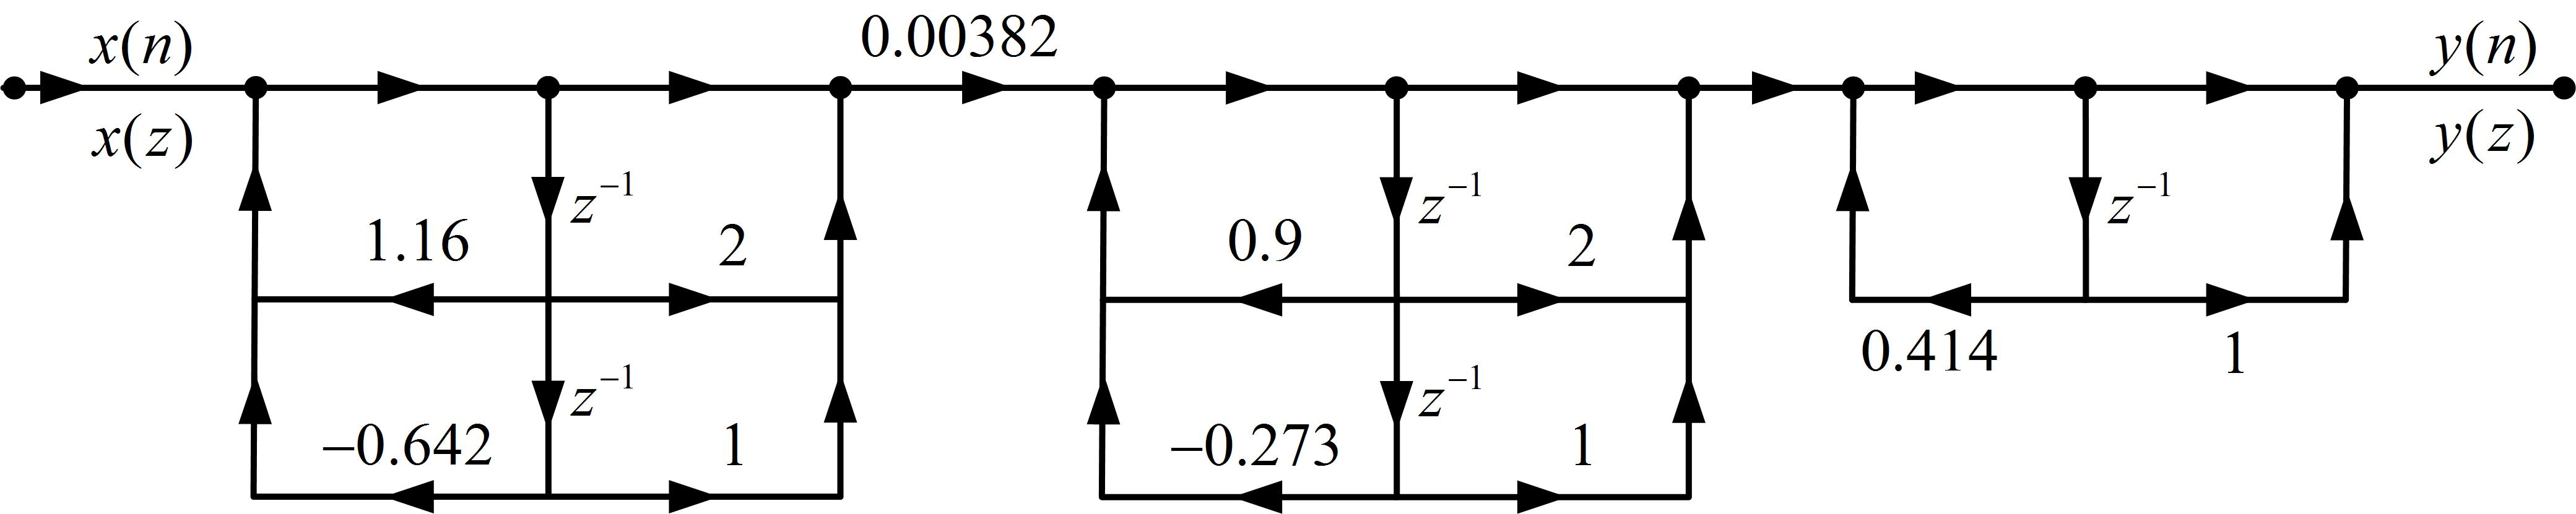
\includegraphics[width=0.9\textwidth]{fig23_example1.jpg}
    %\caption{非均匀压缩变换示意图}
    \label{}
  \end{figure}
\end{frame}
%%%%%%%%%%%%%%%%%%%%%%%%%%%%%%%%%%%%%%%%%%%%%%%%%%%%%%%%%%%%%%%%%%%%%%%%%%%%%%%%%%%%%%%%%%%%%%%

\subsection*{例题2}
%%%%%%%%%%%%%%%%%%%%%%%%%%%%%%%%%%%%%%%%%%%%%%%%%%%%%%%%%%%%%%%%%%%%%%%%%%%%%%%%%%%%%%%%%%%%%%
\begin{frame}[allowframebreaks]\frametitle{}%[allowframebreaks][shrink]
\begin{example}
用脉冲响应不变法设计一个3阶Butterworth滤波器(LP-DF),且$\omega_c = 1\quad rad$,
采样频率$f_0 = 2\pi\quad kHz$.
\end{example}
\par \textbf{解:}
\begin{enumerate}
  \item 求N,$\Omega_c$;
      依题意得:
      $$N=3,\qquad\qquad \Omega_c = \frac{\omega_c}{T}=\omega_c f_0 = 2\pi\times 10^3 \quad rad/s$$
  \item 查表得:
      $$N = 3\quad \Longrightarrow H_a(p) = \frac{1}{(p^2 + p+1)(p+1)}$$
      $$\mbox{去归一化:}\quad\quad\quad
      H_a(s) = H_a(p)\Big|_{p=\frac{s}{\Omega_c}}\quad\quad\mbox{代入可得$H_a(s)$}$$
      %也可以如下计算:
%      $$H_a(p) = \frac{1}{\prod_{k=0}^{N-1}(p-p_k)}\quad\quad
%      p_k = e^{j\pi\left[\frac{1}{2}+\frac{2k+1}{2N}\right]}$$
%      $$
%      \left\{ \begin{aligned}
%      k=0\quad\quad p_0&=e^{j\pi\frac{2}{3}}= -\frac{1}{2}+j\frac{\sqrt{3}}{2}\\
%      k=1\quad\quad p_1&=e^{j\pi[\frac{1}{2}+\frac{3}{6}]}= e^{j\pi}= -1\\
%      k=2\quad\quad p_2&=e^{j\pi[\frac{1}{2}+\frac{5}{6}]}= -\frac{1}{2}-j\frac{\sqrt{3}}{2}\\
%      \end{aligned} \right.
%      $$
%      $$H_a(p) = \frac{1}{(p-(-\frac{1}{2}+j\frac{\sqrt{3}}{2}))
%          (p-(-\frac{1}{2}-j\frac{\sqrt{3}}{2}))(p+1)}
%          = \frac{1}{(p^2 + p+1)(p+1)}$$
  \item 因式分解
  \end{enumerate}
  $$\mbox{令:}\quad H_a(p) = \frac{1}{p+1}+\frac{ap+b}{p^2+p+1}\quad\quad
  \Longrightarrow a=-1\quad b=0$$
  \begin{equation*}
  \begin{split}
  H_a(p)
           &= \frac{1}{p+1}-\frac{p}{p^2+p+1}\\
           &= \frac{1}{p+1}+
              \frac{-\frac{1}{2}+j\frac{\sqrt{3}}{6}}
                        {p+\frac{1}{2}+j\frac{\sqrt{3}}{2}}-
              \frac{\frac{1}{2}+j\frac{\sqrt{3}}{6}}
                        {p+\frac{1}{2}-j\frac{\sqrt{3}}{2}}\\
  \end{split}
  \end{equation*}
  $$\mbox{去归一化:}\quad\quad\quad  H_a(s) = H_a(p)\Big|_{p=\frac{s}{\Omega_c}}$$
  $$H_a(s)= \left[\frac{1}{s+\Omega_c}+
            \frac{-\frac{1}{2}+j\frac{\sqrt{3}}{6}}
                {s+(\frac{1}{2}+j\frac{\sqrt{3}}{2})\Omega_c}-
            \frac{\frac{1}{2}+j\frac{\sqrt{3}}{6}}
                {s+(\frac{1}{2}-j\frac{\sqrt{3}}{2})\Omega_c}\right]\cdot\Omega_c
  $$
\end{frame}
%%%%%%%%%%%%%%%%%%%%%%%%%%%%%%%%%%%%%%%%%%%%%%%%%%%%%%%%%%%%%%%%%%%%%%%%%%%%%%%%%%%%%%%%%%%%%%%


%%%%%%%%%%%%%%%%%%%%%%%%%%%%%%%%%%%%%%%%%%%%%%%%%%%%%%%%%%%%%%%%%%%%%%%%%%%%%%%%%%%%%%%%%%%%%%
\begin{frame}[shrink]\frametitle{}%[allowframebreaks][shrink]
  $$H(z) = \sum_{i=1}^{M}\frac{A_i}{1-e^{s_i T}z^{-1}}\quad\quad\quad
  (\frac{A_i}{s-s_i}\longrightarrow \frac{A_i}{1-e^{s_i T}z^{-1}})\quad\quad\quad$$
  \begin{equation*}
  \begin{split}
  H(z) &= \left[
              \frac{1}{1-e^{-\Omega_c T}z^{-1}}+
              \frac{-\frac{1}{2}+j\frac{\sqrt{3}}{6}}
                  {1-e^{-(\frac{1}{2}+j\frac{\sqrt{3}}{2})\Omega_c T}z^{-1}}-
              \frac{\frac{1}{2}+j\frac{\sqrt{3}}{6}}
                  {1-e^{-(\frac{1}{2}-j\frac{\sqrt{3}}{2})\Omega_c T}z^{-1}}
              \right]\cdot\Omega_c\\
           &\quad   \mbox{而:}\quad\quad \Omega_c T = \omega_c = 1\\
           &= \left[\frac{-1-0.41z^{-1}}{1+1.1z^{-1} + 0.368z^{-2}}+
              \frac{1}{1-0.368z^{-1}}\right]\cdot\Omega_c\\
  \end{split}
  \end{equation*}
  \newline\newline\newline\newline\newline\newline\newline\newline
\end{frame}
%%%%%%%%%%%%%%%%%%%%%%%%%%%%%%%%%%%%%%%%%%%%%%%%%%%%%%%%%%%%%%%%%%%%%%%%%%%%%%%%%%%%%%%%%%%%%%%


%%%%%%%%%%%%%%%%%%%%%%%%%%%%%%%%%%%%%%%%%%%%%%%%%%%%%%%%%%%%%%%%%%%%%%%%%%%%%%%%%%%%%%%%%%%%%%
\begin{frame}[shrink]\frametitle{}%[allowframebreaks][shrink]
   \begin{enumerate}
  \item 画出网络结构图:
   \end{enumerate}
  \begin{figure}[h]
    \centering
    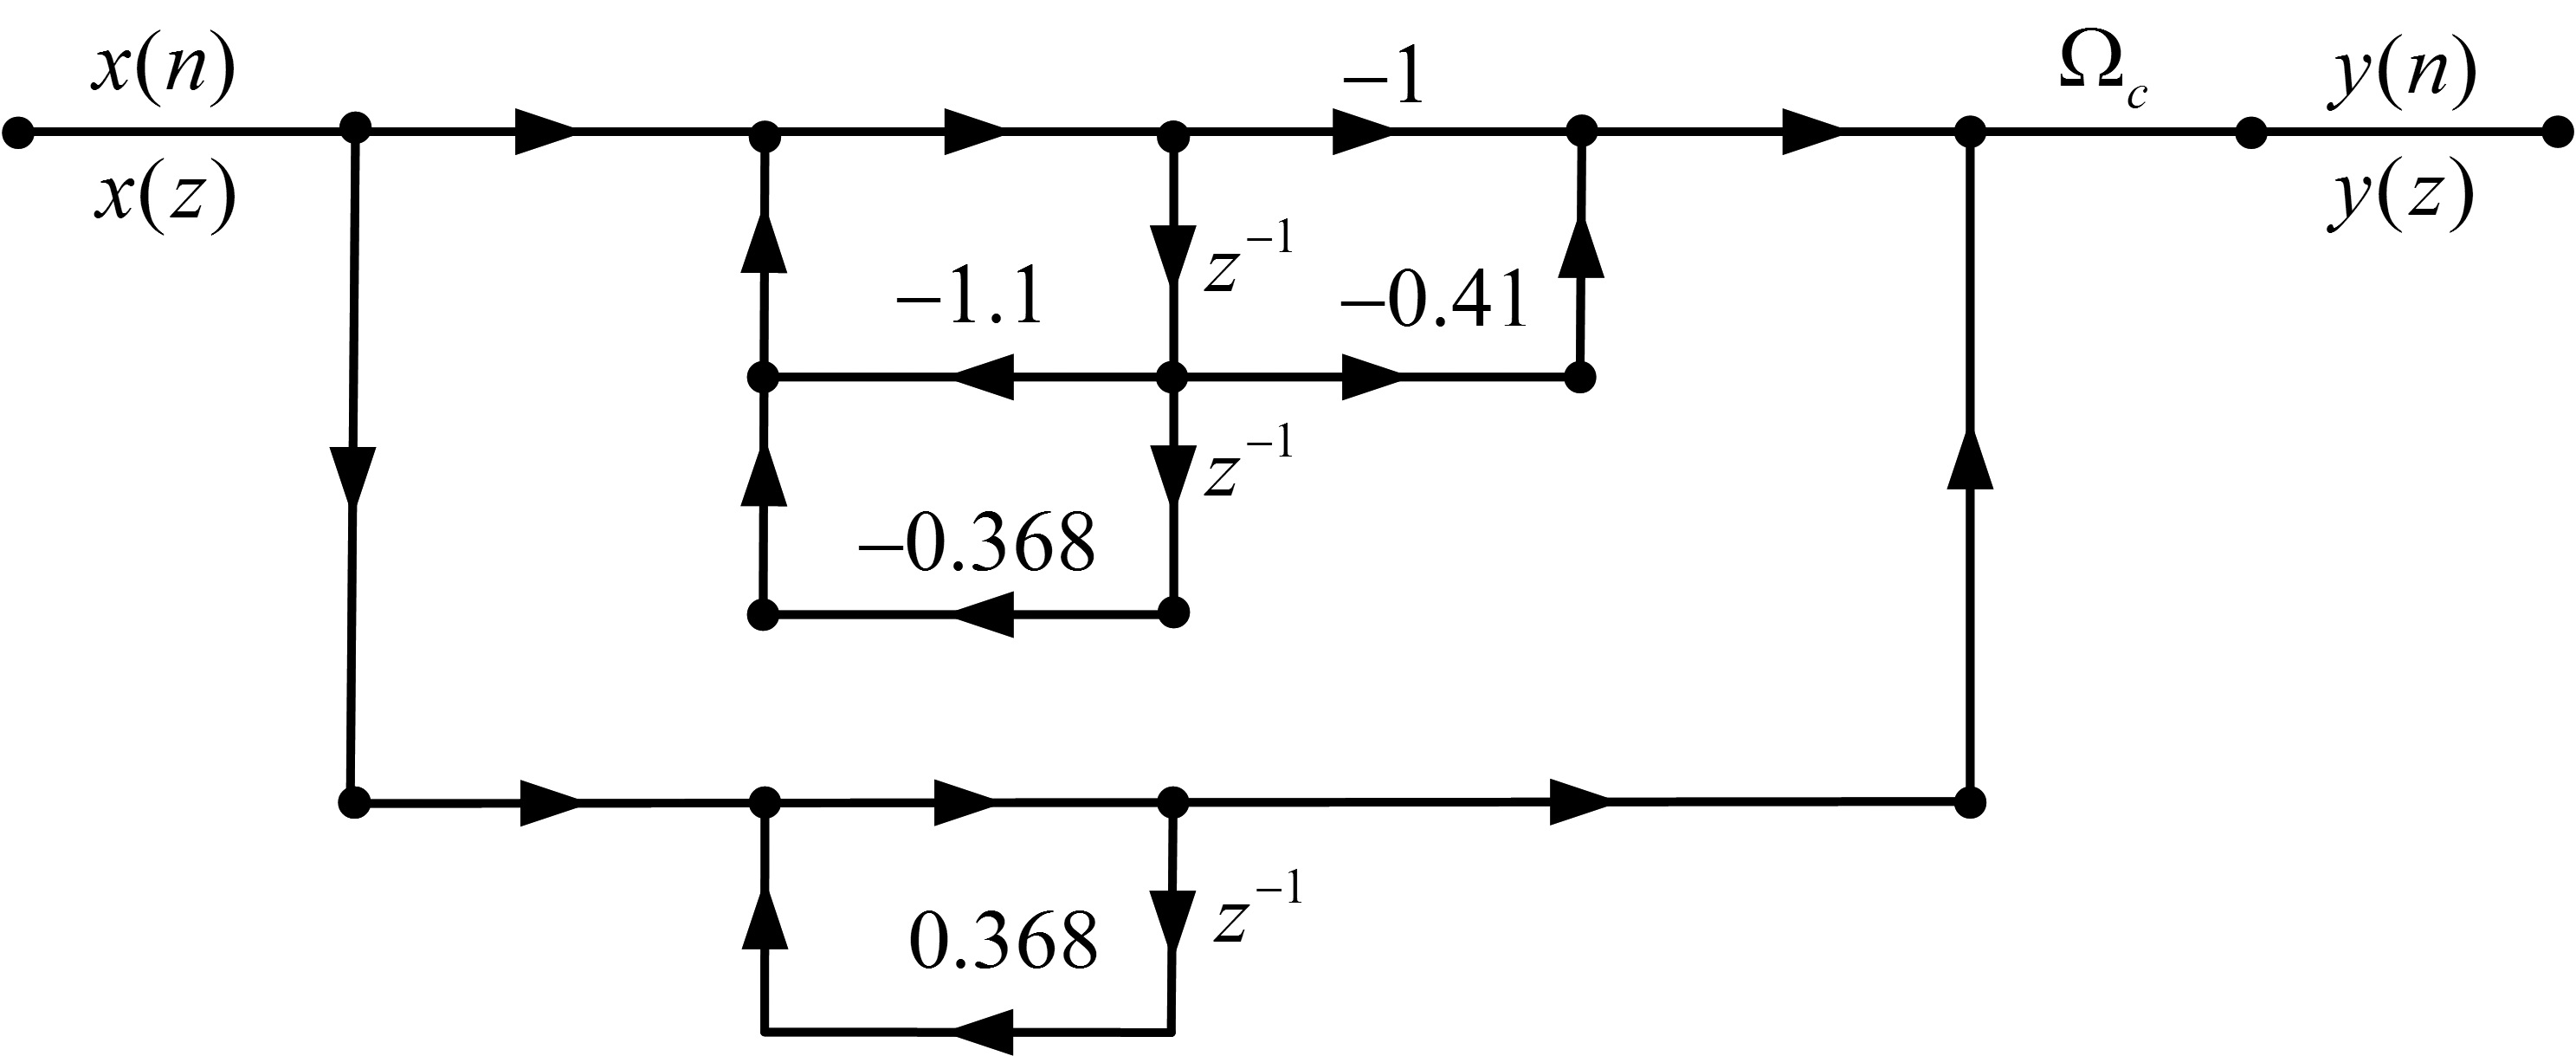
\includegraphics[width=0.85\textwidth]{fig24_example2.jpg}
    \caption{网络结构图}
    \label{}
  \end{figure}
\end{frame}
%%%%%%%%%%%%%%%%%%%%%%%%%%%%%%%%%%%%%%%%%%%%%%%%%%%%%%%%%%%%%%%%%%%%%%%%%%%%%%%%%%%%%%%%%%%%%%%

\subsection*{例题3}
%%%%%%%%%%%%%%%%%%%%%%%%%%%%%%%%%%%%%%%%%%%%%%%%%%%%%%%%%%%%%%%%%%%%%%%%%%%%%%%%%%%%%%%%%%%%%%
\begin{frame}[allowframebreaks]\frametitle{}%[allowframebreaks][shrink]
\begin{example}
用双线性变换法设计一个3阶Butterworth滤波器(LP-DF),采样频率$f_0 = 1.2kHz,\quad\omega_c = \frac{2}{3}\pi\quad rad$.
\end{example}
\textbf{解:}
$$\mbox{依题意有:}\quad\quad
N =3,\quad\quad \Omega_c = \frac{2}{T}tg(\frac{\omega_c}{2})=2.4\times\sqrt{3}\times 10^3$$
\par 查表得:
$$N = 3\quad \Longrightarrow H_a(p) = \frac{1}{(p^2 + p+1)(p+1)}$$
\newpage
$$\mbox{去归一化:}\quad\quad\quad
      H_a(s) = H_a(p)|_{p=\frac{s}{\Omega_c}}
\quad\quad\quad\quad\quad\quad\quad\quad\quad$$
$$\therefore\quad\quad H(z) = \left[H_a(p)\Big|_{p=\frac{s}{\Omega_c}}\right]
  _{s=\frac{2}{T}\frac{1-z^{-1}}{1+z^{-1}}}
  = H_a(p)\Big|_{p=ctg(\frac{\omega_c}{2})\frac{1-z^{-1}}{1+z^{-1}}}$$
%$$\therefore\quad\quad
%  \Omega_c = \frac{2}{T}tg(\frac{\omega_c}{2}) \Longrightarrow
%  \frac{2}{\Omega_c T} = ctg(\frac{\omega_c}{2})$$
\begin{equation*}
  \begin{split}
      \therefore\quad H(z)
           &= H_a(p)\Big|_{p=\frac{1}{\sqrt{3}}\frac{1-z^{-1}}{1+z^{-1}}}\\
           &= \frac{1}{\left[
              \frac{1}{3}(\frac{1-z^{-1}}{1+z^{-1}})^2 +
              \frac{1}{\sqrt{3}}\frac{1-z^{-1}}{1+z^{-1}}+1\right]
              (\frac{1}{\sqrt{3}}\frac{1-z^{-1}}{1+z^{-1}}+1)}\\
           &= \frac{9(1+z^{-1})^2}{(4+\sqrt{3})+4z^{-1}+(4-\sqrt{3})z^{-2}}\cdot
              \frac{1+z^{-1}}{3+\sqrt{3}+(3-\sqrt{3})z^{-1}}\\
           &= \frac{0.33(1+2z^{-1}+z^{-2})}{1+0.7z^{-1}+0.396z^{-2}}\cdot
              \frac{1+z^{-1}}{1+0.268z^{-1}}\\
  \end{split}
  \end{equation*}
  \newpage
  画出网络结构图:
  \begin{figure}[h]
    \centering
    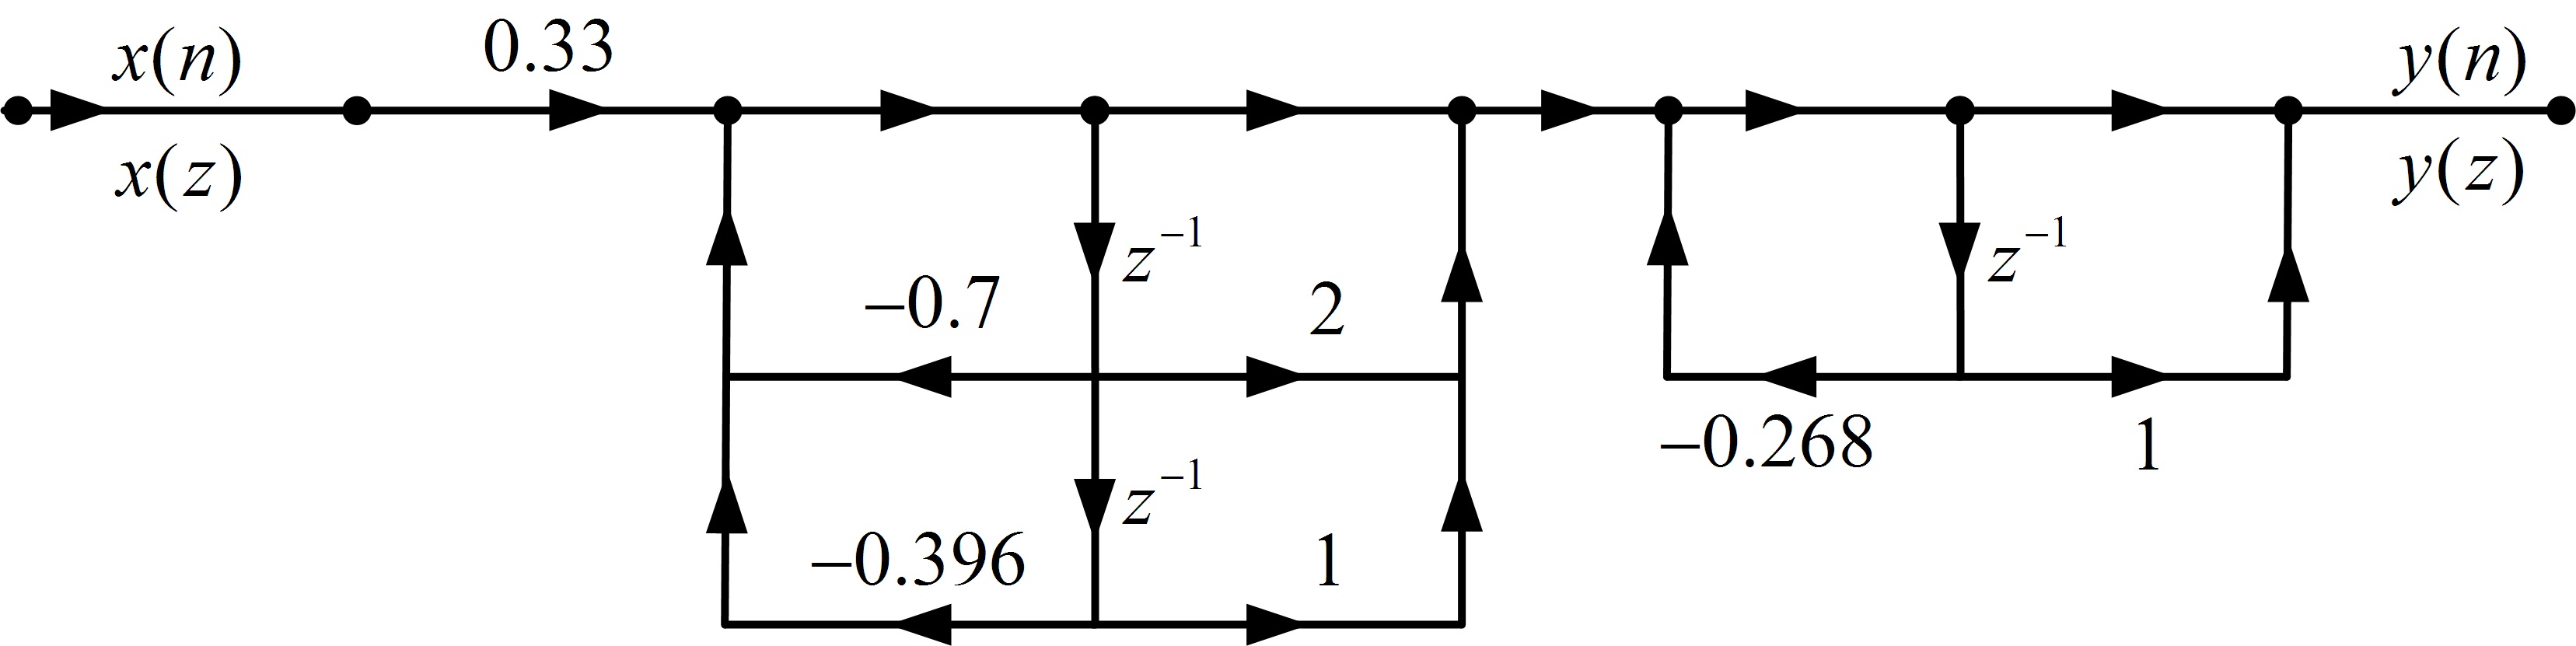
\includegraphics[width=0.85\textwidth]{fig25_example3.jpg}
    \caption{网络结构图}
    \label{}
  \end{figure}
\end{frame}
%%%%%%%%%%%%%%%%%%%%%%%%%%%%%%%%%%%%%%%%%%%%%%%%%%%%%%%%%%%%%%%%%%%%%%%%%%%%%%%%%%%%%%%%%%%%%%%


%%%%%%%%%%%%%%%%%%%%%%%%%%%%%%%%%%%%%%%%%%%%%%%%%%%%%%%%%%%%%%%%%%%%%%%%%%%%

\end{document}

